\documentclass[11pt,a4paper]{article}

\usepackage[utf8]{inputenc}
\usepackage[T1]{fontenc}
\usepackage{lmodern}
\usepackage{microtype}
\usepackage{xcolor}
\usepackage{geometry}
\usepackage{graphicx}
\usepackage{setspace}
\usepackage{fancyhdr}
\usepackage{caption}
\usepackage{booktabs}
\usepackage{amsmath}
\usepackage{amssymb}
\usepackage{tikz}
\usetikzlibrary{arrows.meta,positioning,calc,shapes.geometric}
\usepackage{longtable}
\IfFileExists{xurl.sty}{%
  \usepackage{xurl}%
}{%
  \PassOptionsToPackage{hyphens}{url}%
  \usepackage{url}%
}
\usepackage[hidelinks]{hyperref}
\usepackage{etoolbox}
\makeatletter
% Chaque \section numérotée commence sur une page (sauf la première du corps).
\pretocmd{\section}{\ifnum\c@section>\z@\clearpage\fi}{}{}
\makeatother

% Marges type mémoire / rapport d'ingénierie
\geometry{
  top=2.6cm,
  bottom=2.8cm,
  left=3cm,
  right=2.5cm,
  bindingoffset=0cm,
}
% Limite les débordements horizontaux (lignes fines, chemins \path, maths inline).
\setlength{\emergencystretch}{2.8em}
\tolerance=1600

% Liens et métadonnées PDF
\hypersetup{
  pdftitle={Quantum Bluff -- Final Project Report},
  pdfauthor={University of Strasbourg -- L3 Computer Science},
  pdfsubject={Capstone software engineering report},
  pdfkeywords={multiplayer games, Texas Hold'em, WebSocket, TypeScript, React, Node.js, Prisma, Redis, security},
  linktoc=all,
  bookmarksopen=true,
}
\setcounter{tocdepth}{2}

% Interligne confortable (corps du texte)
\onehalfspacing

% Couleur pour filets (page de garde)
\definecolor{HeadingRule}{RGB}{0,51,102}

% Légendes de figures / tableaux
\captionsetup{
  font=small,
  labelfont={bf,sf},
  textfont=small,
  skip=0.75\baselineskip,
}

% En-têtes et pieds (à partir du corps principal)
\pagestyle{fancy}
\fancyhf{}
\fancyhead[L]{\small\textsc{Quantum Bluff}}
\fancyhead[R]{\small\leftmark}
\fancyfoot[C]{\small\thepage}
\renewcommand{\headrulewidth}{0.4pt}
\renewcommand{\footrulewidth}{0pt}
\fancypagestyle{plain}{%
  \fancyhf{}
  \fancyfoot[C]{\small\thepage}
  \renewcommand{\headrulewidth}{0pt}
}

\begin{document}

%======================
% Page de garde
%======================
\begin{titlepage}
  \thispagestyle{empty}
  \centering
  \vspace*{0.6cm}

  % Logos : Quantum Bluff (bord gauche du texte) --- Unistra (bord droit).
  \noindent
  \hbox to \textwidth{%
    
\includegraphics[height=3.0cm,keepaspectratio]{app-icon-transparent.png}%
    \hfill
    
\includegraphics[height=3.0cm,keepaspectratio]{logo_unistra.png}%
  }

  \vspace{2.8cm}
  {\color{HeadingRule}\rule{0.82\textwidth}{0.7pt}}
  \vspace{1.2cm}

  {\Huge\bfseries Quantum Bluff\par}
  \vspace{0.55cm}
  {\Large\scshape Final Project Report\par}

  \vspace{1.4cm}
  {\large\bfseries University of Strasbourg\par}
  \vspace{0.25cm}
  {\normalsize Bachelor of Science in Computer Science (L3)\par}
  \vspace{0.55cm}
  {\small Supervised project --- reference specification: \texttt{Cahier\_de\_charge\_6A\_PI.pdf}\par}
  \vspace{0.35cm}
  {\small Academic supervisor / Encadrant pédagogique: Jason Golda\par}

  \vspace{1.8cm}
  \begin{minipage}{0.78\textwidth}
    \centering
    \small
    \textbf{Project manager:} Omar\\
    \textbf{Team members:} Linda, Massi, Abdoulaye, Soheil, Mohamed, Azra, Yigit
  \end{minipage}

  \vfill
  {\large\textbf{Academic year 2025--2026}\par}
  \vspace{0.35cm}
  {\normalsize Document generated: 17 May 2026\par}
\end{titlepage}

\newpage
\pagestyle{plain}
\pagenumbering{roman}
\setcounter{page}{1}

\phantomsection
\section*{Abstract}
\addcontentsline{toc}{section}{Abstract}

\noindent
Quantum Bluff is a capstone web platform produced for the third-year Bachelor's degree in Computer Science (L3) at the University of Strasbourg. It combines server-validated Texas Hold'em with casino-style modules (solo and multiplayer blackjack, slots, European roulette), structured tournaments, winner side markets, social features, and progression systems. This report explains how delivery evolved from an initial V-model framing to an agile-inspired workflow; which engineering tools preserved modularity and testability; and how the runtime separates the React client, Express APIs, live gateway, PostgreSQL persistence, and distributed support services. Security controls and automated tests are summarized alongside appendices for each major domain. The product uses \textbf{virtual chips} for pedagogical demonstration; it does not implement real-money gambling.

\medskip
\phantomsection
\section*{Résumé}
\addcontentsline{toc}{section}{Résumé (français)}

\noindent
Quantum Bluff est une plateforme web temps réel développée dans le cadre du projet de fin d'études de L3 informatique à l'Université de Strasbourg. Elle couvre le poker Texas Hold'em (tables cash, bots, paris latents), des modules type casino (blackjack solo et multijoueur, machine à sous, roulette européenne), des tournois structurés avec marchés annexes sur le vainqueur, des fonctions sociales (amis, invitations, prêts entre joueurs) et de la progression (XP, défis quotidiens, classements). Ce rapport présente l'évolution de la gestion de projet (phase en V initiale puis itérations inspirées du Scrum), les choix technologiques, l'architecture logicielle, la sécurité et les résultats des tests automatisés. Des annexes indexent les chemins du dépôt pour chaque sous-système. Le système repose sur une \textbf{monnaie virtuelle} à visée pédagogique et ne constitue pas un service de jeu d'argent réel.

\medskip
\noindent\textbf{Keywords:} multiplayer games, Texas Hold'em, real-time web, WebSocket, TypeScript, React, Node.js, Express, Prisma, PostgreSQL, Redis, Socket.IO, software engineering, security, automated testing.

\noindent\textbf{Mots-clés :} jeux multijoueurs, Texas Hold'em, web temps réel, WebSocket, TypeScript, React, Node.js, Express, Prisma, PostgreSQL, Redis, Socket.IO, génie logiciel, sécurité, tests automatisés.

\newpage
\phantomsection
\section*{List of abbreviations}
\addcontentsline{toc}{section}{List of abbreviations}

{\small
\begin{longtable}{@{}p{3cm}p{11.15cm}@{}}
\endfirsthead
\endhead
\endfoot
\endlastfoot
2FA & Two-factor authentication (see TOTP). \\
AI & Artificial intelligence (in-game bots; optional PyTorch policy; assistant tooling for engineering and documentation). \\
API & Application Programming Interface (\path{/api/*} HTTP/JSON surfaces). \\
APK & Android Package (mobile build artefact produced via Gradle in the Capacitor workflow). \\
BB & Big blind (Texas Hold'em blind configuration). \\
CI/CD & Continuous integration and continuous deployment (GitLab CI pipeline at repository root). \\
CORS & Cross-Origin Resource Sharing (browser and native WebView origins, Helmet allowlists). \\
CSS & Cascading Style Sheets (Tailwind CSS and component styling). \\
GDPR & General Data Protection Regulation (EU privacy expectations referenced for deployments). \\
HTML & HyperText Markup Language (sanitized server/client content). \\
HTTP / HTTPS & Hypertext Transfer Protocol (plain and TLS-backed transport for REST and static assets). \\
HUD & Heads-up display (Quantum HUD: probability and hand-category feedback). \\
i18n & Internationalization (five locale bundles in the client). \\
IP & Internet Protocol address (anti-cheat signals such as multi-account analysis). \\
ISO & Usually ISO~8601-style timestamps on ledger and audit fields. \\
JSON & JavaScript Object Notation (HTTP payloads and AI service contracts). \\
JWT & JSON Web Token (REST and Socket.IO authentication). \\
Kaniko & Rootless OCI image builder used in GitLab CI (no privileged Docker daemon on runners). \\
L3 & Third-year Bachelor cycle (French ``Licence 3'' Computer Science). \\
MLP & Multi-layer perceptron (supervised expert-bot prototype in the optional Python service). \\
MOA & \textit{Maître d'ouvrage} --- needs, prioritization and specification track (project terminology). \\
MOE & \textit{Maître d'œuvre} --- implementation / engineering track (project terminology). \\
NGINX & Reverse proxy and TLS termination in VM deployments (HTTP and WebSocket routing). \\
npm & Node package manager (workspace scripts, audits, Electron/Capacitor tooling). \\
NSIS & Nullsoft Scriptable Install System (Windows Electron installer produced by electron-builder). \\
OCI & Open Container Initiative image format (immutable registry artefacts tagged by Git commit SHA). \\
ORM & Object--relational mapping (Prisma). \\
PM2 & Production Node.js process manager referenced for VM-oriented deployments. \\
PostgreSQL & Open-source relational database (authoritative persistence via Prisma). \\
Redis & In-memory data store (rate limits, token revocation, Socket.IO Redis adapter, coordination). \\
ReLU & Rectified Linear Unit activation in the expert MLP figures. \\
REST & Representational state transfer style for durable commands on \path{/api/*}. \\
RNG & Random number generator (casino outcomes, tournament bracket seeding). \\
RTP & Return to player percentage (closed-form casino economics). \\
RTK & Redux Toolkit and RTK Query (client-side fetching and caching). \\
SB & Small blind (Texas Hold'em blind configuration). \\
SHA-256 & Secure Hash Algorithm with 256-bit digest (wallet ledger integrity chaining). \\
SMS & Short Message Service (real SMS OTP delivery explicitly out of scope). \\
Socket.IO & WebSocket-oriented real-time framework used by the gateway (\path{/socket.io}). \\
SPA & Single-page application (React + Vite client). \\
SPR & Stack-to-pot ratio (feature signal for bot policies). \\
SQL & Structured Query Language (schema evolution via Prisma migrations). \\
SSH & Secure Shell (operational access to hosts; CI reduces routine manual SSH use). \\
TOTP & Time-based one-time password (optional second factor). \\
TTL & Time-to-live for cached or ephemeral Redis/session-related entries. \\
Trivy & Filesystem/container vulnerability scanner in the CI security stage. \\
UI/UX & User interface and user experience layers. \\
VM & Virtual machine hosting production containers behind NGINX. \\
WebSocket & Full-duplex TCP channel for live gameplay updates (also exercised via Socket.IO). \\
XP & Experience points (progression, badges and rewards economy). \\
\end{longtable}
}

\newpage
\renewcommand{\contentsname}{Table of contents}
\tableofcontents

\newpage
\listoffigures

\newpage
\listoftables

\newpage
\pagenumbering{arabic}
\setcounter{page}{1}
\pagestyle{fancy}

%======================
\section{Introduction}
\label{sec:intro}

\subsection{Context and Objectives}

Quantum Bluff was developed as part of the final third-year Bachelor's degree project (L3 Computer Science, French academic system) at the University of Strasbourg. The objective was to deliver a \textbf{real-time multiplayer gaming platform} with an industry-inspired engineering posture: modular architecture, automated testing, observability hooks, security hardening, and collaborative delivery under time constraints.

\subsection{General project presentation and target audience}

Quantum Bluff is positioned as a \textbf{premium social casino experience} built around poker, casino-inspired mini-games, tournaments, progression and social interaction, while remaining strictly based on virtual chips. The target audience is composed of adult players, especially users in the \textbf{26--35 age range}, as well as older users who enjoy the atmosphere of casino games but do not necessarily want to visit a physical casino. This explains the visual direction: dark blue tones, gold accents, glassmorphism, polished animations and a prestigious interface intended to evoke the elegance of a casino lounge without the constraints, intimidation or risks associated with real-money gambling.

The \textbf{initial product intent} was a Texas Hold'em poker platform: AI practice, multiplayer cash tables, configurable blinds, minimum buy-in rules, a probability-oriented HUD, and a \textbf{hidden side-bet} subsystem. The technical goals were server-validated rules, transactional chip movements, live event delivery, and operational readiness. The related appendices are Appendix~\ref{app:poker}, Appendix~\ref{app:bots}, Appendix~\ref{app:hud}, Appendix~\ref{app:hidden}, and Appendix~\ref{app:realtime}.

Security and reliability were first-class constraints from the outset: JWT authentication, optional TOTP 2FA, anti-cheat and rate-limiting layers, idempotent handling for sensitive mutations, and schema validation on critical API paths. Implementation details are grouped in Appendix~\ref{app:auth}, Appendix~\ref{app:realtime}, and Appendix~\ref{app:ops}.

\subsection{Scope of this document}

This report summarizes \textbf{management evolution}, \textbf{tooling}, \textbf{delivered capabilities}, and \textbf{architecture}. Exhaustive technical narratives (bots, probabilities, tournaments, hidden bets, real-time synchronization, security details, etc.) are deferred to the \textbf{appendices} to avoid repetition. The front matter includes an abstract (English and French), a list of abbreviations, the table of contents, and lists of figures and tables.

\section{Methodology, traceability, and reading guide}
\label{sec:methodology}

\subsection{Traceability to the initial specification}

The baseline expectations for the Bachelor project are captured in the repository specification \path{Cahier_de_charge_6A_PI.pdf}. The delivered system \textbf{extends} that poker-centric charter: all original poker-facing commitments (cash tables, bots, HUD, hidden bets, real-time play) remain grounded in server authority, while additional modules (casino mini-games, tournaments, social lending, progression) were integrated under the same engineering constraints (tests, rate limits, transactional chip movements). Where the initial specification and the delivered system diverge, \textbf{this report describes the delivered implementation as the operational source of truth}; the repository map in Appendix~\ref{app:map} and the relational database overview in Appendix~\ref{app:db} provide rationale.

\subsection{Evidence hierarchy}

Claims in the body are intentionally \textbf{outcome-oriented}. Long-form generated technical material is treated as an \textit{index}: useful for breadth, but not cited as automatically validated against every line of code.

\subsection{How validation is reported}

Automated suites and manual smoke scenarios are summarized in Section~\ref{sec:security}. The validation narrative distinguishes backend unit/integration coverage, frontend unit tests, browser smoke tests and manual multiplayer scenarios.

\section{Project Evolution}
\label{sec:evolution}

\subsection{Initial specifications (poker-first)}

The early scope targeted Texas Hold'em cash games, four AI difficulty tiers, public/private rooms, SB/BB configuration, minimum balance rules, live table updates, the Quantum HUD, and server-resolved hidden bets. See Appendices~\ref{app:poker}, \ref{app:bots}, \ref{app:hud}, \ref{app:hidden}, and~\ref{app:realtime}.

\subsection{Scope expansion (casino, tournaments, social, progression)}

The delivered system adds: \textbf{Blackjack} solo and \textbf{multi-table} lobbies; \textbf{slot} and \textbf{roulette} flows reachable from the mini-games hub; \textbf{tournaments} with waiting room, in-tournament table, results, and \textbf{winner prediction side bets}; \textbf{leaderboards}; \textbf{XP}, badges, daily challenges, daily login streak; \textbf{friends}, invitations, join requests, \textbf{peer loans} with interest/repayment hooks; \textbf{profile} editing with server-stored avatars; \textbf{2FA TOTP}; \textbf{feedback} and \textbf{player reports}; \textbf{wallet ledger}, gift codes, and dev recharge helpers; \textbf{i18n} in five locales; \textbf{tutorial} flow; \textbf{admin web console} and packaged targets (\textbf{Electron}, \textbf{Capacitor}). The corresponding detail is split across Appendices~\ref{app:bj}, \ref{app:casino}, \ref{app:tournament}, \ref{app:social}, \ref{app:prog}, \ref{app:auth}, \ref{app:rewards}, and~\ref{app:ops}.

\subsection{Why the narrative moved from ``catalog'' to ``appendices''}

The codebase grew across frontend, backend, database and technical documentation areas. Listing every subsystem in prose would duplicate the architecture notes and structured logic documentation. The body therefore stays outcome-oriented; Appendices~\ref{app:poker}--\ref{app:sources} provide the deep technical material.

\section{Project Management}
\label{sec:management}

\subsection{Initial V-model phase}

The project began with a \textbf{V-model style} framing: business requirement gathering with end users in mind, benchmarking comparable products, brainstorming sessions \textbf{validated collectively} by the team, and a written requirements package whose milestones were aligned with a \textbf{milestone-oriented Gantt-style schedule} during active planning (the original chart export is \textbf{no longer available}, but milestone intent remains traceable via dated Jira epics and GitLab merge activity). A \textbf{technical lead} was appointed to structure the MOE (implementation) track while the project manager covered the MOA (needs, prioritization, specification) track until the specification baseline stabilized.

\subsection{Time management: milestone schedule, roadmap and backlog discipline}

Exam boards explicitly reward visible temporal hygiene---not only enthusiasm---meaning artefacts such as a maintained roadmap, dated milestones and user-facing increments mapped onto calendars. Quantum Bluff operated under three intertwined artefacts:

\begin{enumerate}
\item \textbf{Milestone schedule (Gantt-style)} anchored supervisory checkpoints while the chart existed (spec freeze windows, integration demos, hardening gates); deviations triggered backlog cuts rather than silent slips without rationale. Reviewers can corroborate timing through \textbf{Jira history}, tagged releases and merge-request timestamps rather than a standalone diagram in this PDF.
\item \textbf{Rolling roadmap slices} translated milestones into weekly intentions (\textit{ramp-up} vs.\ feature bursts vs.\ polish), complementing the sprint backlog once agile rituals dominated.
\item \textbf{User stories in Jira} carried acceptance cues linked to epics so sprint contents stayed traceable from milestone themes down to merge requests.
\end{enumerate}

\textbf{Phasing narrative (self-assessed cadence).} The calendar blended deliberate foundations with iterative delivery:

\begin{itemize}
\item \textbf{Approximately two weeks} focused on onboarding and competence ramp-up (repository norms, toolchain fluency, early guarded merges).
\item \textbf{Roughly one calendar month} concentrated on core coding foundations (server-validated poker flows, gateway skeletons, persistence contracts) before widening casino/tournament scope.
\item After that pivot, execution emphasised \textbf{agile-inspired iteration}: renewed benchmarking of comparable products, backlog refinement into user stories, coding increments followed by \textbf{integration testing}, demos aligned with milestone expectations and short \textbf{retrospectives} to capture lessons (payload mismatches, flaky sockets, scope creep) before the next sprint.
\end{itemize}

Taken together, these elements evidence \textbf{organised time stewardship}: milestones originally tied to a concrete schedule backbone, stories grounded in needs discovery, and corrective retrospectives rather than ad-hoc improvisation alone---even though the team no longer ships the archived Gantt file itself.

\subsection{Transition to an agile-inspired workflow (Jira, Scrum practices)}

After an intensive early phase (approximately \textbf{two months} of V-model-oriented execution on a \textbf{four-month} calendar), the team concluded that strict phase separation slowed integration of new gameplay and infrastructure ideas. The project initially faced coordination difficulties between frontend and backend development: several gameplay structures, especially card representations and game-state models, evolved differently on the client and server sides. This created synchronization problems, inconsistent payloads, and integration overhead during multiplayer feature development.

To reduce these issues, the organization shifted toward an \textbf{iterative, Scrum-inspired workflow}: \textbf{Jira} for epics, harmonized user stories, and time-boxed sprints; backlog ordering by \textbf{value vs.\ risk}; twice-weekly synchronization meetings for decisions, unblockers, and demo-ready increments. Instead of validating isolated technical tasks, sprint objectives were progressively redefined around complete user-visible features with testable outcomes at the end of each iteration. This evolution was one of the main reasons behind the transition from the initial V-model framing toward a more agile organization. The project manager studied agile practice material (including \textit{Scrum Life}) to align rituals with the team's reality rather than copying a textbook process wholesale.

\subsection{Planning, coordination, and reporting}

Coordination relied on recurring meetings (\textasciitilde{}twice per week), shared technical documentation, internal validation sessions, and continuous integration feedback. Work was distributed dynamically across frontend, backend, and infrastructure tasks because multiplayer features require tight coupling between UI state, socket events, and persistence.

The team also faced workload-management challenges because the project overlapped with university exams and other academic responsibilities. During periods of reduced motivation or high pressure, additional synchronization and motivation meetings were organized to maintain momentum, prevent task isolation, and keep responsibilities visible. From a management perspective, one objective was to transform repetitive implementation work into opportunities for experimentation and technical reflection. For example, the AI bot system became a way to reuse concepts studied in the parallel Artificial Intelligence course, connecting academic learning with practical engineering implementation while improving the technical depth of the final platform.

\subsection{Human and team lessons learned}

Beyond the implementation itself, Quantum Bluff taught the team important lessons about collaboration, communication and long-term organization. Coordinating several interconnected systems developed in parallel was difficult at first: frontend and backend components sometimes evolved with different assumptions around game-state structures, synchronization and payload formats. This pushed the team toward clearer communication practices, shared user stories and more frequent validation sessions.

The project also showed how hard it is to estimate complexity in real-time software. Features that initially appeared simple, such as tournament synchronization, disconnection recovery or multiplayer state consistency, required more design, testing and debugging than expected. This helped the team better understand technical debt, incremental delivery and the importance of keeping the architecture maintainable as scope evolves.

From a human perspective, maintaining motivation during long development phases was equally important. Exams and other academic responsibilities created periods of fatigue, so the team used extra coordination meetings to redistribute workload, maintain progress visibility and keep the project dynamic. Over time, implementation tasks also became learning opportunities, especially through concepts reused from artificial intelligence, software engineering, databases and distributed systems courses. Overall, Quantum Bluff became not only a technical project, but also a practical experience in teamwork, adaptability and problem-solving under evolving constraints.

\subsection{Product management mechanics}

Backlog prioritization balanced user-visible value against enabling work such as rate limits, recovery jobs and observability. Security, idempotency and anti-cheat concerns were escalated early to avoid late integration risk.

\subsection{Project manager role and accountability}

The project manager (PM) owned the \textbf{needs and prioritization} thread in parallel with the technical lead's engineering thread: keeping the backlog legible, anchoring recurring synchronisation rituals, and arbitrating scope when new gameplay ideas collided with integration risk or university exam periods. The PM pushed for \textbf{increment outcomes that were demonstrable} (features a reviewer could exercise) rather than stacks of isolated tasks, escalated data-integrity and abuse-prevention concerns early, and recorded decisions so schema shifts or gateway changes did not stall contributors waiting for informal consensus.

The PM also coordinated \textbf{delivery-facing commitments} with supervision expectations (report structure, rehearsal demos, automated coverage targets) without substituting for technical judgment in merge requests: architectural trade-offs remained peer-reviewed in code, while the PM guarded coherence across poker, casino modules, tournaments and operations. Omar served as PM throughout; his technical contributions are summarized in Section~\ref{sec:contributions}.

\section{Development Tools and Technologies}
\label{sec:tools}

\subsection{Frontend and backend}

\textbf{Client side.} The frontend is a React and TypeScript single-page application built with Vite. It gives a fast development loop, typed components, and a clean split between gameplay pages, lobby flows, profile screens, administration screens and shared UI. Tailwind CSS and Radix UI support the casino-themed interface, while Redux Toolkit with RTK Query centralizes API calls. Route and provider mapping is summarized in Appendix~\ref{app:map}.

\textbf{Server side.} The backend is a Node.js and Express application. REST covers durable commands such as authentication, profiles, wallet actions, tournaments and social features; WebSockets cover live table updates. Prisma gives typed access to PostgreSQL, the durable source of truth, while Redis supports temporary runtime concerns such as rate limits, token revocation and distributed broadcasts. Security-related tools include Zod, JWT, bcrypt and HTML sanitization. Socket and authentication details are expanded in Appendices~\ref{app:realtime} and~\ref{app:auth}.

\subsection{Database and infrastructure}

PostgreSQL stores users, balances, games, tournament state, social relationships, reports, rewards and wallet ledger entries. Redis is deliberately not used as the main database; it only supports short-lived or distributed behavior. Docker Compose supports local development, and VM deployment uses containerized services behind Nginx. Operational setup is detailed in Appendix~\ref{app:ops}.

\subsection{Version control and collaboration}

The project was coordinated through Git, merge requests and GitLab CI. The CI pipeline builds, tests and packages the application so regressions are detected before deployment. Container images are built with Kaniko, which is useful on shared GitLab runners because it can build OCI images without requiring a privileged Docker daemon. The VM then pulls the validated images from the GitLab Container Registry. CI and packaging details are in Appendix~\ref{app:ops}.

\subsection{Testing and deployment}

The server test suite uses Jest and Supertest for logic and integration behavior, while the client uses Vitest for focused frontend units and Playwright for browser-level smoke tests. Deployment is primarily web-based, but the React application can also be wrapped with Electron for desktop builds and Capacitor for mobile shell projects. This packaging work does not change the core architecture: all versions still rely on the same backend authority, database and WebSocket synchronization. See Section~\ref{sec:deploy} and Appendix~\ref{app:ops}.

\section{Use of Artificial Intelligence}
\label{sec:ai}

\subsection{Programmed in-game poker AI (bots)}

The product ships \textbf{four deterministic difficulty tiers}---\texttt{easy}, \texttt{medium}, \texttt{hard}, \texttt{expert}---implemented in TypeScript and exposed through backend routes. Each decision receives the visible hole cards, community cards, pot geometry (\texttt{potSize}, \texttt{callAmount}, \texttt{minRaise}), stacks, seat index, and player count. A shared primitive maps any partial board to a scalar strength by normalising the evaluator score against the theoretical maximum ($S_{\max}$ in Appendix~\ref{app:bots}). Easy and medium tiers inject tunable randomness (loose calls, naive bluffs); hard tightens fold thresholds; \textbf{expert} adds deeper pot-odds heuristics before any optional remote call.

\subsection{Expert tier: Python oracle and local oracle}

The backend bot AI service wraps \texttt{decideBotAction}. For \texttt{expert}, the service first tries an \textbf{optional HTTP micro-service} when \texttt{AI\_SERVICE\_URL} is set: it POSTs a compact JSON payload (holes, board, stacks, street, etc.) to \texttt{/predict/poker}, validates the JSON response with \textbf{Zod} (\texttt{action}, \texttt{amount}, \texttt{confidence}, \texttt{style}, \texttt{reason}), converts \texttt{ALL\_IN} into legal raise/call/fold semantics, and logs latency. If the URL is unset, the HTTP call fails, or validation fails, the server \textbf{falls back} to the pure-TypeScript \texttt{expertBotDecision}.

When hole cards of opponents are known (practice/oracle contexts), \texttt{expertOracleDecision} compares the hero strength to a \textbf{composite opponent strength} built from sorted opponent strengths $\{s_1\ge\cdots\ge s_n\}$: for $n\ge 3$ it blends the best and median components with a player-count-dependent weight $w$ (Appendix~\ref{app:bots}), then applies pot-odds and pressure ratios to choose value raises, bluffs, calls, or folds. This path avoids the ``always fold'' failure mode of heuristics that ignore revealed cards.

\subsection{Expert neural policy (PyTorch MLP, optional service)}

When \texttt{AI\_SERVICE\_URL} points to the FastAPI bundle under \path{ai-service}, the expert path can run a \textbf{small supervised MLP prototype} (\texttt{ExpertPolicy} in \path{train.py}, weights serialised to \path{expert_bot.pt}). This is not presented as a research-grade poker solver or reinforcement-learning agent. Its role is narrower: it experiments with a learned approximation of the handcrafted expert teacher while keeping a deterministic TypeScript fallback available at all times.

The vectoriser \path{features.py} exports \texttt{FEATURE\_NAMES}: \textbf{36} numeric descriptors (streets, equity, pot odds, SPR, board texture, action frequencies, etc.). The network stacks \textbf{four linear layers} separated by ReLU: $36\to 96 \to 64 \to 32 \to 4$ logits. Counting post-input activation units (hidden $+$ output heads) gives \textbf{$96+64+32+4=196$ neurons}. Dropout ($p{=}0.06$ then $0.04$) is applied after the first two hidden blocks during training only. The four outputs correspond to internal action labels produced by the expert-rule teacher (\path{expert_rules.py}); inference-time mixing with heuristics and temperature sampling is described in \path{decision.py}. The compact trainable weight count in the linear stack is \textbf{11\,972} scalar parameters (weights plus biases). Figures~\ref{fig:ai-mlp} and~\ref{fig:ai-flow} show the tensor pipeline and the Node$\leftrightarrow$Python decision path. Appendix~\ref{app:bots} contains the heuristic fallback and dispatch details.

\begin{figure}[htbp]
\centering
\resizebox{\linewidth}{!}{%
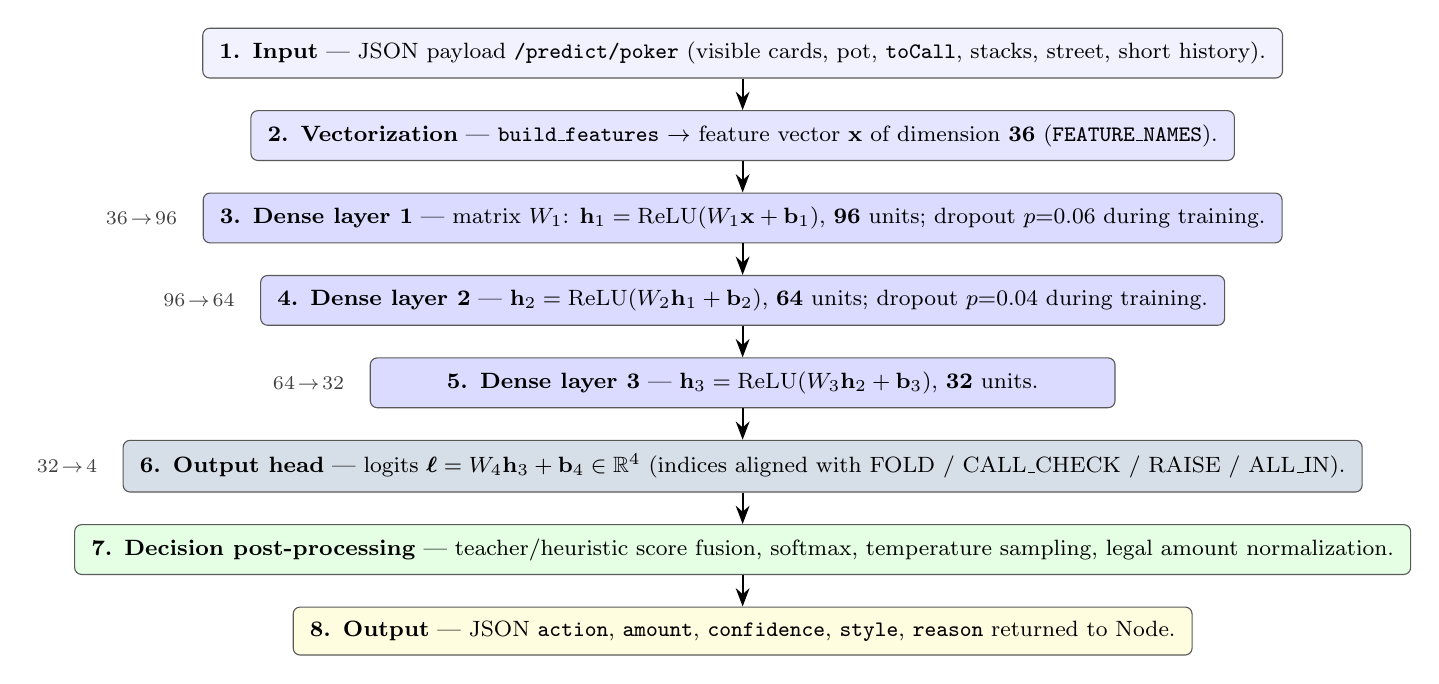
\begin{tikzpicture}[
  font=\footnotesize,
  >=Stealth,
  flow/.style={rectangle, draw=black!65, rounded corners=2.5pt, align=center, minimum width=0.78\textwidth, inner ysep=5pt, inner xsep=6pt},
  lab/.style={font=\scriptsize, text=black!75},
]
\node[flow, fill=blue!5] (n0) {\textbf{1. Input} — JSON payload \texttt{/predict/poker} (visible cards, pot, \texttt{toCall}, stacks, street, short history).};
\node[flow, fill=blue!10, below=4mm of n0] (n1) {\textbf{2. Vectorization} — \texttt{build\_features} $\rightarrow$ feature vector $\mathbf{x}$ of dimension \textbf{36} (\texttt{FEATURE\_NAMES}).};
\node[flow, fill=blue!14, below=4mm of n1] (n2) {\textbf{3. Dense layer 1} — matrix $W_1$: $\mathbf{h}_1 = \mathrm{ReLU}(W_1\mathbf{x}+\mathbf{b}_1)$, \textbf{96} units; dropout $p{=}0.06$ during training.};
\node[flow, fill=blue!14, below=4mm of n2] (n3) {\textbf{4. Dense layer 2} — $\mathbf{h}_2 = \mathrm{ReLU}(W_2\mathbf{h}_1+\mathbf{b}_2)$, \textbf{64} units; dropout $p{=}0.04$ during training.};
\node[flow, fill=blue!14, below=4mm of n3] (n4) {\textbf{5. Dense layer 3} — $\mathbf{h}_3 = \mathrm{ReLU}(W_3\mathbf{h}_2+\mathbf{b}_3)$, \textbf{32} units.};
\node[flow, fill=HeadingRule!16, below=4mm of n4] (n5) {\textbf{6. Output head} — logits $\boldsymbol{\ell}=W_4\mathbf{h}_3+\mathbf{b}_4 \in \mathbb{R}^{4}$ (indices aligned with FOLD / CALL\_CHECK / RAISE / ALL\_IN).};
\node[flow, fill=green!10, below=4mm of n5] (n6) {\textbf{7. Decision post-processing} — teacher/heuristic score fusion, softmax, temperature sampling, legal amount normalization.};
\node[flow, fill=yellow!12, below=4mm of n6] (n7) {\textbf{8. Output} — JSON \texttt{action}, \texttt{amount}, \texttt{confidence}, \texttt{style}, \texttt{reason} returned to Node.};
\draw[->, thick] (n0) -- (n1);
\draw[->, thick] (n1) -- (n2);
\draw[->, thick] (n2) -- (n3);
\draw[->, thick] (n3) -- (n4);
\draw[->, thick] (n4) -- (n5);
\draw[->, thick] (n5) -- (n6);
\draw[->, thick] (n6) -- (n7);
\node[lab, anchor=east, xshift=-2mm] at (n2.west) {$36\!\to\!96$};
\node[lab, anchor=east, xshift=-2mm] at (n3.west) {$96\!\to\!64$};
\node[lab, anchor=east, xshift=-2mm] at (n4.west) {$64\!\to\!32$};
\node[lab, anchor=east, xshift=-2mm] at (n5.west) {$32\!\to\!4$};
\end{tikzpicture}
}
\caption{Data flow through the expert MLP policy (\texttt{ExpertPolicy}): four successive linear transformations, \textbf{196} post-input neurons (96+64+32+4), then domain-specific post-processing before the HTTP response.}\label{fig:ai-mlp}
\end{figure}

\begin{figure}[htbp]
\centering
\resizebox{\linewidth}{!}{%
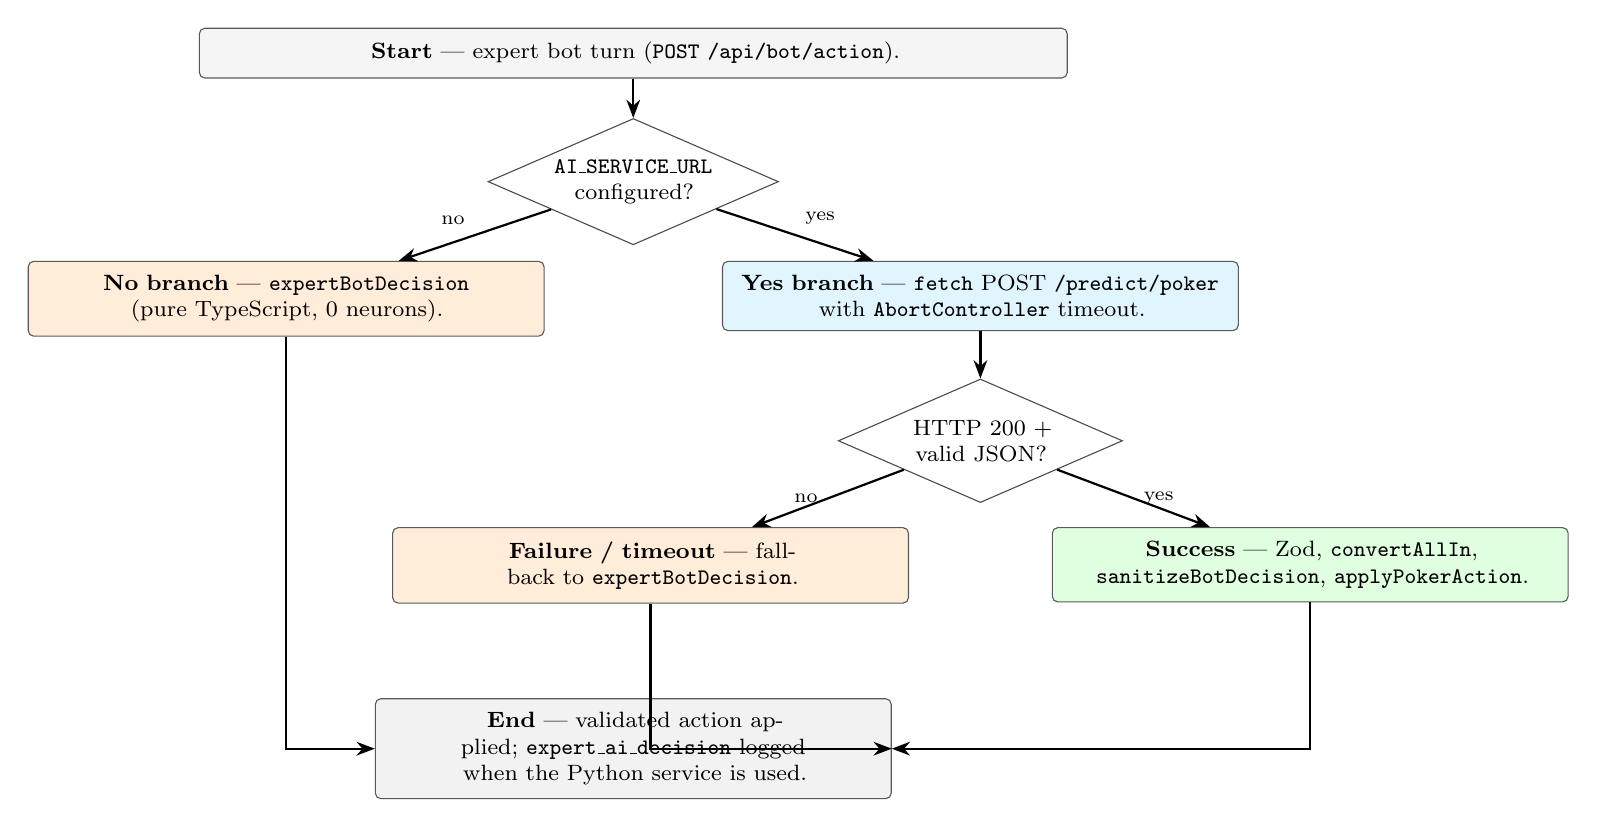
\begin{tikzpicture}[
  font=\footnotesize,
  >=Stealth,
  blk/.style={rectangle, draw=black!65, rounded corners=2pt, align=center, inner sep=5pt, text width=6.2cm},
  dia/.style={diamond, draw=black!70, aspect=2.3, inner sep=0pt, align=center, text width=2.4cm, minimum height=1.1cm},
]
\node[blk, fill=gray!8, text width=0.88\textwidth] (start) {\textbf{Start} — expert bot turn (\texttt{POST /api/bot/action}).};
\node[dia, below=5mm of start] (durl) {\textbf{\texttt{AI\_SERVICE\_URL}} configured?};
\node[blk, fill=orange!15, below left=6mm and 2mm of durl] (tsfb) {\textbf{No branch} — \texttt{expertBotDecision} (pure TypeScript, 0 neurons).};
\node[blk, fill=cyan!12, below right=6mm and 2mm of durl] (http) {\textbf{Yes branch} — \texttt{fetch} POST \texttt{/predict/poker} with \texttt{AbortController} timeout.};
\node[dia, below=6mm of http] (dok) {HTTP 200 + valid JSON?};
\node[blk, fill=orange!15, below left=7mm and 0mm of dok] (tsfb2) {\textbf{Failure / timeout} — fallback to \texttt{expertBotDecision}.};
\node[blk, fill=green!12, below right=7mm and 0mm of dok] (zod) {\textbf{Success} — Zod, \texttt{convertAllIn}, \texttt{sanitizeBotDecision}, \texttt{applyPokerAction}.};
\node[blk, fill=gray!10, below=12mm of durl |- tsfb2.south] (end) {\textbf{End} — validated action applied; \texttt{expert\_ai\_decision} logged when the Python service is used.};
\draw[->, thick] (start) -- (durl);
\draw[->, thick] (durl) -- node[above left, font=\scriptsize] {no} (tsfb);
\draw[->, thick] (durl) -- node[above right, font=\scriptsize] {yes} (http);
\draw[->, thick] (http) -- (dok);
\draw[->, thick] (dok) -- node[left, font=\scriptsize] {no} (tsfb2);
\draw[->, thick] (dok) -- node[right, font=\scriptsize] {yes} (zod);
\draw[->, thick] (tsfb) |- (end);
\draw[->, thick] (tsfb2) |- (end);
\draw[->, thick] (zod) |- (end);
\end{tikzpicture}
}
\caption{Node-side decision flow for the \texttt{expert} bot tier: optional Python service call, heuristic fallback, validation and action application.}\label{fig:ai-flow}
\end{figure}

\subsection{Use of AI assistants for code and documentation}

The team used modern AI assistants during the project as \textbf{support tools}, not as autonomous authors. On the engineering side, they helped generate first drafts of utility code, propose refactors, explain unfamiliar errors, compare implementation approaches and accelerate repetitive tasks such as type adjustments, test scaffolding or documentation cleanup. This was especially useful when working across several domains at once: poker logic, tournament orchestration, sockets, database models, deployment notes and report polishing.

AI assistants were also used for \textbf{text production and editing}. They helped restructure dense technical explanations, improve English phrasing, shorten repetitive sections, prepare appendix descriptions, and transform implementation notes into clearer academic prose. This support made the final report more readable, but the content remained based on the team's implementation, tests, diagrams and project decisions.

All AI-generated output was treated as \textbf{untrusted by default}. Code suggestions were reviewed by team members, adapted to the existing architecture, and validated through tests or manual checks before being kept. Text suggestions were edited to avoid overclaiming, remove unsupported statements, and preserve the academic context of the project. The team did not accept AI output when it contradicted server-side validation, security constraints, virtual-chip framing, or the actual behavior of the application.

\subsection{Enumerated uses of artificial intelligence}

The inventory below is exhaustive relative to the shipped codebase and this report's claims:

\begin{enumerate}
\item \textbf{TypeScript poker bots:} four handcrafted tiers (\texttt{easy}, \texttt{medium}, \texttt{hard}, \texttt{expert}) using normalized strength, pot geometry and tier-specific randomness (Appendix~\ref{app:bots}).
\item \textbf{Expert heuristic core:} \texttt{expertBotDecision} as the always-available policy when no remote model succeeds.
\item \textbf{Oracle / teaching path:} \texttt{expertOracleDecision} when opponent hole cards are known.
\item \textbf{Optional HTTP bot service:} FastAPI bundle under \path{ai-service}, endpoint \texttt{/predict/poker}, contract validated with Zod before any chip movement.
\item \textbf{Supervised PyTorch MLP:} \texttt{ExpertPolicy} plus \path{features.py} descriptors and teacher-driven labels (\path{expert_rules.py}, \path{decision.py}); weights serialised as \path{expert_bot.pt}; Figures~\ref{fig:ai-mlp}--\ref{fig:ai-flow}.
\item \textbf{Generative AI assistants (LLMs):} drafting/refactoring of application code, scripts and tests; restructuring and English polishing of internal notes and this report; never merged or submitted without human review and automated checks where applicable.
\end{enumerate}

\subsection{Limits and verification}

The \texttt{easy}/\texttt{medium}/\texttt{hard} tiers and the TypeScript \texttt{expert} fallback contain \textbf{no trainable neurons}: they are hand-crafted policies. Only the optional Python bundle instantiates the MLP in Figure~\ref{fig:ai-mlp}. Regardless of path, bot traffic is rate-limited, responses pass through Zod and sanitisation, and assistant-generated repository edits were never merged without human review and automated tests.

\section{Platform Functionalities}
\label{sec:functionalities}

Table~\ref{tab:inventory} lists major domains. Details appear only once, in the referenced appendix, to prevent duplication. \textbf{Appendices~\ref{app:map}--\ref{app:sources}} also record implemented formulas and structures: relational database model, closed-form \textbf{slot RTP} and unified \textbf{roulette RTP}, Monte Carlo equity with an error bound for the \textbf{Quantum HUD}, \textbf{Quantum Combi} exact probability plus its place in the hand-ranking cascade, \textbf{tournament bracket} sizing and RNG, and \textbf{code coverage} definitions.

{\small
\begin{longtable}{@{}p{2.0cm}p{3.8cm}p{4.8cm}p{2.6cm}@{}}
\caption{High-level functional inventory (representative surfaces).}\label{tab:inventory}\\
\toprule
Domain & User-visible capability & Primary UI entry & Deep dive \\
\midrule
\endfirsthead
\toprule
Domain & User-visible capability & Primary UI entry & Deep dive \\
\midrule
\endhead
Poker cash & Multiplayer tables, pot logic, chat, actions & \path{/game}, \path{/waiting-room} & Appendix~\ref{app:poker} \\
Poker bots & Practice tables, four difficulties & \path{/bot-configuration} & Appendix~\ref{app:bots} \\
HUD & Win chance and hand category estimates & In-game HUD & Appendix~\ref{app:hud} \\
Hidden bets & Side markets, pricing, settlement & In-game panel, \path{/results} & Appendix~\ref{app:hidden} \\
Blackjack & Solo + multi lobby/table & \path{/blackjack}, \path{/blackjack/lobby}, \path{/blackjack/table/:gameId} & Appendix~\ref{app:bj} \\
Casino & Slot and roulette & \path{/minigames} & Appendix~\ref{app:casino} \\
Tournaments & Waiting, play, results, winner side bets & \path{/tournaments/...} & Appendix~\ref{app:tournament} \\
Social & Friends, invites, loans & \path{/friends}, lobby flows & Appendix~\ref{app:social} \\
Progression & XP, badges, daily challenges, login streak, leaderboard & \path{/profile}, \path{/leaderboard} & Appendix~\ref{app:prog} \\
Account & Auth, 2FA, avatars, profile edit & \path{/auth}, \path{/edit-profile} & Appendix~\ref{app:auth} \\
Admin & Operator web console (JWT admin role) & \path{/admin/console} & Appendix~\ref{app:ops} \\
Ops & Metrics, health, CI, packaging & N/A (infra) & Appendix~\ref{app:ops} \\
Other UX & Gift codes, free recharge, post-game rating modal & Layout shell, lobby & Appendix~\ref{app:ops} \\
Feedback & User feedback and player reports & Lobby/settings flows & Appendix~\ref{app:ops} \\
Tournament UX & ZipRush mini-game while waiting & Tournament waiting screen & Appendix~\ref{app:tournament} \\
Demo & Example and deal teaching routes & \path{/game-example}, \path{/game-deal} & Appendix~\ref{app:poker} \\
A11y & Accessibility, table theming, ambient audio & Settings and table contexts & Appendix~\ref{app:map} \\
\end{longtable}
}

\subsection{Poker and Tournament System}
\label{sec:poker-tournament}

\subsubsection{Functional overview}

Poker is implemented with server-side rule enforcement: the client sends intentions, while the backend validates turns, blinds, raises, folds, pots, side pots and showdown results. Tournaments reuse this engine and add registration, fees, seeded brackets, table assignment, eliminations, rewards and winner side bets. Details are in Appendices~\ref{app:poker} and~\ref{app:tournament}.

Quantum Bluff also extends the standard Texas Hold'em ranking with an exclusive hand category: \textbf{Quantum Combi}. It is obtained when the seven available cards contain at least one 3, 5, 6, 7 and 10, regardless of suits. The ranks were chosen as a project signature: 3 refers to the third year of the Bachelor's degree, 6 to the sixth semester, 5 to the five letters of ``bluff'', and 7 to the seven letters of ``quantum''. The hand beats a flush but loses to a full house: this keeps the iconic premium hands of poker above the custom rule, while still making the project-specific combination strong enough to be visible and memorable in gameplay. The exact probability calculation and comparison with standard poker hands are given in Appendix~\ref{app:hud}.

\begin{itemize}
\item \textbf{Poker core}: backend table and cash-game controllers enforce legal actions and chip movement.
\item \textbf{Tournament orchestration}: dedicated tournament services create rounds, tables and transitions.
\item \textbf{Real time}: live events notify players about table assignment, next rounds, eliminations and completion.
\item \textbf{Reproducibility}: Mulberry32 + Fisher--Yates gives the same bracket for the same players and seed.
\end{itemize}

\subsubsection{Four-phase tournament lifecycle}

\begin{center}
\begin{tabular}{@{}p{3.5cm}p{9cm}@{}}
\toprule
\textbf{Phase} & \textbf{Activities} \\
\midrule
\texttt{REGISTRATION\_OPEN} & Players join and entry fees (10\% of stack) are deducted atomically. Fees accumulate into a centralized prize pool. Player state: \texttt{REGISTERED}. \\
\texttt{STARTING} & Bracket is generated deterministically. Player assignment is seeded and reproducible. Tables are dynamically sized (2--9 players each). Player state: \texttt{ACTIVE}. \\
\texttt{IN\_PROGRESS} & Multiple poker games execute concurrently at separate tables. Losers are eliminated and ranked. Winners advance to the next round. \\
\texttt{COMPLETED} & Final rankings determine XP rewards and prize distribution through atomic updates. \\
\bottomrule
\end{tabular}
\end{center}

\subsubsection{Multi-pot settlement: fairness under all-in}

The same side-pot logic is used in cash and tournament tables. If three players are all-in for 100, 150 and 200 chips, the pot is split into a main pot and side pots so that each player can only win chips they were eligible to contest:

\begin{enumerate}
\item Extract unique bet levels in sorted order: $\{100, 150, 200\}$.
\item For each level $\ell$, compute increment $\Delta_i = \ell_i - \ell_{i-1}$ and pool contribution $\Delta_i \times n_{\text{players}}$.
\item Distribute each pool only among players who contributed at that level.
\end{enumerate}

This deterministic splitting keeps all-in situations fair and testable. Implementation details are in Appendix~\ref{app:tournament}.

\subsubsection{Security and performance}

Entry fees, rewards and winner-bet settlements use atomic database updates. Action deduplication (\texttt{handId + actionId}) prevents duplicate mutations after retransmission. Snapshots support restart recovery, and table sizes adapt to player count (for example $[4,4]$ for 8 players and $[5,4]$ for 9 players). Appendix~\ref{app:tournament} gives the bracket arithmetic, RNG seeding and tournament flow diagram.

\subsection{Casino Games and AI Bot Integration}
\label{sec:casino-ai}

\subsubsection{Scope and functionality}

Beyond poker, Quantum Bluff integrates three casino games---blackjack (solo and multiplayer), European roulette (37-pocket wheel), and a three-reel slot machine---plus a four-tier AI bot system (easy, medium, hard, expert) for practice and entertainment. Each casino game is engineered with closed-form return-to-player (RTP) calculations: slots deliver $95.63\%$ RTP (house edge $4.37\%$), roulette delivers $97.297\%$ RTP (house edge $2.703\%$ per bet line), and blackjack approximates $99.3\%$ RTP under basic strategy. All outcomes are computed server-side, persisted to an immutable wallet ledger, and broadcast to clients via WebSocket; clients never ``decide'' results. Mathematical and implementation details appear in Appendices~\ref{app:bj}, \ref{app:casino}, \ref{app:bots}, and~\ref{app:rewards}.

The AI bot framework provides practice opponents across all four poker difficulty tiers. Bots participate in cash games (sit-and-go), tournament tables, and practice-only tables. They synthesize hand strength heuristics (normalized sigma), pot odds, stack pressure, and per-tier decision templates (bluff vs.\ value) to produce strategically coherent play. The expert tier optionally delegates to an external PyTorch model for advanced decision-making; on network failure, it gracefully reverts to the hard tier.

\subsubsection{Architecture: validation and live delivery}

The casino subsystem follows the same validation pattern as poker:

\begin{enumerate}
\item \textbf{Client submission}: player places a bet (blackjack, roulette, or slot spin) or bot decides action via WebSocket event (e.g.\ \texttt{PLACE\_ROULETTE\_BETS}, \texttt{SPIN\_SLOT}).
\item \textbf{Server validation}: backend validates bet size, balance sufficiency, and game state consistency atomically.
\item \textbf{Outcome computation}: the server uses injected RNG to draw the outcome (roulette pocket, slot symbols, blackjack card); for bots, it calls \texttt{decideBotAction} with normalized hand strength.
\item \textbf{Ledger recording}: a wallet ledger entry (\texttt{GAME\_WIN} or \texttt{GAME\_LOSS}) is created atomically with the balance update, capturing user ID, reason, amounts, and ISO timestamp.
\item \textbf{WebSocket broadcast}: outcome is emitted to the player's room (e.g.\ \texttt{ROULETTE\_RESULT \{ pocket, payouts \}}) so the client renders the result without delay.
\item \textbf{Snapshot persistence}: game state (dealer hand, final balances) is snapshotted to PostgreSQL for crash recovery.
\end{enumerate}

This keeps outcome and ledger updates tied together: in normal operation they commit together, or neither commit. Clients can place bets and observe results, but cannot force outcomes. The same settlement pattern is expanded in Appendix~\ref{app:rewards}.

\subsubsection{AI bot decision algorithm and complexity analysis}

The core of the bot framework is the \textbf{normalized hand strength} (sigma) computation and multi-tier decision dispatch. Let the bot's visible cards (two to seven) yield a raw hand evaluation score $H$ via \texttt{getHandValue}. The code normalizes to the unit interval:
\[
\sigma = \min\Bigl(1,\,\max\bigl(0,\,\frac{H}{S_{\max}}\bigr)\Bigr),
\quad
S_{\max} = 9 \cdot 15^5 + 14 \cdot 15^4,
\]
where $S_{\max}$ is the theoretical best hand (straight flush with top kickers). This ensures $\sigma \in [0, 1]$ regardless of the board texture or number of opponents. Appendix~\ref{app:bots} gives the tier-specific decision paths.

The bot then dispatches to a tier-specific decision function:
\[
\texttt{decideBotAction}(\sigma, \texttt{potOdds}, \texttt{stackPressure}, \text{tier}) \to \{\texttt{FOLD}, \texttt{CALL}, \texttt{CHECK}, \texttt{RAISE}\}
\]

Each tier has distinct complexity:
\begin{itemize}
\item \textbf{Easy}: compares $\sigma$ to a fixed threshold; injects naive bluffs with probability $p_{\text{bluff}} = 0.15$ on free streets. Complexity: $\mathbf{O(1)}$.
\item \textbf{Medium}: integrates pot odds $\text{callAmount} / (\text{potSize} + \text{callAmount})$; adjusts bluff frequency by position (button $p=0.20$, under-the-gun $p=0.08$). Complexity: $\mathbf{O(1)}$.
\item \textbf{Hard}: maintains opponent hand range estimates (map of recent action patterns). Decision compares $\sigma$ against estimated opponent strength distribution. Complexity: $\mathbf{O(n)}$ where $n \le 8$ (number of opponents).
\item \textbf{Expert}: HTTP POST to external model (\texttt{.../predict/poker}) with JSON payload (compact card encoding, street, stacks, position). Zod-validated response; timeout (default 2000\,ms) reverts to hard tier. Complexity: $\mathbf{O(1)}$ on the bot side (async); external model latency is hidden.
\end{itemize}

All tiers converge on the same sigma input, enabling principled interpolation from naive to advanced strategy. The hard tier's $O(n)$ opponent tracking is acceptable because $n$ is small (typical tables have 2--9 players).

\subsubsection{Integration with poker and tournaments}

Casino games are separate from the poker state machine but share the wallet ledger and user authentication. Bots can be inserted into poker cash games or tournament tables by specifying a difficulty tier at table creation. The same bot decision logic applies; the only difference is the hand context (hole cards, board, position) provided by the runtime.

Full algorithmic details, RTP derivations, and per-tier heuristics are provided in Appendix~\ref{app:bots} (Bot AI), Appendix~\ref{app:bj} (blackjack), and Appendix~\ref{app:casino} (slots and roulette).

\subsection{Rewards, Wallet, and Transactions}
\label{sec:rewards-banking}

\subsubsection{Scope and architecture}

The rewards and wallet system orchestrates chip circulation, XP progression, and peer-to-peer lending across poker, casino games, tournaments and social loans. All chip movements are recorded in a \textbf{wallet ledger} with SHA-256 integrity hashing, providing audit-style traceability for the virtual economy. Clients never compute balance changes; they request actions and receive confirmed outcomes. Ledger entry and balance update commit together, or neither commits. See Appendix~\ref{app:rewards} for persisted fields and settlement examples.

\subsubsection{Gamification: XP curves, levels, and badge unlocks}

Player progression is governed by accumulated experience points (XP) and a deterministic level curve. The core formula is:

\[
\text{XP threshold for level } L = 50 \cdot L \cdot (L - 1), \quad L \in \{1, 2, \ldots, 99\}
\]

XP is awarded per action: poker (12 XP/hand + 20 bonus on win), blackjack (5 XP + 10 bonus), roulette/slots (4 XP + 8--10 bonus), tournaments (500 / 400 / 300 / 50 XP for placement). Badge unlocks are level-driven (10 tiers: novice→legend). Effective betting limits scale by level to prevent new players from wagering excessively: slot max bet grows from 500 to 5000 chips as level increases (capped at 25). Appendix~\ref{app:prog} records the progression modules.

\subsubsection{Wallet ledger and atomic transactions}

Every chip movement---game win/loss, loan disbursement, loan repayment, tournament prize---creates an immutable \texttt{WalletLedgerEntry}. Fields include user, reason, amount, before/after balances, optional round identifier, integrity hash and settlement state. For a casino game, the sequence is: validate bet and balance, compute the outcome, then update chips and ledger together. This keeps the ledger and displayed balance aligned with the database source of truth; Appendix~\ref{app:rewards} lists the persisted fields.

\subsubsection{Tournament rewards and peer loans}

Tournament prize pools sum all entry fees (typically 10\% of initial stack). Winners receive the pool; all participants receive placement-based XP. Reward grants are idempotent via a \texttt{TournamentRewardLedger} unique constraint, enabling crash recovery. Peer-to-peer loans between friends specify a principal $P$ and repayment rate $r\% \in \{10, 15, \ldots, 50\}$. The system converts $r$ to an annual interest via a lookup table (e.g.\ 10\% repayment → 30\% interest). When the borrower wins chips, the server automatically diverts a slice to the lender: $\text{slice} = \min(\text{remaining due}, \lfloor \text{grossWin} \cdot (r/100) \rfloor)$, capped at the amount owed. Repayment is mandatory; the loan settles atomically. Constraints: borrower and lender must be friends, borrower can have at most one active loan, lender must have sufficient chips at acceptance, rate-limited to 40 operations per 10 minutes. Tournament reward details are in Appendix~\ref{app:tournament}; loan and ledger details are in Appendices~\ref{app:social} and~\ref{app:rewards}.

\subsubsection{Integration with daily challenges and login streaks}

Daily challenges and login streaks (separate modules in \path{dailyChallenges}, \path{dailyLogin}) award XP using the same \texttt{awardXp} function, feeding into the gamification bundle. Client displays these in \path{/profile} and \path{/leaderboard} routes. Appendix~\ref{app:prog} links the relevant modules.

\section{System Architecture}
\label{sec:architecture}

\subsection{Monorepo layout}

The repository splits into a Vite single-page frontend, an Express/Socket.IO backend, and a local PostgreSQL development database. The frontend bootstraps global providers and routes; the backend composes middleware, REST routes and the real-time gateway. Appendix~\ref{app:map} provides a compact subsystem overview.

\subsection{Central architectural model}

Quantum Bluff is organized around a \textbf{layered architecture}. The React client handles navigation, rendering, forms and immediate feedback. Gameplay decisions, casino outcomes, tournament progression, wallet movements, hidden-bet settlement and rewards are validated in backend services.

The backend is split into two entry surfaces. REST endpoints handle durable commands such as authentication, profile updates, wallet operations, tournament creation, social actions and history queries. The real-time gateway handles table joins, turn actions, sanitized snapshots, tournament assignments and presence updates. Both surfaces share JWT verification, role separation, suspension checks, rate limits and domain-level validation.

Behind these entry points, domain services isolate poker rules, blackjack, casino mini-games, tournaments, hidden bets, social features, rewards and wallet accounting. PostgreSQL stores durable state through Prisma; Redis supports short-lived runtime concerns such as token blacklist, rate limiting and distributed broadcasts. This separation keeps UI rendering, event routing, domain rules and persisted history distinct.

Appendix~\ref{app:architecture} provides the full architecture diagram; Appendix~\ref{app:db} shows the relational data model behind the persistence layer.

\subsection{Structured tournaments (outline)}

Multi-table Texas Hold'em tournaments are a \textbf{first-class server domain}: Prisma-backed registration and fees, a periodic scheduler that auto-starts due events, runtime orchestration that builds bracket rounds and assigns poker tables, deterministic table splitting and re-seating, winner-bet settlement, and boot-time recovery. The tournament UI binds waiting room, in-tournament play, results, and ZipRush. Exact bracket arithmetic, RNG seeding, and coverage metrics are in Appendices~\ref{app:tournament} and~\ref{app:coverage}.

\subsection{Real-time communication}
\label{sec:realtime}

Quantum Bluff uses live socket events for gameplay, lobby updates, invitations, tournament events and social notifications. The browser sends intentions; the backend validates identity, game state, turn order, chip balance and action legality before broadcasting any result.

Synchronization is based on private/shared channels and sanitized snapshots. On join or reconnect, the server sends a complete state view instead of relying only on incremental events, which avoids rebuilding a game from stale partial updates.

Confidentiality is handled in the same layer: seated players receive their own private cards, while other players and spectators receive sanitized views. Multi-instance delivery, table locking, reconnection behavior and security checks are detailed in Appendix~\ref{app:realtime}.

\subsection{Persistence and integrity}

Prisma models capture users, games, tournaments, loans, hidden bet tickets, wallet ledger rows and related data. Critical monetary flows favor short database transactions. Appendix~\ref{app:rewards} explains the ledger side of these models.

\subsection{Data model overview (Prisma)}

The persistence layer is relational PostgreSQL accessed through Prisma. Representative entities include: \texttt{User} (credentials, profile, chips, XP fields, avatar storage keys), \texttt{Game}/seat models for poker tables, \texttt{BlackjackRoom} and related seat/invitation models for multiplayer blackjack, tournament tables for bracket state and winner-bet tickets, \texttt{Friendship} and messaging hooks, loan and ledger tables for social/casino flows, and audit-friendly structures for wallet history. Full cardinality and migration history are summarized from the Prisma schema and migrations; a simplified relational model is provided in Appendix~\ref{app:db}, and domain usage is split across Appendices~\ref{app:poker}, \ref{app:bj}, \ref{app:tournament}, \ref{app:social}, \ref{app:prog}, and~\ref{app:rewards}.

\subsection{Diagram}

Figure~\ref{fig:flow} shows a \textbf{runtime flow diagram} (logical path, not deployment topology). Further architectural detail is consolidated in Appendices~\ref{app:map}, \ref{app:architecture}, and~\ref{app:realtime}.

\begin{figure}[htbp]
\centering
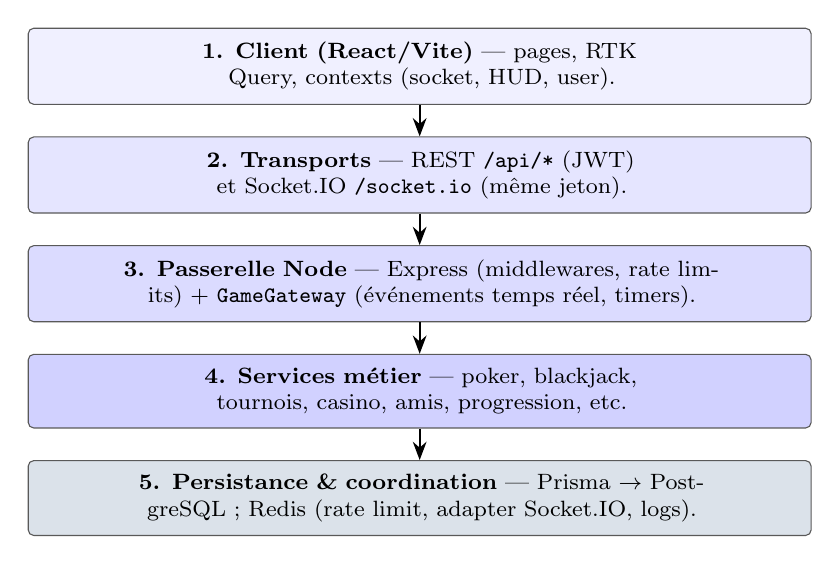
\begin{tikzpicture}[
  font=\footnotesize,
  >=Stealth,
  archstep/.style={rectangle, draw=black!65, rounded corners=2pt, align=center, inner sep=5pt, minimum width=0.82\textwidth, text width=0.76\textwidth},
]
\node[archstep, fill=blue!6] (c) {\textbf{1. Client (React/Vite)} — pages, RTK Query, contexts (socket, HUD, user).};
\node[archstep, fill=blue!10, below=4mm of c] (a) {\textbf{2. Transports} — REST \texttt{/api/*} (JWT) et Socket.IO \texttt{/socket.io} (même jeton).};
\node[archstep, fill=blue!14, below=4mm of a] (g) {\textbf{3. Passerelle Node} — Express (middlewares, rate limits) + \texttt{GameGateway} (événements temps réel, timers).};
\node[archstep, fill=blue!18, below=4mm of g] (s) {\textbf{4. Services métier} — poker, blackjack, tournois, casino, amis, progression, etc.};
\node[archstep, fill=HeadingRule!14, below=4mm of s] (p) {\textbf{5. Persistance \& coordination} — Prisma $\rightarrow$ PostgreSQL ; Redis (rate limit, adapter Socket.IO, logs).};
\draw[->, thick] (c) -- (a);
\draw[->, thick] (a) -- (g);
\draw[->, thick] (g) -- (s);
\draw[->, thick] (s) -- (p);
\end{tikzpicture}
\caption{Monorepo layers: client UI, REST/Socket.IO transports, Node gateway, domain services, PostgreSQL and Redis.}\label{fig:flow}
\end{figure}

\section{Deployment and operational runbook}
\label{sec:deploy}

\subsection{Local development stack}

The root development script launches PostgreSQL, a lightweight AI helper, the Node/Express server, and the Vite client under \texttt{concurrently}. Redis should be available for rate limiting, action logging, and the Socket.IO Redis adapter when exercising multi-instance paths. First-time setup, tester onboarding, and troubleshooting are consolidated in Appendix~\ref{app:ops}.

\subsection{Production and desktop delivery}

VM-oriented deployment (Node, PostgreSQL, Redis, PM2), environment files, and Electron auto-update mechanics are documented separately from the main report. The pipeline builds runnable \textbf{container images} on \texttt{develop}, \texttt{main}, and \texttt{release/*} using \textbf{Kaniko}. It authenticates to the GitLab registry, pushes immutable SHA-tagged images plus rolling aliases, and lets the VM pull validated images without rebuilding from source on the host. Reverse-proxy and deployment artefacts are summarized in Appendix~\ref{app:ops}.

\subsection{CI/CD pipeline and VM updates with GitLab Runner Shell mode}

The Quantum Bluff project uses a \textbf{multi-stage GitLab CI pipeline} configured for \textbf{five stages}: verify (linting and unit tests), test-security (npm audit and Trivy scanning), build (transpilation), docker-build (Kaniko image construction), and deploy (staging and production). Appendix~\ref{app:ops} records the CI/ops entry points, while Appendix~\ref{app:coverage} defines coverage metrics.

\subsubsection{Five pipeline stages}

\paragraph{1. Verify:} On \texttt{develop} and \texttt{main} branches, \textbf{backend:verify} runs Jest tests with coverage in a PostgreSQL 15 service; \textbf{frontend:verify} runs Vitest on the client; \textbf{database:test} smoke-tests the database. On \texttt{feature/*} and \texttt{fix/*} branches, \textbf{backend:lint} performs lightweight linting only.

\paragraph{2. Test-Security:} \textbf{security:npm} audits lockfiles for high/critical vulnerabilities; \textbf{security:trivy} scans the filesystem with Trivy (skipping \texttt{node\_modules}, \texttt{dist}, platform folders). Both allow failure to avoid blocking deployments.

\paragraph{3. Build:} On \texttt{main} and \texttt{release/*}, \textbf{backend:build} generates the Prisma client and transpiles the backend; \textbf{frontend:build} bundles the Vite/React application into static production assets.

\paragraph{4. Docker-Build:} Kaniko builds three images: \textbf{docker:build} (backend tagged \texttt{:latest}), \textbf{docker:build:client} (frontend tagged \texttt{:client-latest} with \texttt{VITE\_API\_URL} build argument), and \textbf{docker:build:ai-service} (Python service, release/* only). All images are pushed to the GitLab Container Registry.

\paragraph{5. Deploy:} \textbf{deploy:staging} automatically runs on \texttt{develop}; \textbf{deploy:production} requires manual approval on \texttt{main}.

\subsubsection{GitLab Runner in Shell mode: pull-based deployment agent}

The key deployment improvement is a \textbf{GitLab Runner} installed directly on the deployment VM, configured in \textbf{Shell executor mode}. This reduces manual deployment work while respecting the firewall constraint: the university's strict inbound policy blocks external connections to the VM. The Runner uses a \textbf{pull-based polling mechanism}:

\begin{enumerate}
\item \textbf{Polling:} Every 3 seconds, the Runner queries GitLab: "Are there new commits on \texttt{develop} or \texttt{main}?" instead of waiting for GitLab to push notifications inbound.
\item \textbf{Tag-based routing:} The deploy jobs in \texttt{.gitlab-ci.yml} use the tag \texttt{runner-vm-quantum}, telling GitLab: "Only the Runner with this tag can execute these jobs." This ensures the job stays in the queue until the VM's Runner claims it.
\item \textbf{Shell executor:} The Runner is configured with executor type \texttt{shell}, executing scripts directly on the VM. Docker socket access is granted via \texttt{sudo usermod -aG docker gitlab-runner}.
\end{enumerate}

\subsubsection{Automated deployment sequence}

When the Runner claims a deploy job, it executes the shell script sequentially:

\begin{enumerate}
\item \textbf{Docker authentication:} CI injects registry credentials; the job runs \texttt{docker login} against \texttt{\$CI\_REGISTRY} (password via stdin) before pulls.
\item \textbf{Dynamic .env generation:} Reconstructs \texttt{.env} from secure GitLab variables (\texttt{\$JWT\_SECRET}, \texttt{\$DATABASE\_URL}), ensuring secrets never exist in source code.
\item \textbf{Hot pull and restart:} \texttt{docker compose pull} fetches latest images, then \texttt{docker compose up -d --force-recreate} recreates containers with reduced manual downtime.
\item \textbf{Database migrations:} \texttt{npx prisma migrate deploy} applies schema changes automatically inside the backend container.
\end{enumerate}

\subsubsection{Automated updates and reduced manual intervention}

The \texttt{--force-recreate} flag on \texttt{docker compose up} tears down and recreates containers from freshly pulled images. The result is \textbf{automated deployment}: every \texttt{git push} to \texttt{develop} can stage code quickly, while production deployment on \texttt{main} still requires manual approval. The Runner polls for work, retrieves encrypted secrets from GitLab, and applies updates within the VM's local context, reducing the need for manual SSH sessions, cron jobs or webhook proxies. Operational fallbacks and Redis-related constraints are referenced in Appendix~\ref{app:ops}.

\subsubsection{Further reading}

See Appendix~\ref{app:ops} for the CI, deployment and production container references.

\subsection{Electron and Capacitor artefacts}

Quantum Bluff was designed as a \textbf{multi-platform application} without maintaining separate native clients. The web version remains the reference target; the same React/TypeScript interface is then packaged through \textbf{Electron} for desktop systems and \textbf{Capacitor} for mobile shells. This strategy keeps authentication, lobby, poker tables, tournaments, casino games, friends, profile, rewards and administration screens consistent across environments, while all accounts, chip balances, history and social data remain centralized on the backend.

The same React UI is built under three Vite modes: default web, \texttt{--mode electron}, and \texttt{--mode capacitor}. \textbf{Electron} targets \textbf{Windows} (NSIS $\rightarrow$ \texttt{.exe} installer), \textbf{macOS} (\texttt{.dmg} / signed artefacts per builder defaults), and \textbf{Linux} (\texttt{AppImage} and \texttt{.deb}). Published updates are served from a generic update URL for \texttt{electron-updater}.

\textbf{Capacitor} wraps the static build for \textbf{iOS} and \textbf{Android}. \texttt{npm run build:cap} creates the mobile-oriented web build, and \texttt{npm run cap:sync} copies it into the native projects. Mobile WebViews require extra care around backend URLs, socket origins and CORS because they may run from origins such as \texttt{capacitor://localhost}; the backend therefore includes native WebView origins in its allowed deployment configuration. Dedicated packaging scripts support course delivery builds.

\begin{table}[htbp]
\centering
\scriptsize
\setlength{\tabcolsep}{3pt}
\begin{tabular}{@{}p{2.5cm}p{3.4cm}p{3.2cm}p{4.2cm}@{}}
\toprule
Target & Main command & Generated artefact & Main configuration area \\
\midrule
Web & \texttt{npm run build} & Static Vite build & Vite frontend configuration \\
Windows desktop & \texttt{npm run electron:build:win} & NSIS \texttt{.exe} installer & Electron Builder configuration \\
macOS desktop & \texttt{npm run electron:build:mac} & macOS app / \texttt{.dmg} & Electron Builder configuration \\
Linux desktop & \texttt{npm run electron:build:linux} & \texttt{AppImage} and \texttt{.deb} & Electron Builder configuration \\
Android & \texttt{npm run cap:android} & Android Studio project / APK via Gradle & Capacitor Android project \\
iOS & \texttt{npm run cap:ios} & Xcode project / archive & Capacitor iOS project \\
\bottomrule
\end{tabular}
\caption{Build targets for the web, desktop and mobile versions of Quantum Bluff.}\label{tab:platform-builds}
\end{table}

The benefit is consistency and maintainability: a poker table fix, tournament UI change or profile improvement is implemented once in the React codebase and then reused across web, desktop and mobile packaging targets. The limitation is release engineering overhead: desktop signing, update publication, Android Studio/Xcode builds, WebView behavior and platform-specific network configuration still require dedicated validation. Appendix~\ref{app:ops} lists the npm entry points.

\section{Security, Testing and Stability}
\label{sec:security}

\subsection{Authentication and anti-cheat}

Security is implemented as defence in depth. Short-lived JWT access tokens identify users on REST and Socket.IO paths; protected routes reject malformed, revoked, admin-role, missing-user or suspended-account tokens. Passwords are hashed with bcrypt, validated with Zod rules, and optional TOTP 2FA is available for stronger account protection.

Anti-cheat controls are applied at several levels. HTTP middleware checks bans and suspicious account patterns; the real-time gateway validates that a socket cannot act as another player; gameplay helpers detect abnormal action bursts; and moderation features persist reports and blocked-user relationships. Rate limits, CORS/Helmet configuration, idempotency for sensitive mutations and separated admin access complete the security baseline.

The result is a coherent academic prototype security model: identity is checked repeatedly, gameplay remains server-side, and suspicious behavior is logged or refused. The detailed token flow, socket identity checks, rate limits and anti-cheat mechanisms are provided in Appendices~\ref{app:auth}, \ref{app:realtime}, and~\ref{app:ops}.

\subsection{Testing and debugging}

Broad automated coverage exists on the server and focused frontend modules. Browser smoke tests and manual multiplayer scenarios complement unit tests for flows that depend on sockets, multiple users or real-time timing. Appendix~\ref{app:coverage} explains how test and coverage numbers are interpreted.

\subsection{Automated test inventory and CI (reference snapshot)}

Table~\ref{tab:tests} reflects a \textbf{May~2026} backend Jest run and frontend Vitest run. Coverage definitions are in Appendix~\ref{app:coverage}.

\begin{table}[htbp]
\centering
\small
\begin{tabular}{@{}lccc@{}}
\toprule
Layer & Runner & Test files / suites & Tests passed \\
\midrule
Backend & Jest & 51 & 520 \\
Frontend & Vitest & 13 & 83 \\
\midrule
\textbf{Total unit/integration} & --- & 64 & \textbf{603} \\
\bottomrule
\end{tabular}
\caption{Automated unit and integration test inventory (May~2026 snapshot).}\label{tab:tests}
\end{table}

\subsection{Code coverage policy (server)}

Jest collects coverage only on \textbf{logic-heavy backend paths}: poker/tournament bracket utilities, validation helpers and selected shared utilities; some monolithic controllers are excluded so the metric tracks maintainable units. \textbf{Global thresholds} require at least $80\%$ lines, statements, and functions, and $65\%$ branches, or CI fails. Table~\ref{tab:coverage} shows the latest measured aggregate on that scope. Appendix~\ref{app:coverage} defines the coverage ratios and relates them to tournament bracket tests.

\begin{table}[htbp]
\centering
\small
\begin{tabular}{@{}lcccc@{}}
\toprule
Layer & Lines & Statements & Functions & Branches \\
\midrule
Server (Jest scoped paths) & 86.56\% & 83.69\% & 88.75\% & 67.90\% \\
\midrule
Required minimum (threshold) & 80.00\% & 80.00\% & 80.00\% & 65.00\% \\
\bottomrule
\end{tabular}
\caption{Server Jest coverage aggregate on \texttt{collectCoverageFrom} (May~2026; \texttt{npm run test:coverage} on the backend).}\label{tab:coverage}
\end{table}

\noindent
\textbf{Client:} frontend validation should not be read from the raw Vitest global percentage alone. The May~2026 full-tree Vitest coverage remained low because most screens depend on sockets, browser APIs, multiple users and live API state; those flows were instead checked through browser smoke tests, manual poker/tournament scenarios and integration validation. Focused Vitest files still cover isolated frontend utilities, while the future target is to expand Playwright coverage for the main user journeys.

\noindent
GitLab CI encodes build and test gates for merge requests; the \texttt{docker-build} stage uses \textbf{Kaniko} for reproducible, rootless image builds pushed to the GitLab Container Registry. CI operational detail is in Appendix~\ref{app:ops}.

\subsection{Performance and stability}

Distributed socket delivery, structured logging, Prometheus metrics, readiness endpoints and graceful shutdown hooks support stability. See Appendices~\ref{app:realtime} and~\ref{app:ops}.

\section{Technical Challenges}
\label{sec:challenges}

\textbf{Concurrency around shared tables:} poker and blackjack runtimes use locking strategies to prevent split-brain chip mutations. Related runtime details appear in Appendices~\ref{app:poker}, \ref{app:bj}, and~\ref{app:realtime}.

\textbf{Recovery after process restarts:} blackjack and tournament subsystems implement recovery services invoked at boot; see Appendices~\ref{app:bj}, \ref{app:tournament}, and~\ref{app:realtime}.

\textbf{Hidden bet settlement coupling:} market resolution must align with poker street transitions; implemented in hidden-bet resolver modules (Appendix~\ref{app:hidden}).

\textbf{Internationalization without clobbering user preference:} guest screens force English using \texttt{react-i18next} with a fixed \texttt{lng: 'en'} override so the global language stored for authenticated use is unchanged; see Appendix~\ref{app:auth}.

\subsection{Implemented solutions}

The project was completed by decomposing the platform into domain modules while keeping one consistent runtime architecture: React for presentation, Express for REST APIs, sockets for live state, PostgreSQL for durable data, and Redis for runtime coordination. This avoids a single monolithic ``game page'' and lets poker, blackjack, casino mini-games, tournaments, social features and progression evolve under one validation model. The module map is in Appendix~\ref{app:map}.

The most important implementation choice was to keep gameplay, chip movement and settlement on the server. Poker clients only send intentions; poker, hidden bets, tournaments, casino outcomes, rewards and peer loans are validated by domain services before any balance or ledger mutation is committed. Reconnection is handled through room-based events plus full sanitized snapshots, so clients can recover from missed WebSocket events without reconstructing private state themselves. See Appendices~\ref{app:poker}, \ref{app:hidden}, \ref{app:tournament}, and~\ref{app:realtime}.

The same pattern applies to extended modules: casino games have dedicated services; tournaments separate registration, assignment, progression and rewards; social features combine persistence with notifications; progression and daily rewards remain backend-validated. Security layers HTTP middleware, socket authentication, gateway checks, rate limits, idempotency and anti-cheat alerts. Monetary integrity relies on short database transactions and immutable ledger entries. Further detail is moved to Appendix~\ref{app:implemented-solutions}.

Finally, the project added validation and test coverage around these solutions: schema tests for authentication, integration tests for waiting-room identity trust, and gateway tests for authenticated real-time snapshots. The remaining improvements would be a formal threat model, broader end-to-end coverage and a polished observability dashboard; measurable targets are listed in Section~\ref{sec:limitations}. Appendix~\ref{app:coverage} gives the coverage definitions.

\section{Ethics, privacy, and academic integrity}
\label{sec:ethics}

\subsection{Virtual economy and regulatory framing}

Quantum Bluff uses \textbf{in-game virtual chips} for learning and demonstration. It is not a licensed real-money gambling operator; features that resemble casino products are implemented in an \textbf{academic engineering} context and should be evaluated as software artefacts, not as a commercial gaming offer. The casino payout models are documented in Appendix~\ref{app:casino}.

\subsection{Personal data}

Accounts store identifiers needed for authentication and gameplay (email, username, hashed password, optional TOTP secrets, profile metadata). Operators deploying a public instance must align hosting, retention, and breach notification with applicable law (including GDPR for EU users). This report does not replace a data protection impact assessment. Appendix~\ref{app:auth} lists the account/profile surfaces.

\subsection{Integrity of authorship and AI assistance}

Section~\ref{sec:ai} states how large language models were used as drafting assistants. All merged code remained subject to human review, tests, and repository governance. The contribution statements in Section~\ref{sec:contributions} summarize the declared responsibilities of the team members for the final report.

\section{Individual Contributions}
\label{sec:contributions}

\noindent\textit{Each member narrative below is capped at roughly half a printed page to match the programme guideline on individual statements.}

\subsection{Omar -- project management and architecture alignment}

Organizational narrative: Section~\ref{sec:management}. I coordinated \textbf{cross-cutting delivery}: distributed live play, rate limiting, alignment between schema migrations and gameplay features, and risk reviews before widening scope (tournaments, casino modules, loans), together with the technical lead's sequencing of gateway and recovery work.

I drove the backend \textbf{automated coverage} objective toward the programme expectation ($\sim$80\%): prioritising tests on weak modules and blocking ``coverage debt'' merges before final validation (Section~\ref{sec:security}, Appendix~\ref{app:coverage}).

\subsection{Massi -- DevOps Infrastructure, Real-Time Networking, and Cross-Platform Delivery}

I focused on \textbf{Socket.IO} behaviour (reconnection, timeouts, client wiring), production topology (\textbf{Nginx}, Docker isolation, PostgreSQL/Redis boundaries, GitLab Runner Shell deployments), and \textbf{Electron} packaging including Windows installers. I contributed to stabilisation around cross-origin issues, chat inputs and live state drift alongside reproducible migrations and restarts.

\subsection{Yigit -- Debugging, Quality Assurance and Gameplay Stability}

I concentrated on \textbf{QA} across multiplayer poker, tournaments and responsive layouts: reproducing defects, validating fixes without regressions, and stressing tournament transitions (showdown, automatic next hand, final table). I reported mobile UI problems (overlapping controls, chip readability, table/toolbar spacing), helped tune responsive layouts, and supported merge-request reviews plus pre-release playtests.

\subsection{Azra -- Backend Modeling, Visual Design and User Experience Features}

I modelled \textbf{game entities} and card logic on the backend, contributed to \textbf{tournament} configuration and rules, and produced visual assets (cards; roulette/slot surfaces) for a coherent casino identity. I improved \textbf{accessibility} (colour-blind mode), fixed responsive issues on multiplayer screens, and shipped retention-oriented UX (daily login rewards, recharge helpers, promotional codes) with testing through stabilisation.

\subsection{Linda -- Security, Real-Time Features and UI/UX}

I implemented \textbf{security-sensitive} paths (JWT and socket auth, password/admin protections, rate limits, anti-cheat alerts) alongside gameplay routes, blinds and waiting-room fixes. I delivered \textbf{social features} end-to-end (friends, lobby chat, invitations, blocks, reports, notifications, blocked-room warnings) across REST and sockets.

On the \textbf{frontend}, I polished lobby/profile/table layouts, blackjack/roulette/mini-games, settings and audio; I resolved merge conflicts, repaired CI regressions, assisted PDF/report finalisation and ran repeated end-to-end validation before delivery.

\subsection{Mohamed -- Technical Leader}

As \textbf{technical lead} I coordinated multiplayer UX (animations, rounds, pot updates), \textbf{tournament} delivery alongside the PM during stabilisation, and early visual specs for mini-games. I shipped \textbf{anti-cheat/moderation} pieces (IP-based multi-account hints, reaction-time heuristics, global bans, secured admin APIs), configured the production VM, tightened \textbf{CORS} and rate limits, wired \textbf{CI/CD} deployment automation, and contributed retention systems (daily rewards, cooldowns) validated through live tournament sessions.

\subsection{Abdoulaye -- Database Architecture, Backend Integration and Stabilization}

I owned \textbf{PostgreSQL/Prisma} evolution (migrations, indexing, ERD, waiting-room and friend models, statistics/game history), Docker DB setup, seeds/backups and discussions on separating auth/game data for resilience. I integrated login/register flows, poker lobby/table surfaces, accessibility/audio/table preferences, and coordinated beta validation across web, Electron and Capacitor with documentation updates.

\subsection{Soheil -- Backend Support and Testing}

I supported backend validation through targeted reviews, regression hunts during integration and gameplay/API debugging; contribution breadth was intentionally smaller than feature owners but reinforced reliability before delivery.

\subsection{Contribution summary table}

The table below summarizes the expanded contribution narratives and links them to representative technical areas in the repository.

\begin{table}[htbp]
\centering
\small
\begin{tabular}{@{}p{2.6cm}p{4.6cm}p{5.8cm}@{}}
\toprule
Member & Primary areas (self-declared) & Verifiable artefacts (commits, MRs, modules) \\
\midrule
Linda & Security, network, deployment safeguards, CI/CD review & See narrative above; security hardening, real-time social features, UI/UX polish and final validation \\
Abdoulaye & Database architecture, Prisma, backend integration, stabilization & See narrative above; schema evolution, migrations, ERD, waiting-room/friend relations, testing, deployment preparation and cross-platform validation \\
Soheil & Backend support, selected reviews, tests and debugging & See narrative above; backend validation support, regression checks and final stabilization assistance \\
Mohamed & Technical leadership, multiplayer UX, tournaments, security, deployment & See narrative above; UI finalization, tournament system, anti-cheat/moderation, production VM and CI/CD deployment workflows \\
Massi & DevOps infrastructure, WebSocket networking, Nginx routing, Docker/CI, Electron packaging & See narrative above; Socket.IO integration, deployment configuration, CI/CD automation, Electron packaging and stabilization work \\
Azra & Backend modeling, card/game logic, visual design, accessibility, UX features & See narrative above; work around game entities, card logic, mini-game interfaces, accessibility and reward/recharge flows \\
Yigit & Debugging, QA, tournaments, responsive UI, Git/MR reviews & See narrative above; playtests on poker tables, tournaments, mobile layouts and deployment regressions \\
\bottomrule
\end{tabular}
\caption{Individual contributions: expanded statements appear as subsections above and are summarized here by primary technical area.}\label{tab:contrib}
\end{table}

\section{Limitations and Future Work}
\label{sec:limitations}

\subsection{Current limitations}

\begin{itemize}
\item \textbf{Documentation volume vs.\ examiners' time:} internal generated reports are useful as indexes but are not all human-curated line-by-line.
\item \textbf{Dual loader providers:} two frontend entry layers both wrap \texttt{LoaderProvider}; harmless but confusing---should be deduplicated.
\item \textbf{Packaging surface area:} Electron/Capacitor increase release engineering work (signing, store policies) beyond the core web path; see Appendix~\ref{app:ops}.
\item \textbf{External identity and banking integrations:} the project does not include Google account verification, real email/SMS one-time-code delivery, real payment cards, or real bank account connections. These features require certified third-party providers, compliance checks, payment/banking approvals, and stronger legal safeguards than were available in the academic project context. The implementation therefore uses simulated top-ups, virtual chips, and internal authentication flows rather than real financial instruments.
\end{itemize}

\subsection{Future improvements}

The next improvements are intentionally scoped as measurable increments rather than open-ended wishes. \textbf{Person-days (pd)} denote one contributor focused for a full day; ranges assume familiarity with the repo and include review buffer.

\begin{itemize}
\item \textbf{End-to-end testing:} add 8--10 Playwright scenarios (login, room creation, poker table, tournament, blackjack, reward claim), targeting roughly \textbf{+15\% critical-flow coverage}; \textbf{$\sim$8--12\,pd} spread over about two calendar weeks with parallel lectures.
\item \textbf{Recovery and observability (real-time):} Grafana-style dashboards plus exported \textbf{live metrics} (tournament queue depth, socket failures, wallet mutation errors). Targets: incident triage \textbf{under 5 minutes} and \textbf{first automated alert within 60 seconds} on configured thresholds (Redis adapter health, scheduler backlog); \textbf{$\sim$6--10\,pd} including instrumentation.
\item \textbf{Multi-instance deployment (Socket.IO scaling):} validate \textbf{three nodes} with sticky sessions and distributed fan-out; measurable exit criteria: \textbf{zero dropped gameplay events} on the reference load profile, \textbf{client re-association under 3 seconds} after node failover, and \textbf{P95 socket latency overhead $\leq$20\,\%} versus a single instance; \textbf{$\sim$10--15\,pd}.
\item \textbf{Gameplay synchronisation and latency:} budget the path \emph{validated poker action $\rightarrow$ subscriber emission} for \textbf{P95 $\leq$150\,ms} under a documented synthetic load (6--10 seats per table), and \textbf{state catch-up after reconnect $\leq$2\,s} under nominal conditions; \textbf{$\sim$5--8\,pd} (profiling, queues, payload sizing).
\item \textbf{Tournament capacity:} load-test registration and scheduler paths toward \textbf{$\geq$20 concurrently active tournaments} \emph{or} \textbf{$\geq$500 cumulative open registrations}, while keeping \textbf{scheduler drift bounded to $\leq$60\,s} outside declared maintenance windows; \textbf{$\sim$8--12\,pd}.
\item \textbf{Test coverage (measurable uplift):} complement UI journeys with \textbf{+10 percentage-points} of server \emph{branch} coverage on tournament/socket/wallet modules versus the last archived snapshot, \emph{or} sustain \textbf{$\geq$85\,\%} branches on those folders; \textbf{$\sim$6--10\,pd}.
\item \textbf{Tournament analytics:} KPI endpoints/UI (round duration, bust order, table wait, winner-bet volume); \textbf{$\sim$6--10\,pd} from existing tables and ledger events.
\item \textbf{Technical debt (loader duplication):} collapse the dual \texttt{LoaderProvider} shells; \textbf{$\sim$0.5--1\,pd}.
\item \textbf{Certified identity/payment providers:} calendar dominated by provider onboarding and compliance; once contracts exist, \textbf{$\sim$15--25\,pd} for OAuth/OIDC flows, SMS OTP wiring and PCI-scoped payment stubs---excluding legal review and audits.
\end{itemize}

\begin{table}[htbp]
\centering
\small
\begin{tabular}{@{}p{6.4cm}p{6.8cm}@{}}
\toprule
Theme & Indicative engineering effort \\
\midrule
Playwright critical journeys & 8--12 person-days \\
Observability + real-time alerting & 6--10 person-days \\
Multi-instance Socket.IO (measured SLOs) & 10--15 person-days \\
Gameplay sync / latency budgets & 5--8 person-days \\
Tournament capacity (load + scheduler bounds) & 8--12 person-days \\
Targeted branch coverage (tournament/socket/wallet) & 6--10 person-days \\
Tournament KPI surfaces & 6--10 person-days \\
Loader/provider deduplication & 0.5--1 person-day \\
Certified ID / payments (post-vendor) & 15--25 person-days + external compliance \\
\bottomrule
\end{tabular}
\caption{Rough effort envelope for future improvements (Section~\ref{sec:limitations}); estimates are planning aids, not quotations.}\label{tab:future-effort}
\end{table}

The related starting points are Appendices~\ref{app:ops}, \ref{app:bots}, \ref{app:tournament}, \ref{app:auth}, and~\ref{app:user-guide}.

\section{Conclusion}

Quantum Bluff exceeded its initial poker-only charter by integrating multiple casino modes, tournaments, social lending, progression systems, and operational hardening while keeping a monorepo with clear separation between UI, API, and game logic. The project demonstrates that a student team can approach industry-like constraints---real-time state, monetary integrity, security, and observability---when management explicitly trades early waterfall rigidity for controlled agile iteration. The appendix set acts as the technical index for these domains, especially Appendices~\ref{app:poker}--\ref{app:ops}.

Lessons retained for similar efforts: (1)~anchor scope changes to \textbf{recoverable increments} (feature flags, migrations, recovery jobs); (2)~treat generated documentation as \textbf{hypotheses} until cross-read against code; (3)~keep \textbf{security and idempotency} on the critical path rather than as end-of-project polish.

\clearpage
\phantomsection
\section*{Acknowledgements}
\addcontentsline{toc}{section}{Acknowledgements}

\noindent
The team thanks \textbf{Jason Golda} for academic supervision of this L3 capstone, the University of Strasbourg Computer Science faculty for the project framework, the open-source maintainers of the libraries listed in Section~\ref{sec:tools}, and peers who provided feedback during playtests.

\appendix
\clearpage

\section{Repository map and routing}
\label{app:map}

\subsection{Programmed routing and shell}

Client routes are declared in \path{App.tsx}: public splash and auth (\path{/}, \path{/auth}, \path{/auth/admin}); authenticated gameplay and hub routes under \path{ProtectedRoute} with \path{Layout} (lobby, poker, blackjack, tournaments, mini-games, profile, friends, admin console). Admin routes use \path{AdminProtectedRoute}. Global providers stack in \path{main.tsx} (error boundary, loader, Redux, toasts, user, socket, Quantum HUD, hidden bets, audio) with an additional nested loader/invitation shell in \path{App.tsx}. Server REST mounts, rate-limit tiers, and health/metrics endpoints are wired in \path{index.ts}. A narrative overview also exists in \path{ARCHITECTURE.md}.

\section{Architecture diagram}
\label{app:architecture}

\subsection{Layered runtime architecture}

Figure~\ref{fig:appendix-architecture} summarizes the logical architecture used by Quantum Bluff. The important design rule is separation of responsibility: the client renders and sends intentions; the backend authenticates, validates and applies rules; domain services execute game and economy logic; PostgreSQL and Redis provide durable state and coordination.

\begin{figure}[htbp]
\centering
\resizebox{\textwidth}{!}{%
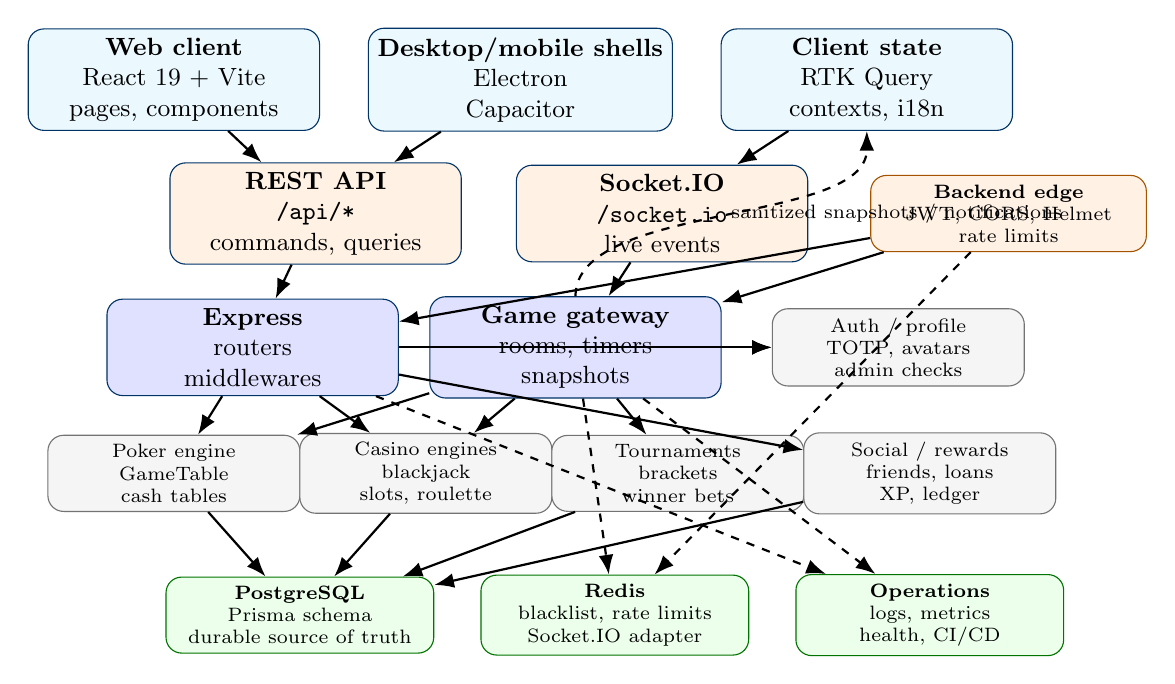
\begin{tikzpicture}[
  x=1cm,
  y=1cm,
  box/.style={
    rectangle,
    rounded corners=2mm,
    draw=HeadingRule,
    fill=blue!5,
    align=center,
    minimum width=3.7cm,
    minimum height=1.0cm,
    font=\small
  },
  svc/.style={
    rectangle,
    rounded corners=2mm,
    draw=black!55,
    fill=gray!8,
    align=center,
    minimum width=3.2cm,
    minimum height=0.9cm,
    font=\scriptsize
  },
  data/.style={
    rectangle,
    rounded corners=2mm,
    draw=green!45!black,
    fill=green!8,
    align=center,
    minimum width=3.4cm,
    minimum height=0.95cm,
    font=\scriptsize
  },
  guard/.style={
    rectangle,
    rounded corners=2mm,
    draw=orange!65!black,
    fill=orange!10,
    align=center,
    minimum width=3.5cm,
    minimum height=0.9cm,
    font=\scriptsize
  },
  arrow/.style={-{Latex[length=2.5mm]}, thick},
  event/.style={-{Latex[length=2.5mm]}, thick, dashed}
]

% Row 1: client surface
\node[box, fill=cyan!8] (web) at (0,0) {\textbf{Web client}\\React 19 + Vite\\pages, components};
\node[box, fill=cyan!8] (desktop) at (4.4,0) {\textbf{Desktop/mobile shells}\\Electron\\Capacitor};
\node[box, fill=cyan!8] (state) at (8.8,0) {\textbf{Client state}\\RTK Query\\contexts, i18n};

% Row 2: transport and edge
\node[box, fill=orange!10] (rest) at (1.8,-1.7) {\textbf{REST API}\\\texttt{/api/*}\\commands, queries};
\node[box, fill=orange!10] (socket) at (6.2,-1.7) {\textbf{Socket.IO}\\\texttt{/socket.io}\\live events};
\node[guard] (edge) at (10.6,-1.7) {\textbf{Backend edge}\\JWT, CORS, Helmet\\rate limits};

% Row 3: gateway and domain services
\node[box, fill=blue!12] (express) at (1.0,-3.4) {\textbf{Express}\\routers\\middlewares};
\node[box, fill=blue!12] (gateway) at (5.1,-3.4) {\textbf{Game gateway}\\rooms, timers\\snapshots};
\node[svc] (auth) at (9.2,-3.4) {Auth / profile\\TOTP, avatars\\admin checks};

\node[svc] (poker) at (0,-5.0) {Poker engine\\GameTable\\cash tables};
\node[svc] (casino) at (3.2,-5.0) {Casino engines\\blackjack\\slots, roulette};
\node[svc] (tournaments) at (6.4,-5.0) {Tournaments\\brackets\\winner bets};
\node[svc] (social) at (9.6,-5.0) {Social / rewards\\friends, loans\\XP, ledger};

% Row 4: data and infrastructure
\node[data] (pg) at (1.6,-6.8) {\textbf{PostgreSQL}\\Prisma schema\\durable source of truth};
\node[data] (redis) at (5.6,-6.8) {\textbf{Redis}\\blacklist, rate limits\\Socket.IO adapter};
\node[data] (ops) at (9.6,-6.8) {\textbf{Operations}\\logs, metrics\\health, CI/CD};

\draw[arrow] (web) -- (rest);
\draw[arrow] (desktop) -- (rest);
\draw[arrow] (state) -- (socket);
\draw[arrow] (rest) -- (express);
\draw[arrow] (socket) -- (gateway);
\draw[arrow] (edge) -- (express);
\draw[arrow] (edge) -- (gateway);
\draw[arrow] (express) -- (auth);
\draw[arrow] (gateway) -- (auth);
\draw[arrow] (express) -- (poker);
\draw[arrow] (gateway) -- (poker);
\draw[arrow] (express) -- (casino);
\draw[arrow] (gateway) -- (casino);
\draw[arrow] (gateway) -- (tournaments);
\draw[arrow] (express) -- (social);
\draw[arrow] (poker) -- (pg);
\draw[arrow] (casino) -- (pg);
\draw[arrow] (tournaments) -- (pg);
\draw[arrow] (social) -- (pg);
\draw[event] (edge) -- (redis);
\draw[event] (gateway) -- (redis);
\draw[event] (express) -- (ops);
\draw[event] (gateway) -- (ops);
\draw[event] (gateway.north) .. controls +(0,1.2) and +(0,-1.2) .. node[right, font=\scriptsize]{sanitized snapshots / notifications} (state.south);
\end{tikzpicture}%
}
\caption{Layered architecture diagram: UI shells and client state, REST/Socket.IO transport, backend edge controls, domain services, PostgreSQL persistence, Redis coordination and operational monitoring.}
\label{fig:appendix-architecture}
\end{figure}

\subsection{Reading the diagram}

\begin{itemize}
\item \textbf{Client layer}: renders the lobby, tables, profiles and modals; it caches state but does not decide outcomes or balances.
\item \textbf{Transport layer}: REST carries durable commands and queries; Socket.IO carries low-latency gameplay and notification events.
\item \textbf{Backend edge}: applies JWT identity, role separation, CORS/Helmet, rate limits and request validation before domain code runs.
\item \textbf{Domain layer}: poker, blackjack, casino, tournament, social and reward services enforce rules and prepare database mutations.
\item \textbf{Infrastructure layer}: PostgreSQL stores durable state, Redis coordinates short-lived distributed concerns, and operational hooks expose health, metrics and deployment feedback.
\end{itemize}

\section{Relational database model}
\label{app:db}

\subsection{Relational mode and source of truth}

Quantum Bluff uses a \textbf{relational PostgreSQL database} accessed through Prisma. The authoritative schema is \path{schema.prisma}; migrations define the concrete SQL evolution. The central entity is \texttt{User}. Most gameplay, wallet, social, tournament and security tables reference it through foreign keys, which keeps identity, chip movements and audit history normalized instead of duplicating user information inside each feature.

\begin{figure}[htbp]
\centering
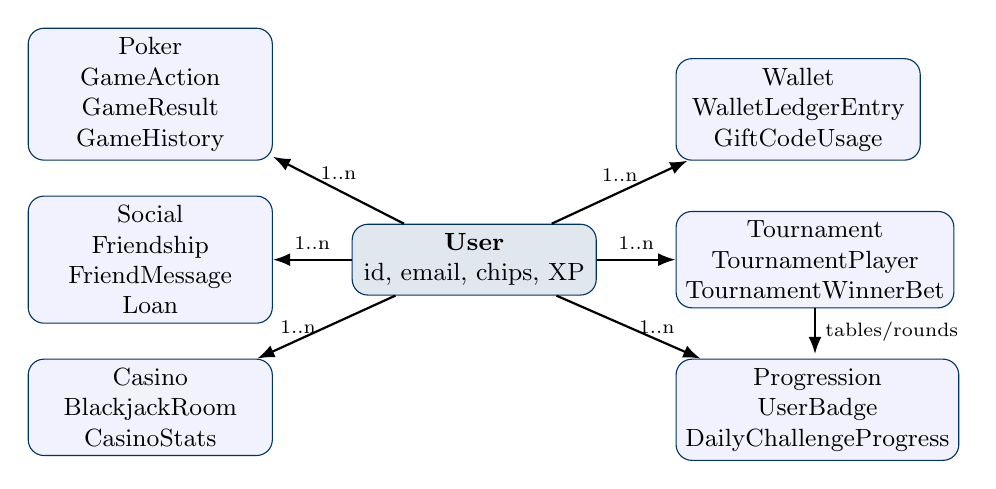
\begin{tikzpicture}[
  node distance=8mm and 10mm,
  ent/.style={
    rectangle,
    rounded corners=2mm,
    draw=HeadingRule,
    fill=blue!5,
    align=center,
    minimum width=3.1cm,
    minimum height=8mm,
    font=\small
  },
  rel/.style={-{Latex[length=2.2mm]}, thick}
]
\node[ent, fill=HeadingRule!12] (user) {\textbf{User}\\id, email, chips, XP};
\node[ent, above left=of user] (poker) {Poker\\GameAction\\GameResult\\GameHistory};
\node[ent, above right=of user] (wallet) {Wallet\\WalletLedgerEntry\\GiftCodeUsage};
\node[ent, left=of user] (social) {Social\\Friendship\\FriendMessage\\Loan};
\node[ent, right=of user] (tournament) {Tournament\\TournamentPlayer\\TournamentWinnerBet};
\node[ent, below left=of user] (casino) {Casino\\BlackjackRoom\\CasinoStats};
\node[ent, below right=of user] (progress) {Progression\\UserBadge\\DailyChallengeProgress};

\draw[rel] (user) -- node[above, font=\scriptsize]{1..n} (poker);
\draw[rel] (user) -- node[above, font=\scriptsize]{1..n} (wallet);
\draw[rel] (user) -- node[above, font=\scriptsize]{1..n} (social);
\draw[rel] (user) -- node[above, font=\scriptsize]{1..n} (tournament);
\draw[rel] (user) -- node[left, font=\scriptsize]{1..n} (casino);
\draw[rel] (user) -- node[right, font=\scriptsize]{1..n} (progress);
\draw[rel] (tournament) -- node[right, font=\scriptsize]{tables/rounds} ++(0,-1.2);
\end{tikzpicture}
\caption{Simplified relational model: \texttt{User} is the central parent for gameplay, wallet, social, tournament, casino and progression data.}
\label{fig:db-relational-model}
\end{figure}

\subsection{Main relational groups}

\begin{longtable}{@{}p{3.1cm}p{5.35cm}p{5.95cm}@{}}
\caption{Main relational groups in the Prisma schema.}\label{tab:db-relational-groups}\\
\toprule
Domain & Main tables & Relation pattern \\
\midrule
\endfirsthead
\toprule
Domain & Main tables & Relation pattern \\
\midrule
\endhead
Identity and profile & \texttt{User}, \texttt{UserStats}, \texttt{PlayerStats}, \texttt{CasinoStats} & One user owns optional 1--1 profile/stat rows and many gameplay records. \\
Poker & \texttt{GameHistory}, \texttt{GameAction}, \texttt{GameResult}, \texttt{WaitingRoom}, \texttt{RoomPlayer} & Users join rooms, perform actions, and appear in result/history rows. \\
Tournament & \texttt{Tournament}, \texttt{TournamentPlayer}, \texttt{TournamentRound}, \texttt{TournamentTable}, \texttt{TournamentWinnerBet} & A tournament has many players, rounds and tables; winner bets link a bettor user to a predicted winner user. \\
Wallet and rewards & \texttt{WalletLedgerEntry}, \texttt{TournamentRewardLedger}, \texttt{GiftCode}, \texttt{GiftCodeUsage} & Each chip-changing operation creates auditable rows tied to a user and reason. \\
Social and loans & \texttt{Friendship}, \texttt{FriendRequest}, \texttt{FriendMessage}, \texttt{LoanRequest}, \texttt{Loan}, \texttt{LoanRepayment} & User-to-user relations are modeled through explicit join tables and named Prisma relations. \\
Casino and blackjack & \texttt{BlackjackRoom}, \texttt{BlackjackRoomSeat}, \texttt{BlackjackRoomSnapshot}, \texttt{CasinoStats} & Rooms have seats and snapshots; casino statistics remain attached to the user. \\
Hidden bets & \shortstack[l]{\texttt{HiddenBetTicket}\\\texttt{HiddenBetSelection}\\\texttt{HiddenBetHandResolution}} & A ticket belongs to a user and game/hand, with child selection rows and resolution records. \\
\bottomrule
\end{longtable}

\section{Poker engine and cash game}
\label{app:poker}

\subsection{What was programmed}

Authoritative table logic lives in \path{GameTable.ts} (seats, streets, pot and side pots, action legality, showdown ordering) and \path{CashGameController.ts} (chip debits/credits, transitions between phases). Hand evaluation and category ordering use \path{Evaluator.ts}. Real-time delivery and timers (e.g.\ \texttt{TURN\_TIMER} with 20\,s auto-fold/check) are implemented in \path{game.gateway.ts} together with anti-cheat hooks. The client implements presentation and input in \path{Game.tsx} and reusable components under \path{components} (\texttt{PokerTable}, \texttt{ActionButtons}, \texttt{CommunityCards}, chat, HUD hooks). \textbf{All wagering state changes are validated and applied on the server}; the client never ``decides'' the winner.

\subsection{Rules enforced}

Texas Hold'em flow from blinds through preflop, flop, turn, river, and showdown; fold, check, call, raise semantics; minimum raise increments; side pots when players are all-in for different amounts. Waiting-room creation and join flows are handled by dedicated routes (\path{waitingRoom.routes.ts}, \path{game.api.routes.ts}) coordinated with the gateway.

\subsection{Further reading}

Structured logic notes: \path{01_poker_moteur.md}, \path{02_cashgame_controller.md}.

\section{Bot AI and practice integration}
\label{app:bots}

\subsection{Programmed pipeline}

Figures~\ref{fig:ai-mlp} and~\ref{fig:ai-flow} in the main report depict the optional PyTorch policy ($36\to96\to64\to32\to4$, \textbf{196} post-input units, \textbf{11\,972} trainable scalars in the linear stack) and the Node/Python pipeline. This appendix keeps the algebraic detail for heuristics and oracle mode. \texttt{POST /api/bot/action} (\path{bot.routes.ts}) validates difficulty and cards, then calls \path{botAI.ts}. Practice tables chain bot turns through \path{practiceBotTurns.service.ts}; HTTP orchestration and optional expert delegation sit in \path{botAi.service.ts}. Four difficulties are supported: \texttt{easy}, \texttt{medium}, \texttt{hard}, \texttt{expert}.

\subsection{Strength signal and decisions}

Let $H$ be the scalar hand score returned by \texttt{getHandValue} for the bot's visible cards (two to seven cards). The code normalizes
\[
\sigma = \min\Bigl(1,\,\max\bigl(0,\, H/S_{\max}\bigr)\Bigr),
\qquad
S_{\max} = 9\cdot 15^{5} + 14\cdot 15^{4},
\]
matching the encoding used by \path{Evaluator.ts}. Each difficulty combines $\sigma$ with pot odds (\texttt{callAmount}, \texttt{potSize}), heads-up vs.\ multiway flags, and pseudo-random draws to return \texttt{FOLD}, \texttt{CALL}, \texttt{CHECK}, or \texttt{RAISE} with an optional raise amount (chips rounded via \path{intChips}). The easy tier, for example, injects naive bluffs on a free street with fixed probability and biases calls when facing small bets with medium strength.

\subsection{Dispatch surface}

\texttt{decideBotAction} in \path{botAI.ts} switches on \texttt{difficulty} and routes to \texttt{easyBotDecision}, \texttt{mediumBotDecision}, \texttt{hardBotDecision}, or \texttt{expertBotDecision}. The HTTP layer (\path{botAi.service.ts}) may intercept \texttt{expert} to call an external model first.

\subsection{Decision dispatch and bot tier routing}

The function \texttt{decideBotAction}(\texttt{sigma}, \texttt{potOdds}, \texttt{stackPressure}, \texttt{difficulty}) accepts the normalized hand strength and situation parameters, then switches to the appropriate tier:
\begin{verbatim}
decideBotAction(sigma, potOdds, stackPressure, difficulty) {
  switch (difficulty) {
    case 'easy': return easyBotDecision(sigma, potOdds);
    case 'medium': return mediumBotDecision(sigma, potOdds, stackPressure);
    case 'hard': return hardBotDecision(sigma, potOdds, stackPressure);
    case 'expert': return expertBotDecision(...);
  }
}
\end{verbatim}
Each function returns \texttt{FOLD}, \texttt{CALL}, \texttt{CHECK}, or \texttt{RAISE} with an optional raise amount. For the expert tier, the HTTP layer (\path{botAi.service.ts}) may intercept and call an external model first; on timeout or failure, it reverts to hard tier.

\subsection{Bot tier specifics and complexity}

\paragraph{Easy tier.}
Strategy: fixed bluff probability on free streets (check or bet with zero cost to call); calls liberally with $\sigma \ge 0.3$. Decision logic: \texttt{if } $\sigma >$ \texttt{threshold, return RAISE; else FOLD}. Complexity: $\mathbf{O(1)}$ constant-time decision.

\paragraph{Medium tier.}
Strategy: integrates pot odds into sigma; compares $\sigma$ to the call-to-pot ratio $\texttt{callAmount} / (\texttt{potSize} + \texttt{callAmount})$. Bluff frequency adjusts by position (button more aggressive at $p_{\text{bluff}} = 0.20$; under the gun more conservative at $p = 0.08$). Complexity: $\mathbf{O(1)}$ constant-time.

\paragraph{Hard tier.}
Strategy: adds opponent hand range tracking; maintains a map of recent player actions (check, call, raise) to infer strength ranges. Decision compares $\sigma$ against estimated opponent strength distribution via weighted averages. Complexity: $\mathbf{O(n)}$ where $n \le 8$ is the number of tracked opponents (typical tables have 2--9 players).

\paragraph{Expert tier.}
Strategy: delegates to external PyTorch model via HTTP POST. Payload includes compact card encoding, current street, stacks, pot size, and position. Fallback to hard tier if service unavailable or timeout (default 2000\,ms). Complexity: $\mathbf{O(1)}$ on the bot side (HTTP call is async); external model inference latency is hidden from the decision.

\subsection{Expert tier: optional Python service}

When \texttt{AI\_SERVICE\_URL} is configured, \path{botAi.service.ts} issues \texttt{POST .../predict/poker} with a JSON payload built by \texttt{buildAiPayload} (compact card encoding, street, stacks, pot, position, optional opponent holes for oracle debugging). The JSON body is validated through \texttt{aiResponseSchema} (Zod): allowed actions include \texttt{ALL\_IN}, which is lowered to a legal \texttt{RAISE}/\texttt{CALL}/\texttt{FOLD} via \texttt{convertAllIn}. Timeouts use \texttt{AbortController} and \texttt{env.aiServiceTimeoutMs}; structured logs record \texttt{expert\_ai\_decision} with latency and style. Any failure reverts to \texttt{expertBotDecision}.

\subsection{Expert oracle path (TypeScript, no network)}

For revealed opponent holes, \texttt{expertOracleDecision} compares normalized strengths. Hero strength is
\[
\sigma_{\mathrm{hero}}=\texttt{normalizedHandStrength}(\text{hero},\text{board}).
\]
For each known opponent hole pair the service obtains $\sigma_i$, then sorts $\sigma_{(1)}\ge\cdots\ge\sigma_{(n)}$. If $n\le 2$, set $S_{\mathrm{opp}}=\sigma_{(1)}$. If $n\ge 3$, \texttt{compositeOpponentNormalizedStrength} combines extremes via
\[
S_{\mathrm{opp}} = w\,\sigma_{(1)} + (1-w)\,\sigma_{(\lfloor n/2\rfloor)},
\qquad
w = \min\bigl(0.68,\,\max\bigl(0.35,\,0.56 - 0.05\,(n-3)\bigr)\bigr),
\]
so the policy blends the strongest visible villain with a median-like opponent instead of assuming everyone holds the nuts. The edge $\Delta=\sigma_{\mathrm{hero}}-S_{\mathrm{opp}}$ is compared to pot odds and stack pressure ratios built from \texttt{callAmount}, \texttt{potSize}, and \texttt{playerChips} to emit stylised lines (\texttt{value}, \texttt{bluff}, \texttt{pot\_control}, \texttt{discipline}, etc.).

\subsection{Further reading}

Design notes: \path{IA_EXPERT_BOT.md}.

\section{Probabilities, Quantum HUD, and Monte Carlo helper}
\label{app:hud}

\subsection{Division of responsibilities}

The \textbf{Quantum HUD} (\path{QuantumHUD.tsx}, context \path{QuantumHUDContext.tsx}) displays \textit{estimates} for the authenticated player. These are computed client-side for responsiveness and are \textbf{not} used to settle real-money outcomes (the product uses virtual chips). Server-side hidden-bet pricing uses separate tabular services (Appendix~\ref{app:hidden}).

\subsection{Monte Carlo equity estimator}

Implementation file: \path{pokerMonteCarloEquity.ts}. Let $N$ be the number of iterations (default $N=2000$, constant \texttt{MONTE\_CARLO\_DEFAULT\_ITERATIONS}). For each iteration the code:
\begin{enumerate}
\item Builds the remaining deck excluding hero and community cards (helper \texttt{buildDeckExcluding}).
\item Draws, without replacement, the missing board cards and $2\times n_{\mathrm{opp}}$ opponent hole cards using a partial Fisher--Yates swap sampler (\texttt{drawWithoutReplacement}).
\item Evaluates the hero and each opponent seven-card hand with \texttt{evaluateSevenEval} (same taxonomy as the server evaluator).
\item Splits the simulated pot equally among all players that achieve the best score.
\end{enumerate}
If $S_t \in \{0, 1/k\}$ is the hero's share on iteration $t$ when $k$ players tie for the best score, the reported equity is
\[
\hat{e} = \frac{1}{N}\sum_{t=1}^{N} S_t .
\]
A histogram of category indices (0--9) is accumulated in parallel for UX badges.

\subsection{Monte Carlo error budget (HUD analogue to RTP)}

The HUD does \textbf{not} implement a house-banked game: there is no monetary \textbf{RTP} in the casino sense. The quantity $\hat{e}$ is an \textbf{equity} estimate (expected share of the pot at showdown under uniform completion of unknown cards). If $e$ denotes the true value of that expectation under the model, then $\mathrm{E}[\hat{e}]=e$ (each draw is independent and fair with respect to the remaining deck). Because $0\le S_t\le 1$,
\[
\mathrm{Var}(S_t)\le \frac{1}{4},
\qquad
\mathrm{Var}(\hat{e})=\frac{\mathrm{Var}(S_t)}{N},
\qquad
\mathrm{SE}(\hat{e})\le \frac{1}{2\sqrt{N}}.
\]
With the shipped default $N=2000$, $\mathrm{SE}(\hat{e})\le 1/(2\sqrt{2000})\approx 0.01118$ (about $1.1$ equity points at most in the worst-case variance bound).

\subsection{Quantum Combi---exact enumeration formula}

The promotional ``Quantum Combi'' category (documented for players in \path{QUANTUM_COMBI.adoc}) requires ranks $\{3,5,6,7,10\}$ each to appear \textbf{at least once} among the seven cards (two private + five community). All $\binom{52}{7}$ seven-card subsets are equally likely:
\[
\binom{52}{7} = 133784560 .
\]
For each rank $r$ in that set, let $A_r$ be the event ``no card of rank $r$ among the seven''; then $|A_r|=\binom{48}{7}$. By the principle of inclusion--exclusion over five ranks,
\[
\Bigl|\bigcup_{r} A_r\Bigr|
  = \sum_{k=1}^{5} (-1)^{k+1}\binom{5}{k}\binom{52-4k}{7}
  = 133002736 .
\]
Hence the favourable count is $133784560-133002736 = 781824$ and
\[
P(\text{Quantum Combi}) = \frac{781824}{133784560} \approx 0.00584 \approx 0.584\%.
\]

\subsection{Seven-card hand probabilities and ranking context}

The standard seven-card Texas Hold'em frequencies are computed over the same denominator $\binom{52}{7}=133\,784\,560$. Table~\ref{tab:seven-card-probabilities} gives the classical distribution before introducing the project-specific Quantum Combi rule.

\begin{table}[htbp]
\centering
\small
\begin{tabular}{@{}lrr@{}}
\toprule
Hand category & Seven-card combinations & Probability \\
\midrule
Straight flush & 41\,584 & 0.0311\% \\
Four of a kind & 224\,848 & 0.1681\% \\
Full house & 3\,473\,184 & 2.5961\% \\
Flush & 4\,047\,644 & 3.0255\% \\
Straight & 6\,180\,020 & 4.6194\% \\
Three of a kind & 6\,461\,620 & 4.8299\% \\
Two pair & 31\,433\,400 & 23.4955\% \\
One pair & 58\,627\,800 & 43.8225\% \\
High card & 23\,294\,460 & 17.4119\% \\
\bottomrule
\end{tabular}
\caption{Classical seven-card poker hand frequencies used as the probability context for positioning the custom Quantum Combi category.}\label{tab:seven-card-probabilities}
\end{table}

The raw Quantum Combi condition has probability $0.584\%$, which is rarer than a classical flush and also rarer than a full house. Its final position in the game is therefore a \textbf{design decision}, not a strict rarity-only ordering. The team placed it \textbf{above flush} so that the exclusive project hand has meaningful value, but \textbf{below full house} to preserve the familiar hierarchy of premium poker hands and avoid making a rank-set novelty override one of the most recognizable traditional combinations.

\subsection{Quantum Combi in the hand-ranking ladder (server and HUD)}

Both \path{Evaluator.ts} and \path{pokerHandCategory.ts} use the same \textbf{best-of-seven} cascade. Categories are integers $0$ (high card) through $9$ (straight flush); a larger packed score beats a smaller one. After ruling out straight flush ($9$), four-of-a-kind ($8$), and full house ($7$), the code tests \textbf{Quantum Combi before flush or straight}. Quantum applies iff every rank in $\{3,5,6,7,10\}$ appears at least once in the seven rank values (Ace is coded as $14$). If two players both make Quantum Combi, the tie-break compares the two remaining kickers after removing one 3, one 5, one 6, one 7 and one 10. Let $V$ be the multiset of those seven values; subtract one occurrence of each mandatory rank; sort the remaining values descending and take the top two as kickers $(\kappa_1,\kappa_2)$. The score is
\[
\texttt{packScore}(6,\kappa_1,\kappa_2) = 6\cdot 15^{5} + \kappa_1\cdot 15^{4} + \kappa_2\cdot 15^{3},
\]
padding unused kicker slots with zeros in the implementation. Only if Quantum fails does the evaluator continue to flush ($5$), straight ($4$), three-of-a-kind, two pair, one pair, high card. Thus Quantum is positioned \textbf{strictly between full house and flush}, as a design choice documented in \path{QUANTUM_COMBI.adoc}.

\section{Hidden betting system}
\label{app:hidden}

\subsection{Programmed architecture}

Hidden side markets are implemented under \path{hiddenBets}: typed markets and snapshots (\path{markets.ts}, \path{types.ts}), pricing tables (\path{pricingTables.ts}, \path{pricingTables.v1.ts}), live heuristics (\path{livePricing.ts}), quote and placement services, ledger context, and street-aware resolvers (\path{hiddenBetResolver.ts}). HTTP routes are mounted in \path{hiddenBets.routes.ts}.

\subsection{Odds and tables (example)}

Live markets use tabulated decimal odds keyed by table parameters. For instance, function \path{oddsPlayerWinsCurrentHand}\linebreak maps the number of active players $n\in[2,9]$ to a fixed grid (e.g.\ $n=2 \rightarrow 1.9$, $n=5 \rightarrow 3.0$, $n=9 \rightarrow 4.6$); companion functions cover showdown vs.\ fold endings. These values are \textbf{heuristic} prices distanced from the pre-hand model (see code comments \texttt{hidden-bets-live-v1}), not Monte Carlo outputs from the HUD.

\subsection{Further reading}

\path{HIDDEN_BETS_SPEC.md}, \path{07_hidden_bets_moteur.md}.

\section{Tournaments and winner side bets}
\label{app:tournament}

\subsection{Tournament system diagram}

\begin{figure}[htbp]
\centering
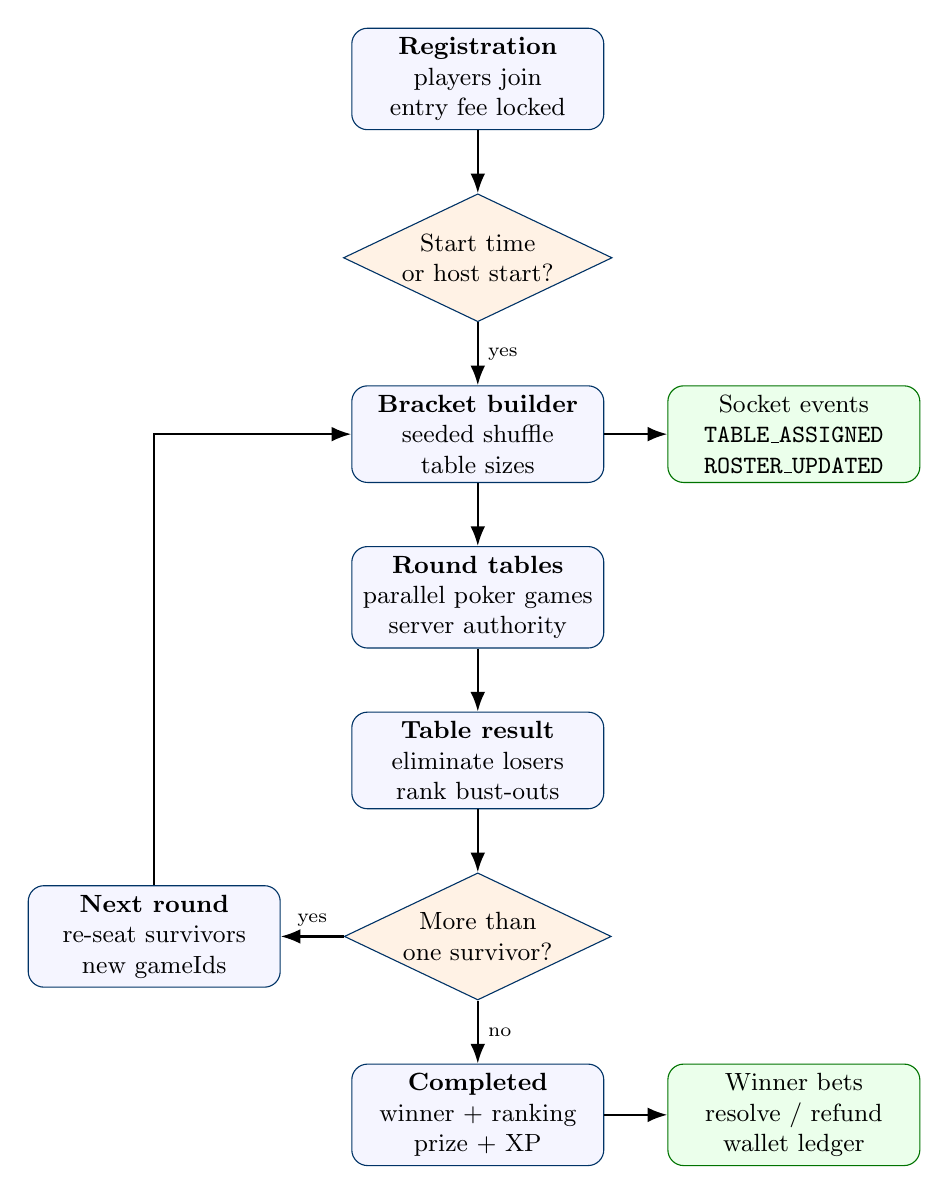
\begin{tikzpicture}[
  node distance=8mm and 8mm,
  flow/.style={
    rectangle,
    rounded corners=2mm,
    draw=HeadingRule,
    fill=blue!4,
    align=center,
    minimum width=3.2cm,
    minimum height=9mm,
    font=\small
  },
  decision/.style={
    diamond,
    aspect=2.1,
    draw=HeadingRule,
    fill=orange!10,
    align=center,
    inner sep=1pt,
    font=\small
  },
  event/.style={
    rectangle,
    rounded corners=2mm,
    draw=green!45!black,
    fill=green!8,
    align=center,
    minimum width=3.2cm,
    minimum height=9mm,
    font=\small
  },
  arrow/.style={-{Latex[length=2.5mm]}, thick}
]
\node[flow] (reg) {\textbf{Registration}\\players join\\entry fee locked};
\node[decision, below=of reg] (ready) {Start time\\or host start?};
\node[flow, below=of ready] (bracket) {\textbf{Bracket builder}\\seeded shuffle\\table sizes};
\node[event, right=of bracket] (assign) {Socket events\\\texttt{TABLE\_ASSIGNED}\\\texttt{ROSTER\_UPDATED}};
\node[flow, below=of bracket] (tables) {\textbf{Round tables}\\parallel poker games\\server authority};
\node[flow, below=of tables] (settle) {\textbf{Table result}\\eliminate losers\\rank bust-outs};
\node[decision, below=of settle] (survivors) {More than\\one survivor?};
\node[flow, left=of survivors] (next) {\textbf{Next round}\\re-seat survivors\\new gameIds};
\node[flow, below=of survivors] (complete) {\textbf{Completed}\\winner + ranking\\prize + XP};
\node[event, right=of complete] (bets) {Winner bets\\resolve / refund\\wallet ledger};

\draw[arrow] (reg) -- (ready);
\draw[arrow] (ready) -- node[right, font=\scriptsize]{yes} (bracket);
\draw[arrow] (bracket) -- (tables);
\draw[arrow] (bracket) -- (assign);
\draw[arrow] (tables) -- (settle);
\draw[arrow] (settle) -- (survivors);
\draw[arrow] (survivors) -- node[above, font=\scriptsize]{yes} (next);
\draw[arrow] (next) |- (bracket);
\draw[arrow] (survivors) -- node[right, font=\scriptsize]{no} (complete);
\draw[arrow] (complete) -- (bets);
\end{tikzpicture}
\caption{Tournament lifecycle: registration, deterministic bracket generation, parallel poker tables, eliminations, next-round creation, completion and side-bet settlement.}
\label{fig:tournament-system}
\end{figure}

\subsection{Poker hand evaluation and tournament algorithms}

\subsubsection{Algorithm: Mulberry32 seeded PRNG}

Tournament bracket reproducibility depends on deterministic pseudorandom number generation. The Mulberry32 algorithm (32-bit integer state) produces uniform random values in $(0,1)$:

\begin{verbatim}
export function mulberry32(seed: number): () => number {
  return function () {
    let t = (seed += 0x6d2b79f5)
    t = Math.imul(t ^ (t >>> 15), t | 1)
    t ^= t + Math.imul(t ^ (t >>> 7), t | 61)
    return ((t ^ (t >>> 14)) >>> 0) / 4294967296
  }
}
\end{verbatim}

\noindent Identical seeds generate identical sequences, enabling replay and testing. The magic constants (0x6d2b79f5, 0xffffffff masks, rotation widths 7, 15, 14) come from the published Mulberry32 recurrence and ensure good mixing properties across the 32-bit state space.

\subsubsection{Algorithm: Fisher--Yates shuffle}

Player assignment to tables uses Fisher--Yates shuffling seeded with Mulberry32:

\begin{verbatim}
export function shuffleWithRng<T>(arr: T[], rng: () => number): T[] {
  const a = [...arr]
  for (let i = a.length - 1; i > 0; i--) {
    const j = Math.floor(rng() * (i + 1))
    ;[a[i], a[j]] = [a[j], a[i]]
  }
  return a
}
\end{verbatim}

\noindent This produces an unbiased uniform shuffle in $O(n)$ time. Combined with the seeded PRNG, \texttt{(playerIds, tournamentSeed)} deterministically yields the same table layout, enabling reproducible testing and replay.

\subsubsection{Algorithm: Tournament bracket builder}

\begin{verbatim}
export function buildOpeningRound(playerIds: string[], seed: number) {
  const rng = mulberry32(seed >>> 0)
  const shuffled = shuffleWithRng(playerIds, rng)
  const sizes = computeTableSizesForRound(playerIds.length)
  const tables = []
  let offset = 0
  for (let t = 0; t < sizes.length; t++) {
    tables.push({
      tableIndex: t,
      playerIds: shuffled.slice(offset, offset + sizes[t]),
    })
    offset += sizes[t]
  }
  return { tables }
}
\end{verbatim}

\noindent The bracket builder combines seeded randomness with dynamic table sizing to produce fair, reproducible initial assignments. Tables are sized to fit 2--9 players each; for example, 10 players distribute as $[5, 5]$, and 25 players as $[9, 9, 7]$.

\subsubsection{Algorithm: Poker hand evaluation}

Determining the best five-card hand from seven cards (two private + five community) without brute-force enumeration:

\begin{verbatim}
export function evaluateHand(sevenCards: Card[]): HandRanking {
  const rankFreq = new Map<number, number>()
  sevenCards.forEach(card => {
    rankFreq.set(card.value, (rankFreq.get(card.value) ?? 0) + 1)
  })
  const suitCounts = sevenCards.reduce((acc, card) => {
    acc[card.suit] = (acc[card.suit] ?? 0) + 1
    return acc
  }, {} as Record<string, number>)
  const isFlush = Object.values(suitCounts).some(count => count >= 5)
  const sortedValues = [...new Set(sevenCards.map(c => c.value))]
    .sort((a, b) => a - b)
  const isStraight = checkConsecutive(sortedValues)
  const hasQuantumCombi = [3, 5, 6, 7, 10]
    .every(rank => rankFreq.has(rank))
  if (rankFreq.has(4)) return { name: 'Quads', rank: 8 }
  if (rankFreq.has(3) && rankFreq.has(2))
    return { name: 'Full House', rank: 7 }
  if (hasQuantumCombi)
    return { name: 'Quantum Combi', rank: 6 }
  if (isFlush) return { name: 'Flush', rank: 5 }
  if (isStraight) return { name: 'Straight', rank: 4 }
  // ... (continues with Three of a kind, Two pair, Pair, High card)
}
\end{verbatim}

\noindent This O(n) algorithm runs once per hand showdown. By counting rank frequencies and suit occurrences, it avoids the combinatorial explosion of checking all $\binom{7}{5}=21$ five-card subsets. The simplified cascade includes the project-specific \textbf{Quantum Combi} rule in the same position as the implementation narrative: after full house and before flush.

\subsubsection{Algorithm: Action deduplication cache}

Network retransmissions and client retries may send the same action multiple times. Deduplication prevents duplicate chip mutations:

\begin{verbatim}
class ActionDedupCache {
  private cache: Map<string, unknown> = new Map()
  async process(handId: string, actionId: string,
                processor: () => Promise<unknown>) {
    const key = `${handId}:${actionId}`
    if (this.cache.has(key)) {
      return this.cache.get(key)
    }
    const result = await processor()
    this.cache.set(key, result)
    return result
  }
}
\end{verbatim}

\noindent The composite key \texttt{handId:actionId} uniquely identifies each player action. A cache hit returns the previous result without re-executing; a miss executes the processor and caches the result. This ensures idempotency: resending the same action produces the same outcome without doubling the effect.

\subsubsection{Algorithm: Multi-pot settlement}

When players go all-in at different amounts, a single pot is unfair. The algorithm computes side pots:

\begin{verbatim}
export function settlePots(players: Player[], winnerIds: string[]) {
  const betLevels = [...new Set(
    players.map(p => p.totalPutInThisHand ?? 0)
  )].sort((a, b) => a - b)
  const pots = []
  let prevLevel = 0
  for (const level of betLevels) {
    const increment = level - prevLevel
    pots.push({
      amount: increment * players.length,
      eligibleWinners: winnerIds
    })
    prevLevel = level
  }
  const distribution = {}
  for (const pot of pots) {
    const sharePerWinner = Math.floor(
      pot.amount / pot.eligibleWinners.length)
    for (const winnerId of pot.eligibleWinners) {
      distribution[winnerId] =
        (distribution[winnerId] ?? 0) + sharePerWinner
    }
  }
  return distribution
}
\end{verbatim}

\noindent Example: three players all-in at 100, 150, 200 chips. Bet levels are $\{100, 150, 200\}$. The main pot is $100 \times 3 = 300$ (all three eligible). Side pot 1 is $(150-100) \times 3 = 150$ (only the two who contributed 150+). Side pot 2 is $(200-150) \times 3 = 150$ (only the one who contributed 200). This ensures no player receives chips they didn't contribute.

\subsubsection{Performance and correctness}

\begin{itemize}
\item Hand evaluation: $O(n)$ per showdown, $n=7$ cards.
\item Bracket generation: $O(m \log m)$ for $m$ players (Fisher--Yates shuffle).
\item Action deduplication: $O(1)$ cache lookup.
\item Multi-pot settlement: $O(k)$ for $k$ unique bet levels (typically $k\le 3$).
\item Memory: 2~KB per table, deterministic reproducibility via seeded RNG.
\end{itemize}

\subsection{Runtime architecture (layers)}

{\small
\begin{enumerate}
\item \textbf{API and validation} --- \path{tournament.routes.ts} (and related mounts in \path{index.ts}) expose creation, join, start, and spectator flows. Input normalisation lives in \path{tournament.create.validation.ts} (player counts, blind structure, schedule). Private tournaments hash join codes with bcrypt (\path{tournament.service.ts}).
\item \textbf{Persistence} --- Prisma models \texttt{Tournament}, \texttt{TournamentPlayer}, \texttt{TournamentRound}, \texttt{TournamentTable}, etc., store lifecycle, elimination order, and links to underlying \texttt{gameId} values that reuse the cash-game engine.
\item \textbf{Scheduler} --- \path{tournament.scheduler.ts} registers a timer every $\Delta T = 10$\,s (via \texttt{setInterval}). On each tick it loads tournaments with \texttt{status = REGISTRATION\_OPEN} and \texttt{startAt <= now} (bounded batch) and calls \path{startTournamentFromDb} with the Socket.IO server instance obtained from \path{app.get('io')}.
\item \textbf{Runtime orchestration} --- \path{tournament.runtime.service.ts} coordinates bracket materialisation.
  \begin{itemize}
  \item Builds rounds via \path{buildOpeningRound} / \path{buildRoundFromSurvivors} and materialises concrete \texttt{GameTable} instances through \path{tournamentTableFactory.ts}.
  \item Emits \texttt{TOURNAMENT\_TABLE\_ASSIGNED} to per-user rooms; records eliminations on bust-out (\path{recordTournamentEliminationsIfAny}); advances \texttt{pending\_other\_tables}, \texttt{next\_round\_spawned}, and \texttt{tournament\_complete}.
  \end{itemize}
\item \textbf{Winner side bets} --- \path{tournamentWinnerBet.service.ts} handles ticket placement, settlement with tournament cancellation, and coordination with the wallet ledger.
\item \textbf{Recovery} --- \path{tournament.recovery.service.ts} reconciles partially written bracket rows after crashes (invoked from server bootstrap).
\item \textbf{Gateway hooks} --- \path{tournament.gatewayHook.ts} bridges table-level socket events into tournament bookkeeping.
\item \textbf{Client} --- \path{tournament} implements waiting room, ZipRush, in-tournament HUD, results, and winner-bet UI; routes under \path{/tournaments/...}.
\end{enumerate}
}

\subsection{Bracket geometry and table sizing}

Let $m$ be the number of active players in a round ($m\ge 2$). \path{computeTableSizesForRound} in \path{tableSizes.ts} returns an integer partition $[s_1,\ldots,s_k]$ such that $\sum_i s_i = m$, each $2\le s_i\le 9$, using fixed templates for $m\le 9$ (e.g.\ $m=4\rightarrow[2,2]$, $m=7\rightarrow[4,3]$) and, for $m\ge 10$,
\[
k=\Bigl\lceil\frac{m}{9}\Bigr\rceil,\qquad
s_i \in \Bigl\{\Bigl\lfloor\frac{m}{k}\Bigr\rfloor,\,\Bigl\lceil\frac{m}{k}\Bigr\rceil\Bigr\}
\]
with the remainder distributed one seat at a time (see implementation). \path{assertTableSizesValid} enforces $\sum s_i=m$ and per-table bounds.

\subsection{Seeded shuffle (deterministic bracket RNG)}

\path{buildOpeningRound} and \path{buildRoundFromSurvivors} in \path{TournamentBracketBuilder.ts} take a 32-bit integer \texttt{seed}. They derive a PRNG \texttt{mulberry32(seed)} producing $u_n\in(0,1)$ and apply Fisher--Yates shuffling so that the same \texttt{(playerIds, seed)} always yields the same table assignment (reproducible tests). The generator follows the published mulberry32 recurrence (32-bit integer state, \texttt{Math.imul} mixes, bitwise rotations) as in the source file; the returned uniform is $u = ((t\oplus(t\gg 14))\gg 0)/2^{32}$.

\subsection{Real-time gameplay and tournament dataflow}

The tournament orchestration interleaves with concurrent poker games as follows:

\begin{enumerate}
\item \textbf{Player action}: Client emits \texttt{PLAYER\_ACTION} (check, bet, fold, call, raise) via WebSocket.
\item \textbf{Validation and deduplication}: Backend validates action legality (correct turn, sufficient chips, valid amount). Action deduplication cache (composite key: \texttt{handId:actionId}) prevents reprocessing on retransmission.
\item \textbf{State mutation}: \texttt{GameTable} updates internal state (pot, street progression, elimination status).
\item \textbf{Broadcast}: Server broadcasts sanitized \texttt{GAME\_STATE\_SYNC} to all table participants (hiding folded hands from non-showdown participants).
\item \textbf{Hand resolution}: At showdown, \texttt{evaluateHand} determines the best five-card hand from each player's two private cards plus the five community cards.
\item \textbf{Pot settlement}: \texttt{settlePots} distributes chips to winners, handling side pots from all-in amounts.
\item \textbf{Wallet ledger}: Each chip movement is appended to the immutable \texttt{WalletLedgerEntry} table (player ID, reason, amount, balanceBefore/After, SHA-256 integrity hash).
\item \textbf{Tournament elimination}: If a player's chip stack reaches zero, they are marked \texttt{ELIMINATED} and ranked based on elimination order.
\item \textbf{Round advancement}: Once all concurrent tables at a round complete, \path{tournament.runtime.service.ts} calls \path{buildRoundFromSurvivors} to seed the next round and reassign survivors to new tables.
\item \textbf{Final ranking}: When only one player remains, the tournament transitions to \texttt{COMPLETED}, prizes are distributed, and XP is awarded based on final ranking.
\end{enumerate}

This deterministic dataflow ensures consistency: identical player lineups, bet sequences, and RNG seeds always produce identical outcomes, enabling replay, testing, and fairness audits.

\subsection{State recovery after crashes}

The complete \texttt{GameState} snapshot is persisted to PostgreSQL after \textbf{every} action via \path{pokerStateStore.ts}. The snapshot includes:

\begin{itemize}
\item Player stacks and positions.
\item Community cards (or empty if pre-flop).
\item Current bet amounts and pot.
\item Action history (sequence of checks, bets, folds).
\item Elimination order (if any).
\item Deduplication cache (to prevent re-execution of actions).
\end{itemize}

On server restart or crash:

\begin{enumerate}
\item \textbf{Bootstrap}: \path{tournament.recovery.service.ts} loads the latest snapshot from PostgreSQL.
\item \textbf{Replay}: Queued actions (e.g., in Redis or in-memory buffer) are replayed from the snapshot state in order, using the same hand evaluation, deduplication logic, and deterministic RNG.
\item \textbf{Validation}: After replay, the server verifies that reconstructed balances match ledger checksums (SHA-256 integrity hashes).
\item \textbf{Resume}: The tournament resumes from the exact state it left off, transparent to players.
\end{enumerate}

Deterministic RNG, deduplication caching, and full snapshot persistence make the same sequence of player actions produce the same chip distribution and ledger entries, which supports reliable recovery analysis.

\subsection{Further reading}

\path{TOURNAMENT_FLOW_REAL_VS_EXPECTED.md}.

\section{Real-Time Communication and WebSocket Architecture}
\label{app:realtime}

\subsection{JWT authentication middleware and token validation flow}

Socket authentication occurs in \path{socketAuth.middleware.ts} during the Socket.IO handshake. The middleware extracts the JWT from either \texttt{socket.handshake.auth.token} or from the \texttt{Authorization: Bearer ...} header:

\begin{verbatim}
io.use((socket: AuthenticatedSocket, next) => {
  const authToken = socket.handshake.auth?.token
  const headerAuth = socket.handshake.headers?.authorization
  const token = authToken ||
    (typeof headerAuth === 'string' ? headerAuth.split(' ')[1] : undefined)

  if (!token) return next(new Error('Token manquant'))

  if (await isBlacklisted(token))
    return next(new Error('Token révoqué'))

  const decoded = verifyToken(token)

  if (decoded.role === 'admin')
    return next(new Error('Token joueur requis'))

  const user = await prisma.user.findUnique({
    where: { id: decoded.userId },
    select: { id: true, bannedUntil: true }
  })

  if (!user) return next(new Error('Session expirée'))
  if (user.bannedUntil && user.bannedUntil > new Date())
    return next(new Error('Compte suspendu'))

  socket.userId = decoded.userId
  next()
})
\end{verbatim}

\noindent This checklist ensures that:

\begin{enumerate}
\item Missing tokens are rejected before JWT verification.
\item Revoked tokens (e.g., after logout or password reset) deny access.
\item Admin tokens cannot be used for regular gameplay (privilege separation).
\item User records are still valid in the database.
\item The user account is not under suspension.
\item The socket is enriched with the authenticated \texttt{userId}.
\end{enumerate}

Once authenticated, the socket joins a private user room \texttt{user:\{userId\}} and the user is marked online via \path{presence.service.ts}. Subsequent user presence changes (activity updates, login/logout) trigger \texttt{FRIEND\_STATUS\_CHANGED} broadcasts to all online friends.

\subsection{Room organization and state broadcasting patterns}

Socket.IO rooms segment players, spectators, and administrative channels. The primary room types are:

\paragraph{User room (\texttt{user:\{userId\}}):} Each authenticated user joins exactly one private room. Events emitted here include tournament assignments, friend requests, loan notifications, and presence updates. This ensures targeted unicast delivery without exposing events to other players.

\paragraph{Game table room (\texttt{gameId}):} All players and spectators at a poker or blackjack table join this room. When a player takes an action (bet, check, fold), the server broadcasts the updated game state to all room participants via:

\begin{verbatim}
io.to(gameId).emit('GAME_STATE_UPDATED', sanitizedSnapshot)
\end{verbatim}

\noindent The snapshot is computed differently for each participant: seated players see their own hole cards, spectators see empty hand arrays, and opponents see folded hands as unavailable.

\paragraph{Waiting room (\texttt{roomId}):} Lobbies where players select stakes and await game start. Room visibility (PUBLIC, PRIVATE, FRIENDS\_ONLY) is enforced: unauthorized users cannot join even if they craft a socket request.

\paragraph{Tournament rooms (\texttt{tournament:\{tournamentId\}}, \texttt{TOURNAMENT\_LOBBY}):} Used for bracket announcements, round transitions, elimination notifications, and winner-bet settlements. Players can subscribe to specific tournaments they are registered in; the TOURNAMENT\_LOBBY broadcasts global roster updates.

Broadcasting is \textbf{idempotent and safe}: if a client misses an event due to temporary disconnection, the next full snapshot will resynchronize state. Legacy event names (\texttt{GAME\_UPDATE}) and current names (\texttt{GAME\_STATE\_UPDATED}) are both emitted during transitions to maintain backward compatibility.

\subsection{Snapshot synchronization and disconnection resilience}

State recovery after temporary disconnection or page refresh relies on three mechanisms:

\subsubsection{In-memory runtime state}

Active games are stored in a runtime registry (\path{activeGames.ts}), mapping \texttt{gameId} $\to$ \texttt{GameTable} or \texttt{CashGameController}. Each controller maintains the current hand state (player stacks, community cards, pot, action history). On reconnect, the gateway queries this registry to retrieve the latest state without database round-trips.

\subsubsection{Serializable snapshots}

For durability, snapshots are also pushed to a persistent store (\path{pokerStateStore.ts}). These snapshots record the complete game state after every action, enabling recovery if the server process restarts:

\begin{enumerate}
\item Client sends action (e.g., bet 100 chips).
\item Server validates action and updates runtime state.
\item Server writes snapshot to PostgreSQL.
\item Server broadcasts updated snapshot to all room participants.
\item On reconnect, server loads the latest snapshot and resumes play.
\end{enumerate}

\subsubsection{Full snapshot on join/reconnect}

Instead of relying on incremental event playback, the gateway immediately sends a full sanitized snapshot when a socket joins or reconnects:

\begin{verbatim}
const snapshot = game.getSanitizedState(requestingUserId, isSpectator)
socket.emit('GAME_UPDATE', snapshot)
socket.emit('GAME_STATE_UPDATED', snapshot)
\end{verbatim}

\noindent This ensures that any queued or missed events are superseded by a complete state refresh.

\subsection{Table locking and action serialization}

Concurrent player actions at the same table can cause race conditions (e.g., two players raising simultaneously, or a player betting and folding in the same tick). To prevent this, the gateway uses fine-grained table locks:

\begin{verbatim}
await withPokerTableLock(gameId, `cashbet:${userId}`, async () => {
  await applyPokerAction({
    gameId,
    userId,
    action: 'RAISE',
    amount: 50
  })
})
\end{verbatim}

\noindent The lock key is \texttt{\{gameId\}:\{action\_type\}:\{userId\}}. While a lock is held:

\begin{enumerate}
\item All other actions on that game are queued.
\item The current action executes atomically: state update + broadcast + ledger write.
\item After release, the next queued action proceeds.
\end{enumerate}

This serialization ensures that chip mutations are atomic and ordered, preventing double-betting or race-condition exploits. Lock timeouts (e.g., 5 seconds) guard against deadlock if a handler crashes.

\subsection{Anti-cheat monitoring and action deduplication}

Player actions may be retransmitted due to network jitter or client retry logic. To prevent duplicate mutations, the gateway maintains an \textbf{action deduplication cache}:

\begin{verbatim}
class ActionDedupCache {
  private cache: Map<string, unknown> = new Map()

  async process(handId: string, actionId: string,
                processor: () => Promise<unknown>) {
    const key = `${handId}:${actionId}`
    if (this.cache.has(key))
      return this.cache.get(key)  // Cache hit: return previous result

    const result = await processor()
    this.cache.set(key, result)    // Cache miss: execute & store
    return result
  }
}
\end{verbatim}

\noindent If a client resends the same action (same handId and actionId), the cache returns the previous outcome without re-executing the processor. This is crucial for ensuring idempotency: resending a bet does not cause double-deduction.

The \texttt{AntiCheatMonitor} (in \path{antiCheat.ts}) also tracks suspicious patterns:

\begin{itemize}
\item \textbf{Rapid action spam}: $>8$ actions within 3000 ms triggers a warning.
\item \textbf{Turn timer violations}: if a player acts before the turn timer expires, or acts after a timeout, it is logged.
\item \textbf{Impossible action combinations}: e.g., checking and then raising in the same action sequence.
\item \textbf{Invalid amounts}: bets exceeding stack size or non-positive amounts.
\end{itemize}

Flagged actions are logged via \path{securityLogger.js} for review; serious violations may trigger account suspension.

\subsection{Redis pub/sub adapter for multi-instance deployments}

When multiple server instances run behind a load balancer, Socket.IO alone cannot broadcast a room message from instance A to sockets connected to instance B. Redis bridges this gap:

\subsubsection{Single instance (development fallback)}

Without Redis, broadcasts reach only sockets on the current instance. Suitable for local development but insufficient for production.

\subsubsection{Multi-instance with Redis}

The Socket.IO Redis adapter (\path{socketIoRedis.ts}) creates dedicated pub/sub clients:

\begin{verbatim}
export function createSocketIoRedisClients() {
  const pubClient = new Redis(redisUrl, {
    retryStrategy: (times) => Math.min(times * 50, 2000),
    maxRetriesPerRequest: 20
  })
  const subClient = pubClient.duplicate()

  return { pubClient, subClient }
}
\end{verbatim}

\noindent When instance A broadcasts to room \texttt{tournament:abc}, the Redis adapter:

\begin{enumerate}
\item Publishes a message to the Redis channel \texttt{socket.io\_tournament:abc}.
\item All instances (A, B, C, \ldots) subscribe to this channel.
\item Each instance forwards the message to its local sockets in that room.
\end{enumerate}

This supports horizontal scaling: new instances can join the cluster without reconfiguring existing ones. Redis connection failures are handled gracefully: if Redis is unavailable, the application reverts to local-only broadcasting, preserving availability for existing clients.

\subsection{Further reading}

\path{game.gateway.ts}, \path{socketAuth.middleware.ts}, \path{socketIoRedis.ts}, \path{ARCHITECTURE.md}.

\section{Blackjack solo and multiplayer}
\label{app:bj}

\subsection{Solo blackjack engine}

Authoritative rules are implemented in \path{blackjack.ts}. The server uses a six-deck shoe (\texttt{DECKS = 6}), shuffled in-place with Fisher--Yates (\texttt{shuffleShoe}). Card values follow standard rules: faces and tens count as $10$; aces count as $11$ when possible without exceeding $21$, otherwise as $1$. The dealer \textbf{stands on soft 17} (e.g.\ ace-six totaling $17$) and draws on hard $17$ and below. Natural blackjack (ace plus ten-value card dealt as the initial hand) pays $3{:}2$ on the stake; all other wins pay $1{:}1$; pushes (tie) return the stake to the player. Double down is permitted on exactly two player cards and issues one additional card; no further draws after doubling. No surrender option.

\subsubsection{Payout structure and expected value}

Let the player's stake be $B$ chips. Outcomes and payouts:
\begin{itemize}
\item \textbf{Natural blackjack}: player receives stake $B$ plus winnings $1.5 B$ (total return: $2.5 B$).
\item \textbf{Regular win}: player receives stake $B$ plus winnings $B$ (total return: $2 B$).
\item \textbf{Push}: player receives stake $B$ (total return: $B$).
\item \textbf{Loss}: player receives $0$ (total return: $0$).
\end{itemize}

Under proper basic strategy (not enforced by the server; the player may make suboptimal plays), the expected return to player is approximately $99.5\%$ against a single-deck game. With the server's six-deck shoe and no card counting, realistic RTP is approximately $99.3\%$. The exact value depends on the player's strategy deviations and bet sequencing.

\subsubsection{State and recovery}

Game state (dealer hand, player total, bet amount, action history) is persisted to PostgreSQL after each action via \path{blackjackSnapshot.repository.ts}. In case of crash, the system reloads the snapshot and replays to restore the exact table state.

\subsection{HTTP and multi-table surfaces}

Solo routes: \path{blackjack.routes.ts}. Multiplayer rooms and seats: \path{blackjackMulti.routes.ts}, controllers under \path{BlackjackTableController.ts}, in-memory runtime maps with recovery under \path{blackjack}. UI: \path{Blackjack.tsx}, lobby/table flows, components in \path{blackjack}.

\subsection{Further reading}

\path{03_blackjack_solo_moteur.md}, \path{04_blackjack_multi_moteur.md}.

\section{Slot machine, roulette, and casino wallet}
\label{app:casino}

\subsection{Three-reel slot model}

The server module \path{slotMachine.ts} draws three independent reels. Symbol weights are
\[
w_{\mathrm{cherry}}=32,\;
w_{\mathrm{lemon}}=24,\;
w_{\mathrm{bell}}=18,\;
w_{\mathrm{seven}}=14,\;
w_{\mathrm{diamond}}=8,\qquad
W=\sum_i w_i = 96 .
\]
One reel satisfies $\operatorname{Pr}[R{=}i]=w_i/W$. Triples satisfy $\operatorname{Pr}(R_1{=}R_2{=}R_3{=}s)=(w_s/W)^3$. Triple $s$ pays total return multiplier $m_s\in\{5,8,10,15,20\}$ on the stake; an \textbf{exact pair} (two equal symbols, third different) pays multiplier $1$ (stake returned, zero net profit); otherwise the payout multiplier is $0$. RNG is injectable (\texttt{RandomIntFn}, default \texttt{crypto.randomInt} via \path{rng.service.ts}).

\subsection{Complete slot RTP (closed form, current constants)}

Let $X=\texttt{winAmount}/\texttt{bet}$ be the \textbf{gross return multiplier} (total coins returned by the machine, including the stake on a push). Write $R_1,R_2,R_3$ for the three reel symbols.

\paragraph{Triple (three of a kind).}
\[
\operatorname{Pr}(\text{triple of }s)=\Bigl(\frac{w_s}{W}\Bigr)^3,
\qquad
\operatorname{Pr}(\text{any triple})=\sum_s \Bigl(\frac{w_s}{W}\Bigr)^3=\frac{\sum_s w_s^3}{W^3}.
\]
Numerically $\sum_s w_s^3 = 32768+13824+5832+2744+512 = 55680$ and $W^3=96^3=884736$, hence
\[
\operatorname{Pr}(\text{any triple})=\frac{55680}{884736}\approx 0.0629\;(6.29\%).
\]

\paragraph{Exact pair (not a triple).}
For a doubled symbol $A$,
\[
\operatorname{Pr}(\text{pair with }A\text{ doubled})=\frac{3\,w_A^2\,(W-w_A)}{W^3},
\qquad
\operatorname{Pr}(\text{any pair})=\sum_A \frac{3\,w_A^2\,(W-w_A)}{W^3}.
\]
Numerically $\sum_A 3w_A^2(W-w_A)=461952$, so $\operatorname{Pr}(\text{pair})=461952/884736\approx 0.5221\;(52.21\%)$.

\paragraph{Lose.}
\[
\operatorname{Pr}(\text{lose})=1-\operatorname{Pr}(\text{triple})-\operatorname{Pr}(\text{pair})\approx 0.4149\;(41.49\%).
\]

\paragraph{Expected multiplier and RTP.}
Because outcomes partition $\{\text{lose},\text{pair},\text{triples}\}$,
\[
\mathrm{E}[X]
  =\sum_s \Bigl(\frac{w_s}{W}\Bigr)^3 m_s + \operatorname{Pr}(\text{pair})\cdot 1
  =\frac{\sum_s m_s w_s^3 + 461952}{884736}.
\]
Here $\sum_s m_s w_s^3 = 5\cdot32768 + 8\cdot13824 + 10\cdot5832 + 15\cdot2744 + 20\cdot512 = 384152$, so
\[
\mathrm{E}[X]=\frac{384152+461952}{884736}=\frac{846104}{884736}\approx 0.9563.
\]
The \textbf{return-to-player (RTP)} expressed as a percentage of the stake is $100\,\mathrm{E}[X]\approx 95.63\%$. The \textbf{house edge} on the stake is $1-\mathrm{E}[X]\approx 4.37\%$. The expected \textbf{net} gain per spin is $\mathrm{E}[G]=\mathrm{E}[\texttt{winAmount}-\texttt{bet}]=\texttt{bet}\,(\mathrm{E}[X]-1)\approx -0.0437\times\texttt{bet}$.

\paragraph{Variance (optional diagnostic).}
With the same $X$, the AsciiDoc reference reports $\mathrm{Var}(X)\approx 3.12$ (standard deviation $\approx 1.77$); hence $\mathrm{Var}(G)=\texttt{bet}^2\,\mathrm{Var}(X)$ for a flat bet. See \path{SLOT_MACHINE.adoc} for the full derivation.

\subsection{European roulette model}

The server module \path{roulette.ts} draws a single winning integer uniformly from $\{0,\ldots,36\}$ (\texttt{crypto.randomInt} through the same RNG service). Payouts follow the European \textbf{total-return} multipliers on the stake for winning pockets (straight $36$, split $18$, street $12$, corner $9$, six-line $6$, dozen/column $3$, even-money $2$). Zero causes outside bets to lose unless covered.

\subsection{Complete roulette RTP (all proportional inside bets)}

Consider any bet line that covers exactly $k$ distinct winning pockets ($1\le k\le 18$ on the proportional ladder used in code) with European gross multiplier $m=36/k$ applied to the stake when one of those pockets hits. Because each pocket has probability $1/37$,
\[
\mathrm{E}\Bigl[\frac{\texttt{payout}}{\texttt{bet}}\Bigr]=\frac{k}{37}\cdot m=\frac{k}{37}\cdot\frac{36}{k}=\frac{36}{37}\approx 0.97297.
\]
Hence every such line has the same \textbf{RTP}${}=36/37\approx 97.297\%$ of the stake returned as gross payout in expectation, and the same \textbf{house edge}${}=1/37\approx 2.703\%$ on the stake. The expected \textbf{net} gain per unit staked on a single line is
\[
\frac{k}{37}\cdot m - 1 = -\frac{1}{37}.
\]
When several independent bet lines are placed on one spin, expectation adds across lines; the server enforces caps (\texttt{ROULETTE\_MAX\_BET\_CAP}, \texttt{ROULETTE\_MAX\_TOTAL\_STAKE}, \texttt{ROULETTE\_MAX\_BETS\_PER\_SPIN}) before settlement. Wheel animation order is \texttt{EUROPEAN\_WHEEL\_ORDER}. Full payout tables: \path{ROULETTE.adoc}.

\subsection{Wallet and ledger}

Casino flows integrate with wallet/ledger helpers under \path{casino} and \path{wallet}. Additional narrative: \path{05_roulette_moteur.md}, \path{06_slot_moteur.md}, \path{ROULETTE.adoc}.

\subsection{RNG injection and deterministic testing}

All casino games use the RNG service (\path{rng.service.ts}) for random draws. In production, the default is \texttt{crypto.randomInt}, providing cryptographic entropy from the OS. For testing and audit purposes, RNG is injectable: callers may pass a mock deterministic function (e.g.\ a seeded Mersenne Twister or constant sequence) to verify game logic without randomness. This allows unit tests to assert exact payout sequences and simplifies debugging of edge cases.

\subsection{Ledger integration and fairness controls}

Every casino outcome (slot spin, roulette pocket, blackjack result) is recorded atomically in the wallet ledger (\path{walletLedger.service.ts}) with an immutable entry tagged \texttt{GAME\_WIN} or \texttt{GAME\_LOSS}, including:
\begin{itemize}
\item \texttt{userId}: the player
\item \texttt{reason}: e.g.\ \texttt{SLOT\_WIN}, \texttt{ROULETTE\_LOSS}
\item \texttt{balanceBefore}, \texttt{balanceAfter}: chip ledger state
\item \texttt{amount}: net gain or loss in chips
\item \texttt{gameType}: \texttt{'casino'}
\item \texttt{roundId}: unique game identifier (spin ID / hand ID)
\item \texttt{createdAt}: ISO timestamp
\end{itemize}

All ledger updates are wrapped in Prisma transactions; balance updates and ledger inserts occur atomically or not at all. This immutable audit trail supports balance debugging, moderation review and audit-style verification inside the virtual-chip economy.

\subsection{Anti-cheat and outcome validation}

The server validates outcome feasibility before crediting:
\begin{itemize}
\item Slot bets must satisfy \texttt{SLOT\_MIN\_BET} $ \le \texttt{bet} \le$ \texttt{SLOT\_MAX\_BET}.
\item Roulette bets must respect \texttt{ROULETTE\_MAX\_BET\_CAP} per line and \texttt{ROULETTE\_MAX\_TOTAL\_STAKE} per spin.
\item Blackjack bets must be consistent between initial bet and any double-down.
\end{itemize}
Client-side display receives only the outcome, never the pre-draw state or seed; clients cannot manipulate outcomes. WebSocket messages are validated and timestamped server-side; replay attacks are mitigated by idempotent action IDs.

\section{Social graph, invitations, and peer loans}
\label{app:social}

\subsection{Programmed surfaces}

Friends UI: \path{Friends.tsx}. REST: \path{friends.routes.ts}; poker invitations \path{invitation.routes.ts} (also under \path{/api/invitations}); blackjack room invitations share patterns with the lobby. Peer loans: \path{friendLoan.routes.ts}, business logic in \path{friendLoan.service.ts}, real-time updates via \path{friendLoan.emit.ts} and socket listeners on the client.

\subsection{Further reading}

\path{09_friend_loans_moteur.md}.

\section{Progression, challenges, and leaderboards}
\label{app:prog}

\subsection{Programmed logic}

Shared rules in \path{gamification.ts} (XP curves, badge triggers). Daily challenges and login streak are isolated modules (\path{dailyChallenges}, \path{dailyLogin}) with dedicated routers. Public leaderboards: \path{leaderboard.routes.ts}; client pages under \path{/leaderboard} and profile summaries.

\subsection{Further reading}

\path{10_gamification_moteur.md}.

\section{Rewards, Wallet, and Transactions}
\label{app:rewards}

\subsection{Gamification: XP curves, levels, and badge unlocks}

The core XP formula is:

\[
\text{XP threshold for level } L = 50 \cdot L \cdot (L - 1), \quad L \in \{1, 2, \ldots, 99\}
\]

Implementation in \path{gamification.ts}. XP awards per game mode: poker (hand vs.\ bot: 12 XP + 20 bonus on win; showdown vs.\ human: 35 XP win / 10 loss), blackjack (5 XP + 10 bonus on win), roulette/slots (4 XP + 8--10 bonus on win), tournaments (500 / 400 / 300 / 50 XP per placement). Badge unlocks are level-driven: 10 tiers (novice→legend) defined in \texttt{BADGE\_CATALOG}. Level-gated betting limits: slot max bet scales from 500 to 5000 chips (capped at level 25); blackjack fixed at 1000; roulette per-line at 500, total stake 3000. Enforcement functions: \texttt{getEffectiveSlotMaxBet}, \texttt{getEffectiveBlackjackMaxBet}, \texttt{getEffectiveRouletteMaxPerLine}.

\subsection{Wallet ledger: immutable transaction record}

Every chip movement (game win/loss, loan disbursement, tournament prize) creates an immutable \texttt{WalletLedgerEntry} row in PostgreSQL (\path{walletLedger.service.ts}). Fields: userId, reason (e.g.\ \texttt{GAME\_WIN}, \texttt{TOURNAMENT\_PRIZE}, \texttt{LOAN\_REPAYMENT\_IN}), amount, balanceBefore / balanceAfter, roundId, actionId, gameType, integrityHash (SHA-256 of all fields + version numbers), settlementState (\texttt{SETTLED} or \texttt{PENDING}), createdAt. All ledger updates are wrapped in Prisma transactions; balance updates and ledger inserts occur atomically or not at all. Integrity hash allows forensic verification: any tampering invalidates the hash.

\subsection{Tournament rewards and peer loans}

Tournament prize pools sum all entry fees (typically 10\% of initial stack). Winner receives the pool as a single ledger entry (\texttt{TOURNAMENT\_PRIZE}); all participants receive placement-based XP. Reward grants are idempotent via \texttt{TournamentRewardLedger} unique constraint (\path{tournament.reward.service.ts}), enabling crash recovery. Peer-to-peer loans between friends specify principal $P$ and repayment rate $r\% \in \{10, 15, 20, 25, 30, 40, 50\}$ (see \path{friendLoan.interest.ts}). System converts $r$ to annual interest via lookup table: 10\%→30\%, 15\%→24\%, 20\%→18\%, 25\%→14\%, 30\%→10\%, 40\%→7\%, 50\%→5\%. When borrower wins chips, server automatically diverts slice to lender: $\text{slice} = \min(\text{remaining\_due}, \lfloor \text{grossWin} \cdot (r/100) \rfloor)$. Repayment is mandatory; loan settles atomically. Constraints (enforced in \path{friendLoan.service.ts}): borrower and lender must be friends, borrower can have at most one active loan, lender must have sufficient chips at acceptance, max one pending request between same pair, rate-limited to 40 operations per 10 minutes.

\subsection{Further reading}

\path{10_gamification_moteur.md} (XP and badge mechanics). \path{friendLoan.interest.ts}, \path{friendLoan.routes.ts}, \path{friendLoan.service.ts} (peer loan implementation).

\section{Authentication, profiles, and i18n}
\label{app:auth}

\subsection{Programmed security and profiles}

JWT issuance and verification on \path{auth.routes.ts}; password hashing (bcrypt) and validation schemas (Zod). Optional TOTP 2FA: \path{twofa.routes.ts}. Client auth flows: \path{Auth.tsx}. Profile and avatar uploads: \path{EditProfile.tsx} with binary fields or URLs on the Prisma \texttt{User} model. Internationalization bundles live in \path{locales} (five languages); guest-only screens force English overlays where documented in Section~\ref{sec:challenges}.

\section{Operations, Redis, CI, and packaging}
\label{app:ops}

\subsection{Programmed operations}

Redis clients for Socket.IO horizontal scale-out: \path{socketIoRedis.ts}. Rate limiting and action logs share Redis primitives configured in \path{index.ts}. Observability helpers: \path{observability}. CI pipeline: \path{.gitlab-ci.yml}. Admin web console: \path{AdminConsole.tsx} with \path{adminConsole.routes.ts}. Dangerous admin/dev routes are compiled out or gated when \texttt{env.isProduction} is true.

\subsection{Kaniko container builds (GitLab CI)}

The \texttt{docker-build} stage invokes \textbf{Kaniko} executor \texttt{v1.23.2-debug} with an empty container \texttt{entrypoint} so the shell can call \texttt{/kaniko/executor}.

\begin{enumerate}
\item \textbf{Backend (\texttt{docker:build}).} \path{Dockerfile} with context \path{server}. Images are tagged with the short commit SHA and \texttt{:latest}. Runs on \texttt{develop}, \texttt{main}, and \texttt{release/*}.
\item \textbf{Frontend (\texttt{docker:build:client}).} Same \path{Dockerfile} workflow with build-arg \texttt{VITE\_API\_URL} (override in CI/CD when serving behind nginx). \texttt{KUBERNETES\_MEMORY\_REQUEST} and \texttt{LIMIT} are raised to reduce OOM during layer snapshots. Tags use the \texttt{:client-*} prefix (SHA and \texttt{client-latest}). Branch rules match~(1).
\item \textbf{AI service (\texttt{docker:build:ai-service}).} Context \path{ai-service} (FastAPI helper for the optional poker prediction route). Tags use the \texttt{:ai-*} prefix. Restricted to \texttt{release/*} in YAML so \texttt{develop}/\texttt{main} runs do not consume extra runner disk.
\end{enumerate}

All three jobs pass \texttt{--compressed-caching=false} for predictable memory on small Kubernetes runners. Comments in \path{Dockerfile} document Kaniko-friendly layering (grouped \texttt{RUN} commands) so intermediate snapshots stay smaller after \texttt{npm ci}.

\subsection{Electron and Capacitor build matrix}

The npm scripts are declared in \path{package.json} (see \texttt{build} block for electron-builder). \texttt{npm run build:electron} runs Vite in \texttt{electron} mode; \texttt{electron:build:win}, \texttt{electron:build:mac}, \texttt{electron:build:linux}, and \texttt{electron:build:all} invoke \texttt{electron-builder} with the corresponding platform flags. Windows uses NSIS (\texttt{.exe} installer); macOS uses the default mac target (typically \texttt{.dmg} plus update artefacts); Linux emits \texttt{AppImage} and \texttt{.deb} as declared under \texttt{build.linux.target}. \texttt{publish:win} / \texttt{publish:mac} add \texttt{--publish always} for CI/CD uploads to the generic update server configured in \texttt{build.publish}.

\textbf{Capacitor:} \texttt{npm run build:cap} then \texttt{npx @capacitor/cli sync} copies web assets into \texttt{android/} and \texttt{ios/} native shells (\texttt{@capacitor/android}, \texttt{@capacitor/ios}~8.3.0). \texttt{npm run cap:android} / \texttt{cap:ios} open the native IDEs; \texttt{cap:run:*} supports live-reload against a LAN API host for device testing.

\section{Detailed implemented solutions}
\label{app:implemented-solutions}

\subsection{Domain decomposition}

The implemented solution decomposes the product into modules while preserving one runtime model. The React client handles presentation and interaction, Express exposes REST endpoints, live events travel through sockets, PostgreSQL stores durable state, and Redis supports rate limiting, token revocation and distributed delivery.

\subsection{Authoritative gameplay and synchronization}

Poker actions are routed through an orchestration layer and table controllers keep the rule model. Hidden bets are separated from the poker engine, allowing side markets to be priced, placed and resolved without leaking private information to the browser.

Synchronization combines live events, full snapshots and recovery stores. Important updates are broadcast to the relevant participants, while reconnecting clients receive complete sanitized snapshots. Poker and blackjack use separate snapshot/recovery paths.

\subsection{Extended modules}

Casino games are isolated behind their own services instead of being mixed into the poker engine. Slot and roulette use dedicated payout logic, stake caps and wallet updates. Blackjack exists in solo and multiplayer forms with table state, snapshots and recovery.

Tournaments separate registration, waiting state, table assignment, runtime progression, finalization and rewards. Winner side bets are handled within that domain so settlement remains tied to the real tournament result.

Social and lobby features combine durable REST operations with socket notifications: invitations, friend status changes, lobby activity, warnings, reports and peer loans remain persisted instead of being client-only events. Progression features (XP, badges, daily challenges, login streaks, leaderboards, gift codes and free recharge) are similarly isolated while still routing eligibility and balance-changing effects through the server.

\subsection{Security, monetary integrity and validation}

Security is layered by design: HTTP middleware, socket checks and domain services re-check sensitive assumptions. Forged REST bodies cannot replace JWT identity, socket payloads cannot act for another player, and suspended accounts are rejected across entry points.

Chip-changing operations use database transactions, wallet ledger entries, idempotency keys and domain-specific settlement services. This pattern appears in casino modules, hidden bets, tournament rewards and social loans. Client-side balances are treated as cached UI; persisted state remains the source of truth.

\section{Quick User Guide}
\label{app:user-guide}

\subsection{Player flow}

\begin{enumerate}
\item \textbf{Create or open an account}: the user starts from \path{/auth}, signs in, and reaches the protected lobby.
\item \textbf{Choose a game mode}: the lobby groups poker rooms, blackjack, roulette/slots, tournaments, friends and daily challenges.
\item \textbf{Join poker}: the user can create or join a waiting room, then enters \path{/game}; actions are displayed as buttons and validated by the server.
\item \textbf{Play tournaments}: the user opens the tournament area, joins an available tournament, waits for table assignment, then follows automatic round transitions until elimination or victory.
\item \textbf{Use casino mini-games}: blackjack, roulette and slots are available from the lobby/mini-games screens; all bets use virtual chips only.
\item \textbf{Follow progression}: profile and leaderboard screens show XP, level, badges, stats, rewards and daily challenges.
\item \textbf{Use social features}: the friends page supports requests, messages, invitations and peer-loan interactions.
\end{enumerate}

\subsection{Mini user workflow diagram}
\label{subsec:user-workflow-diagram}

Figure~\ref{fig:user-workflow-diagram} summarizes the main player journey from registration or login to the lobby. From this central hub, the user can either enter a gameplay branch, use social features, consult progression and rewards, or leave the application. The gameplay path groups poker, blackjack, roulette and slot-machine flows before returning to rewards and replay decisions. The purpose of the diagram is not to describe the technical architecture, but to give a non-technical reader a quick understanding of how a player moves through Quantum Bluff.

\begin{figure}[htbp]
\centering
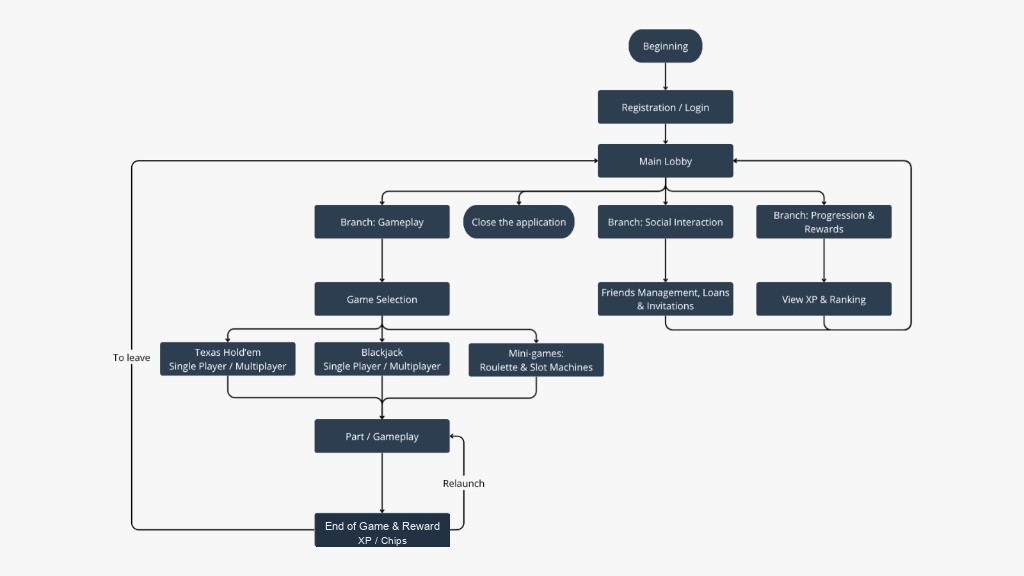
\includegraphics[width=0.95\textwidth,keepaspectratio]{user-workflow-diagram.png}
\caption{Mini user workflow: authentication, lobby entry, gameplay selection, social interaction, progression/reward consultation, exit and replay loops.}
\label{fig:user-workflow-diagram}
\end{figure}

\subsection{Representative UI captures}
\label{subsec:ui-screenshot-placeholders}

Figure~\ref{fig:ui-admin-console} shows the deployed \textbf{admin web console} (\path{/admin/console}). Figure~\ref{fig:ui-poker-table} shows an active \textbf{Texas Hold'em} table with \textbf{multiple bot opponents} on a post-flop street. Figure~\ref{fig:ui-lobby} shows the \textbf{main lobby hub}. Figure~\ref{fig:ui-tournament} shows a \textbf{tournament} registration/waiting view (scheduled event, blinds/stack, hidden winner-side bets). Figure~\ref{fig:ui-blackjack} shows the \textbf{solo blackjack} table during the betting phase. Figure~\ref{fig:ui-leaderboard} shows \textbf{public leaderboards} with mode tabs (general XP, poker, casino), rank table and the viewer's rank banner. Figure~\ref{fig:ui-profile-page} summarizes the \textbf{player profile}: identity, progression (XP, level, streak), virtual chip balance, badge catalogue and headline statistics. Figure~\ref{fig:ui-profile-avatars} shows \textbf{profile photo configuration}: upload constraints and the catalogue of \textbf{24} selectable preset avatars (plus custom image import). The captures below come from a demo-ready build with non-sensitive test data and illustrate user-visible outcomes rather than internal implementation detail.

\begin{figure}[htbp]
\centering
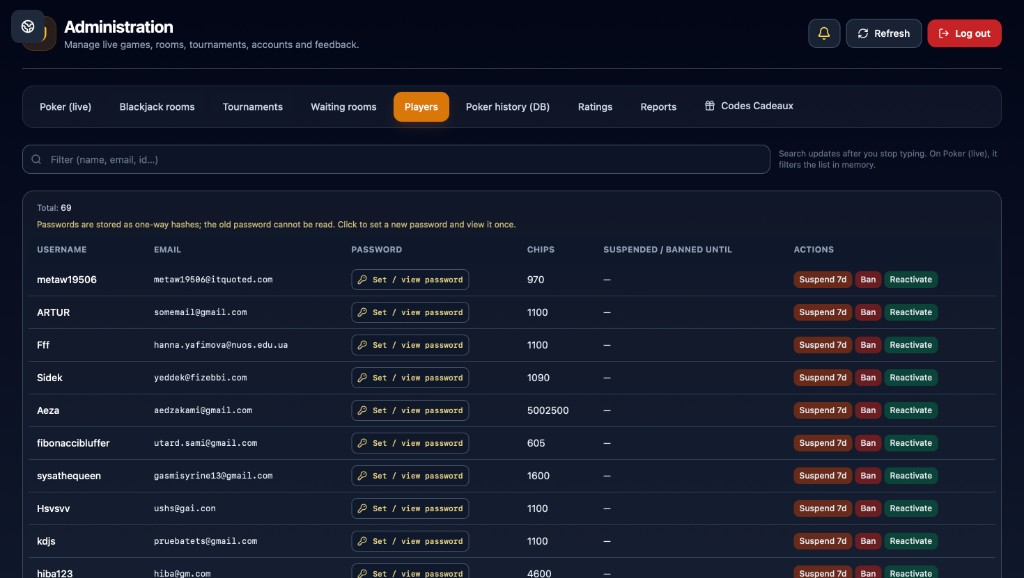
\includegraphics[width=0.95\textwidth,keepaspectratio]{screenshot-admin-console.png}
\caption{Administration dashboard (\texttt{/admin/console}): \textit{Players} tab with search, aggregate user count, reminder that passwords are stored as one-way hashes, chip balances, and moderation actions (suspend, ban, reactivate). Other tabs expose live poker, blackjack rooms, tournaments, waiting rooms, poker history (DB), ratings, reports and gift codes.}
\label{fig:ui-admin-console}
\end{figure}

\begin{figure}[htbp]
\centering
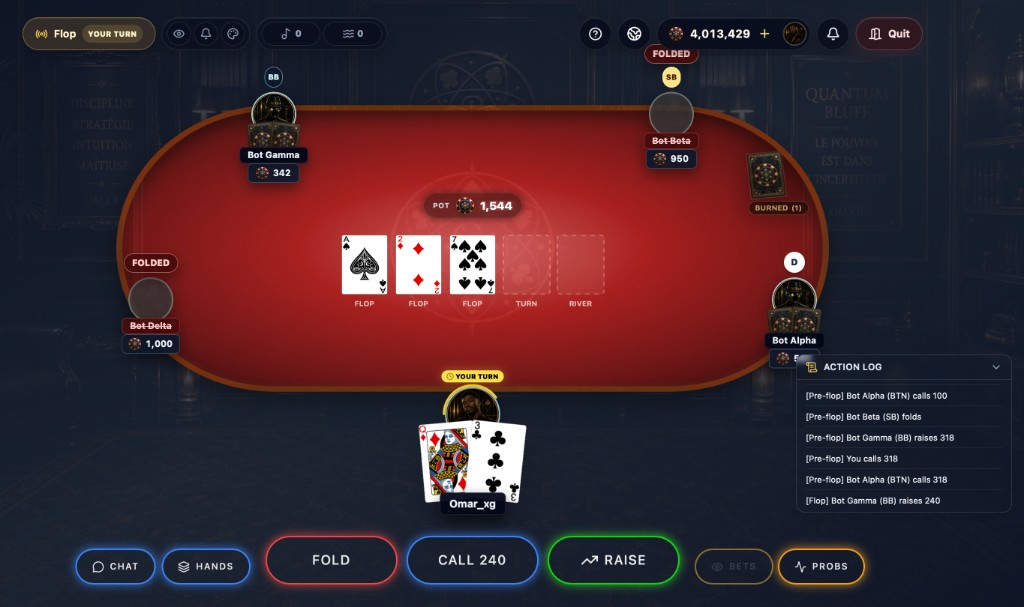
\includegraphics[width=0.95\textwidth,keepaspectratio]{screenshot-poker-table.png}
\caption{Texas Hold'em table (multi-seat vs.\ bots): \textit{Flop} street with exposed board cards, turn/river placeholders, burn-pile indicator, central pot and dealer/SB/BB badges; folded seats greyed out; hero turn with stake-aware actions (\textit{Fold} / \textit{Call} / \textit{Raise}), action log, shell chip balance and \textit{Probs} HUD entry.}
\label{fig:ui-poker-table}
\end{figure}

\begin{figure}[htbp]
\centering
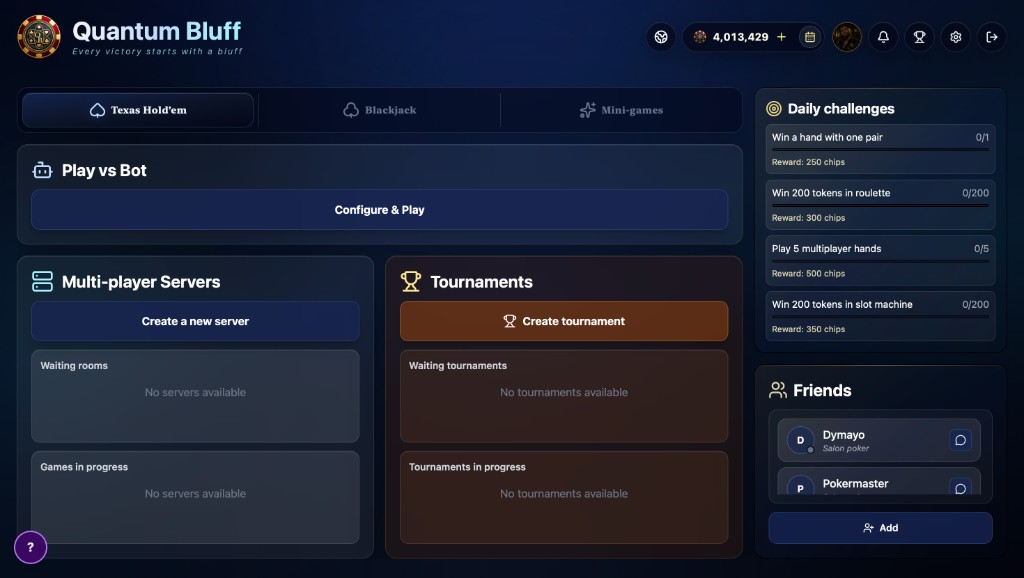
\includegraphics[width=0.95\textwidth,keepaspectratio]{screenshot-lobby.png}
\caption{Main lobby (\textit{Quantum Bluff} shell): mode tabs (Texas Hold'em, Blackjack, Mini-games), \textit{Play vs Bot}, multiplayer server lists (waiting rooms / games in progress), tournament lists with creation entry points, daily challenges with chip rewards, friends panel and global shell controls (balance, profile, settings).}
\label{fig:ui-lobby}
\end{figure}

\begin{figure}[htbp]
\centering
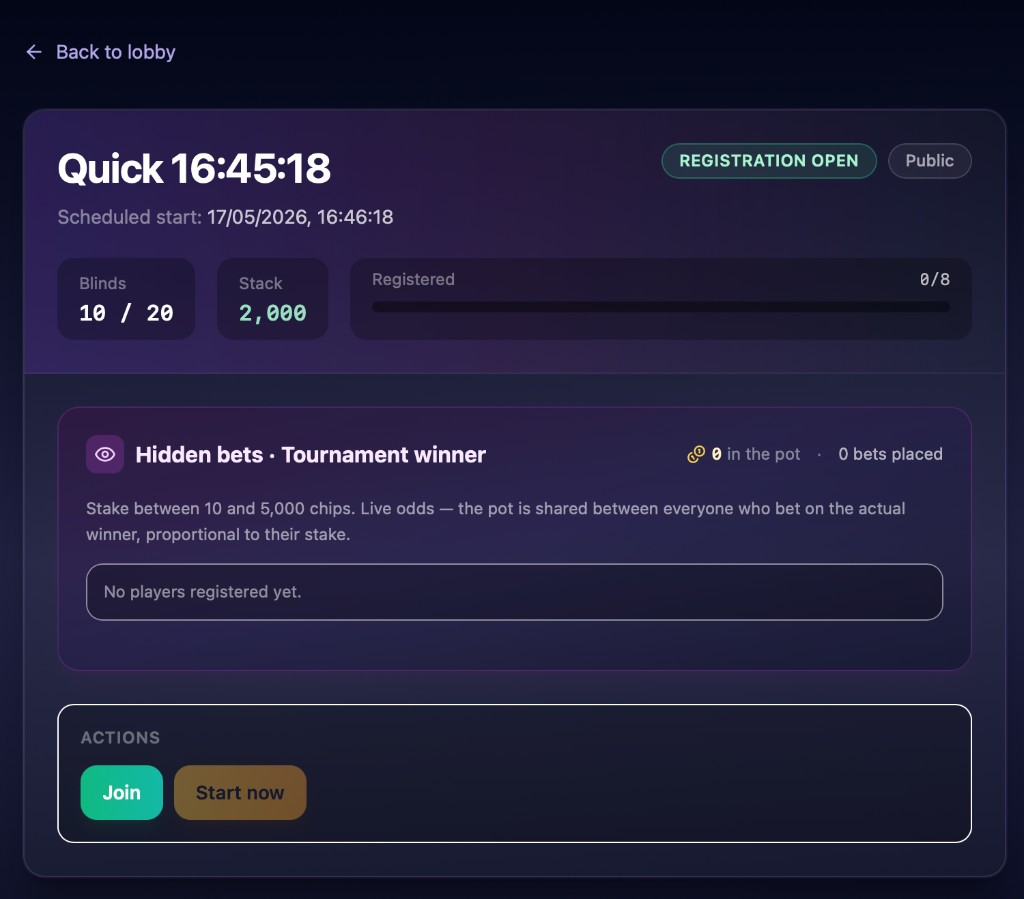
\includegraphics[width=0.95\textwidth,keepaspectratio]{screenshot-tournament.png}
\caption{Tournament lobby (waiting/registration): event title and scheduled start, status badges (\textit{Registration open}, visibility), blinds and starting stack, registration progress (e.g.\ seats filled), \textit{Hidden bets} panel for winner-side staking with pot summary, and primary actions (\textit{Join}, host-oriented \textit{Start now}).}
\label{fig:ui-tournament}
\end{figure}

\begin{figure}[htbp]
\centering
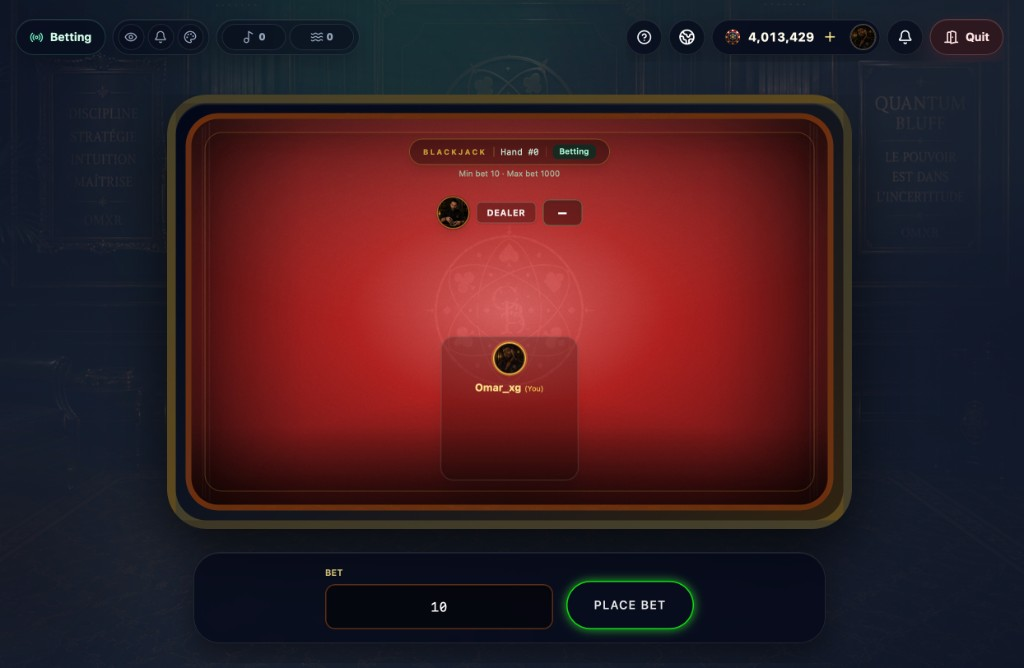
\includegraphics[width=0.95\textwidth,keepaspectratio]{screenshot-blackjack.png}
\caption{Solo blackjack table (\textit{Betting} phase before deal): status strip (hand counter, phase), published min/max stakes, dealer and player seating chrome, bet amount entry and \textit{Place bet} action, with global shell controls (chip balance, quit, audio/help shortcuts).}
\label{fig:ui-blackjack}
\end{figure}

\begin{figure}[htbp]
\centering
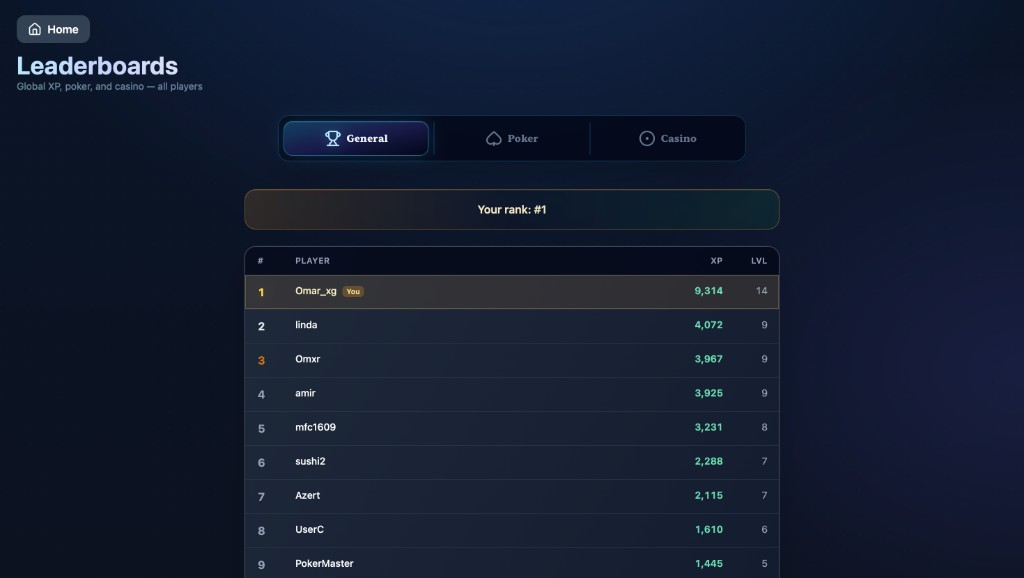
\includegraphics[width=0.95\textwidth,keepaspectratio]{screenshot-leaderboard.png}
\caption{Leaderboards (\texttt{/leaderboard}): segmented views for general XP, poker-specific and casino-specific rankings; table columns for rank, player handle, experience points and level; banner showing the signed-in player's rank; row highlight for the current user.}
\label{fig:ui-leaderboard}
\end{figure}

\begin{figure}[htbp]
\centering
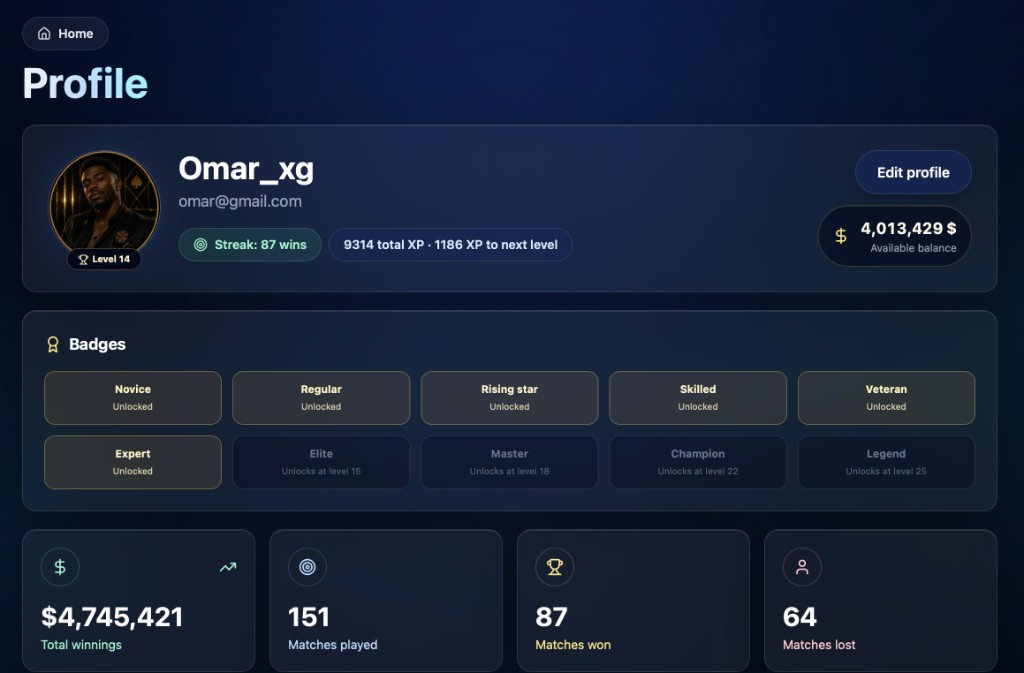
\includegraphics[width=0.95\textwidth,keepaspectratio]{screenshot-profile-page.png}
\caption{Profile hub (\texttt{/profile}): summary card with avatar, level badge, handle and email, streak/XP ribbon, available chip balance and \textit{Edit profile} entry; \textit{Badges} grid contrasting unlocked tiers with level-gated tiers; aggregate statistics (winnings, matches played/won/lost).}
\label{fig:ui-profile-page}
\end{figure}

\begin{figure}[htbp]
\centering
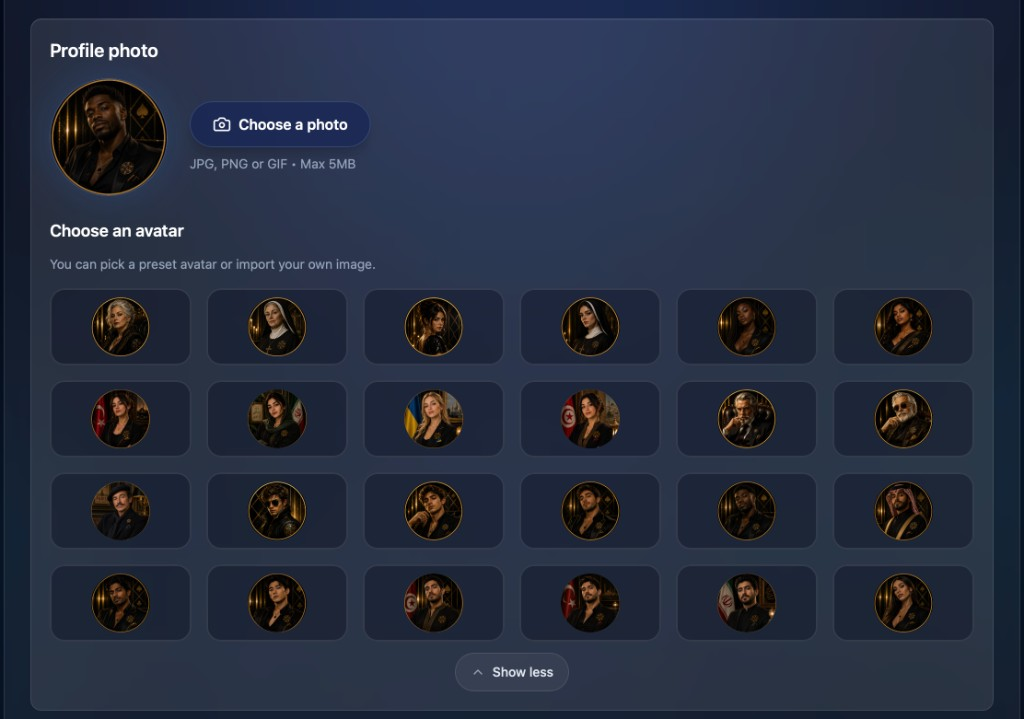
\includegraphics[width=0.95\textwidth,keepaspectratio]{screenshot-profile-avatars.png}
\caption{Profile editor --- avatar selection: circular preview, \textit{Choose a photo} upload entry with stated constraints (JPG/PNG/GIF, max 5\,MB), and a grid of \textbf{24} built-in preset portraits; players may pick a preset or supply their own image.}
\label{fig:ui-profile-avatars}
\end{figure}

\subsection{Admin and support flow}

\begin{itemize}
\item \textbf{Admin console}: authorized admins access \path{/admin/console} to inspect reports, gift codes, monitoring-oriented information and moderation data.
\item \textbf{Feedback and reports}: players can submit feedback or reports; these are persisted for later review instead of remaining client-only messages.
\item \textbf{Safety note}: the product uses simulated payments and virtual chips. It is not connected to real bank cards, real bank accounts or real-money gambling providers.
\end{itemize}

\section{Test coverage metrics and definitions}
\label{app:coverage}

\subsection{Jest ratios}

Let $L$ be the set of executable lines inside \texttt{collectCoverageFrom} in \path{jest.config.cjs}. For each metric $M\in\{\mathrm{lines},\mathrm{statements},\mathrm{functions},\mathrm{branches}\}$,
\[
\mathrm{cov}_M = \frac{\text{\# elements of }M\text{ hit during tests}}{\text{\# elements of }M\text{ instrumented}}.
\]
CI enforces $\mathrm{cov}_{\mathrm{lines}},\mathrm{cov}_{\mathrm{statements}},\mathrm{cov}_{\mathrm{functions}}\ge 0.80$ and $\mathrm{cov}_{\mathrm{branches}}\ge 0.65$. A May~2026 local run on that scope reported:
\begin{align*}
\mathrm{cov}_{\mathrm{lines}} &= 86.56\%, &
\mathrm{cov}_{\mathrm{statements}} &= 83.69\%,\\
\mathrm{cov}_{\mathrm{functions}} &= 88.75\%, &
\mathrm{cov}_{\mathrm{branches}} &= 67.90\%.
\end{align*}
Heavy files such as \path{botAI.ts} and large controllers are deliberately excluded from the denominator so the metric tracks testable business modules (see comments in the Jest config).

\subsection{Vitest ratios (client)}

Vitest with Istanbul uses the same hit/total idea over the frontend TypeScript source files minus tests. Because most screens depend on sockets and browser APIs, the \textbf{global} line coverage stays low unless many components receive dedicated tests; quality is also asserted through Playwright flows and manual regression lists.

\subsection{Relation to tournaments}

Bracket helpers (\path{tableSizes.ts}, \path{TournamentBracketBuilder.ts}) sit inside the Jest coverage glob; their golden tests contribute directly to the aggregate in Table~\ref{tab:coverage}. See Appendix~\ref{app:tournament} for the mathematics they implement.

\subsection{Further reading}

\path{test_coverage.md}, \path{TESTING_GUIDE.md}, \path{RAPPORT_TESTS.md}.

\section{Real-time and security details}
\label{app:rt-security-solutions}

\subsection{Real-time communication details}

Real-time communication is implemented with Socket.IO on the \texttt{/socket.io} path. The design follows an authoritative server model: the browser can request an action, but the server decides whether the user is authenticated, whether the action is legal, how chips move, and which sanitized state each participant may receive. This is essential for poker because private cards, turn order, pot resolution and hidden side bets must never be trusted to the client.

The socket handshake uses the same identity model as the REST API. A player token is sent through \texttt{handshake.auth.token} or an \texttt{Authorization: Bearer ...} header, then validated by \path{socketAuth.middleware.ts} and gateway-level checks in \path{game.gateway.ts}. The server verifies token revocation, JWT issuer/audience/type, role separation, user existence and suspension status before attaching the authenticated user id to the socket.

Socket.IO rooms organize delivery. Each user joins \texttt{user:\{userId\}} for targeted events such as invitations, tournament assignments, blocked-user warnings and social notifications. Poker and blackjack tables use table rooms; tournaments use rooms such as \texttt{tournament:\{id\}}. This prevents unrelated users from receiving game or social events that do not concern them.

Game synchronization combines incremental events with full snapshots. Poker runtime controllers are tracked through \path{activeGames.ts}; serializable poker snapshots are stored through \path{pokerStateStore.ts} and produced by \path{pokerStateSync.service.ts}. Blackjack recovery and snapshot logic lives under \path{recovery} and \path{services}. On join or reconnect, the client receives a full sanitized snapshot so a refresh or temporary disconnection does not leave the UI in a stale state.

Sanitization protects confidentiality. A seated poker player can receive their own private cards, while other players and spectators receive only public table information. Redis support through \path{socketIoRedis.ts} allows Socket.IO events to propagate across multiple server instances.

\subsection{Authentication and anti-cheat details}

Authentication is based on short-lived JWT access tokens generated by \path{jwt.service.ts}. Tokens must use the expected issuer, audience and \texttt{type: access}. HTTP routes accept only the standard \texttt{Authorization: Bearer ...} form, and protected routes use \path{auth.middleware.ts} to reject revoked tokens, invalid tokens, admin-role tokens on player routes, missing users and suspended accounts.

Passwords are hashed with bcrypt in \path{auth.routes.ts}. Registration, reset and profile password changes use Zod validation from \path{auth.validation.ts}, including complexity requirements. Optional TOTP two-factor authentication is implemented in \path{twofa.routes.ts}; setup secrets are stored temporarily in Redis, and disabling 2FA requires both the password and a valid one-time code. Logout and token revocation use \path{tokenBlacklist.ts}, which stores hashed token entries with expiration.

The same identity policy applies to WebSockets. \path{socketAuth.middleware.ts} rejects revoked, invalid, admin, missing-user and suspended-user tokens before a socket can interact with game rooms. In \path{game.gateway.ts}, sensitive events compare \texttt{socket.userId} with any submitted player id; mismatches are refused and logged as suspicious.

Anti-cheat is layered. \path{antiCheat.middleware.ts} blocks active bans, records the last observed IP address and delegates suspicious-pattern detection to \path{antiCheat.service.ts}. The service can raise alerts for multi-account patterns and unrealistically fast reactions. At game level, \path{antiCheat.ts} tracks action bursts and helps refuse excessive gameplay actions.

Operational safeguards complete the baseline: Helmet and CORS allowlists in \path{index.ts}, segmented rate limits for sensitive endpoints, idempotency middleware for sensitive mutations in \path{idempotency.middleware.ts}, separated admin routes, blocked-user filtering, blocked-room warnings and persisted player reports for moderation review.

\section{External references and compendium}
\label{app:sources}

\begin{itemize}
\item Initial formal requirements PDF: \path{Cahier_de_charge_6A_PI.pdf} (not embedded here).
\item Auto-generated wide-coverage technical compendium: \path{RAPPORT_TECHNIQUE_COMPLET.md} (use as index; verify claims against code).
\item Security dossiers: \path{SECURITE_A_TO_Z.md}, \path{security}.
\item HTTP and socket maps: \path{01_http_api_map.md}, \path{02_socket_events_map.md}.
\item Combination analysis report: \path{QUANTUM_COMBI.adoc}.
\item Slot RTP and outcome algebra (AsciiDoc): \path{SLOT_MACHINE.adoc}.
\item Roulette payouts and expectation: \path{ROULETTE.adoc}.
\end{itemize}

\clearpage
\begin{thebibliography}{99}

\bibitem{react19}
Meta. \textit{React documentation} (React 19). \url{https://react.dev/} (accessed May 2026).

\bibitem{typescript}
Microsoft. \textit{TypeScript handbook.} \url{https://www.typescriptlang.org/docs/} (accessed May 2026).

\bibitem{vite}
Vite contributors. \textit{Vite guide.} \url{https://vite.dev/guide/} (accessed May 2026).

\bibitem{nodejs}
OpenJS Foundation. \textit{Node.js runtime documentation.} \url{https://nodejs.org/docs/latest/api/} (accessed May 2026).

\bibitem{express}
OpenJS Foundation. \textit{Express web framework.} \url{https://expressjs.com/} (accessed May 2026).

\bibitem{socketio}
Socket.IO project. \textit{Socket.IO server and client (v4).} \url{https://socket.io/docs/v4/} (accessed May 2026).

\bibitem{prisma}
Prisma Data Inc. \textit{Prisma ORM documentation.} \url{https://www.prisma.io/docs} (accessed May 2026).

\bibitem{postgresql}
PostgreSQL Global Development Group. \textit{PostgreSQL documentation.} \url{https://www.postgresql.org/docs/} (accessed May 2026).

\bibitem{redis}
Redis Ltd. \textit{Redis documentation.} \url{https://redis.io/docs/} (accessed May 2026).

\bibitem{redux}
Redux team. \textit{Redux Toolkit and RTK Query.} \url{https://redux-toolkit.js.org/} (accessed May 2026).

\bibitem{i18next}
i18next authors. \textit{i18next documentation.} \url{https://www.i18next.com/} (accessed May 2026).

\bibitem{zod}
Zod maintainers. \textit{Zod schema validation.} \url{https://zod.dev/} (accessed May 2026).

\bibitem{jest}
OpenJS Foundation. \textit{Jest testing framework.} \url{https://jestjs.io/} (accessed May 2026).

\bibitem{vitest}
Vitest contributors. \textit{Vitest.} \url{https://vitest.dev/} (accessed May 2026).

\bibitem{playwright}
Microsoft. \textit{Playwright end-to-end testing.} \url{https://playwright.dev/} (accessed May 2026).

\bibitem{tailwind}
Tailwind Labs. \textit{Tailwind CSS documentation.} \url{https://tailwindcss.com/docs} (accessed May 2026).

\bibitem{scrumguide}
Schwaber, K., Sutherland, J. \textit{The Scrum Guide} (2020). \url{https://scrumguides.org/scrum-guide.html} (accessed May 2026).

\bibitem{gitlabci}
GitLab Inc. \textit{GitLab CI/CD documentation.} \url{https://docs.gitlab.com/ee/ci/} (accessed May 2026).

\bibitem{unistra}
Université de Strasbourg. \textit{Faculté des mathématiques et informatique.} \url{https://mathinfo.unistra.fr/} (accessed May 2026).

\end{thebibliography}

\end{document}
